\documentclass{eic-bcc-tcc}

\title{Hedge-fund-lab: Laboratório Quantitativo de Backtesting baseado em Sistemas Multiagentes}
\titleen{Hedge-fund-lab: Quantitative Backtesting Laboratory based on Multi-agent Systems}

\addstudent[Lucas Pereira da Silva]{Lucas Pereira da Silva}
\addstudent[Matheus Pereira de Carvalho]{Matheus Pereira de Carvalho}

\newcommand{\warn}[1]{{\color{red} {#1}}}
\newcommand{\verify}[1]{{\color{blue} {#1}}}
\newcommand{\remarks}[2]{{\color{red} #1\ (\textit{#2})}}

\advisor[m]{Eduardo Soares Ogasawara, D.Sc.}
\addboardmember{Membro Interno}{}
\addboardmember{Membro Externo}{}

\date{2026}

\newacronym{tcc}{TCC}{Trabalho de Conclusão de Curso}
\newacronym{rsi}{RSI}{Relative Strength Index}
\newacronym{sma}{SMA}{Simple Moving Average}
\newacronym{macd}{MACD}{Moving Average Convergence Divergence}
\newacronym{dp}{DP}{Decisão de Projeto}
\newacronym{jcp}{JCP}{Juros sobre Capital Próprio}
\newacronym{ohlcv}{OHLCV}{Open, High, Low, Close, Volume}
\newacronym{mar}{MAR}{Minimum Acceptable Return}
\newacronym{http}{HTTP}{Hypertext Transfer Protocol}
\newacronym{json}{JSON}{JavaScript Object Notation}
\newacronym{sql}{SQL}{Structured Query Language}
\newacronym{csv}{CSV}{Comma-Separated Values}
\newacronym{sha}{SHA}{Secure Hash Algorithm}

\usepackage{tikz}
\usepackage{placeins}
\usetikzlibrary{arrows.meta, positioning}
\usepackage{pgfplots} % figuras do replay (figures/replay-*.tex)
\pgfplotsset{compat=1.18}

% Nomes longos em \texttt{} (caminhos de código) não hifenizam; folga extra evita
% que estourem a margem.
\setlength{\emergencystretch}{3em}
\usepackage[htt]{hyphenat} % hifeniza \texttt e permite quebra após \_
% ponytail: a classe usa \MakeUppercase sem argumento nos títulos do tocloft, o que
% quebra ("Missing \endcsname") com o LaTeX/tocloft do MiKTeX de 2026. Aqui os nomes
% já vêm em maiúsculas e a fonte não converte. Se a classe for corrigida, remova.
\renewcommand{\cftloftitlefont}{\hfill\large\bfseries}
\renewcommand{\cftlottitlefont}{\hfill\bfseries\large}
\renewcommand{\cfttoctitlefont}{\hspace{0.4\textwidth}\large\bfseries}
\addto\captionsbrazil{%
  \renewcommand{\listfigurename}{LISTA DE FIGURAS}%
  \renewcommand{\listtablename}{LISTA DE TABELAS}%
  \renewcommand{\contentsname}{SUMÁRIO}}

\begin{document}

\maketitle

\makeapproval

\begin{resumo}
A avaliação de estratégias quantitativas em mercados não estacionários é sujeita a custos, dependência de regime e superajuste. Este trabalho apresenta o Hedge-fund-lab, laboratório quantitativo de \textit{backtesting} baseado em sistemas multiagentes, e o emprega para verificar se uma carteira decidida por agentes baseados em \textit{Large Language Models} (LLMs) apresenta desempenho ajustado ao risco superior ao de carteiras de referência clássicas. O laboratório integra dados oficiais da B3 (COTAHIST), um livro contábil de eventos auditável e comitês de analistas técnicos, analistas de risco e um gestor de carteira, cuja proposta é submetida a um compilador determinístico de regras. O estudo empírico é um replay retrospectivo de 153 pregões, de abril a novembro de 2026, com cinco ações e R\$ 100 mil por carteira, no qual a carteira multiagente é comparada a cinco referências determinísticas (Buy \& Hold, SMA 50/200, Bollinger 20/2, Equal Weight e Mínima Variância) em três versões: a v1, pré-especificada, e as v2 e v3, iterações exploratórias desenhadas após a observação do mesmo período. As hipóteses são decididas pelo Sharpe líquido com \textit{bootstrap} estacionário pareado (Bootstrap A). A v1 terminou em $-17{,}82\%$, abaixo das cinco referências, e nenhum de seus contrastes rejeitou a hipótese nula; a SMA 50/200 tampouco superou a Equal Weight. A v3 terminou em $+0{,}07\%$, acima de quatro referências e abaixo da Bollinger 20/2 ($+4{,}89\%$), resultado otimista por construção. Conclui-se que não há evidência de superioridade dos agentes e que, nesta trajetória, a especialização do comitê e a governança determinística alteraram de forma mensurável o comportamento da carteira. A avaliação livre de contaminação do modelo depende do acompanhamento prospectivo, já em curso.
\palavraschave{Análise Quantitativa. Sistemas Multiagentes. Large Language Models. Backtesting. Mercado Acionário Brasileiro.}
\end{resumo}

\begin{abstract}
The evaluation of quantitative strategies in non-stationary markets is subject to costs, regime dependence, and overfitting. This work presents the Hedge-fund-lab, a quantitative backtesting laboratory based on multi-agent systems, and uses it to test whether a portfolio managed by agents based on Large Language Models (LLMs) achieves higher risk-adjusted performance than classical benchmark portfolios. The laboratory integrates official B3 trading records (COTAHIST), an auditable event ledger, and committees of technical analysts, risk analysts, and a portfolio manager whose proposal is submitted to a deterministic rule compiler. The empirical study is a retrospective replay of 153 trading sessions, from April to November 2026, with five stocks and BRL 100,000 per portfolio, in which the multi-agent portfolio is compared with five deterministic benchmarks (Buy \& Hold, SMA 50/200, Bollinger 20/2, Equal Weight, and Minimum Variance) in three versions: v1, pre-specified, and v2 and v3, exploratory iterations designed after observing the same period. The hypotheses are decided on the net Sharpe ratio with a paired stationary bootstrap (Bootstrap A). Version v1 ended at $-17.82\%$, below all five benchmarks, and none of its contrasts rejected the null hypothesis; SMA 50/200 did not outperform Equal Weight either. Version v3 ended at $+0.07\%$, above four benchmarks and below Bollinger 20/2 ($+4.89\%$), a result optimistic by construction. The study concludes that there is no evidence of agent superiority and that, along this trajectory, committee specialization and deterministic governance measurably changed the portfolio's behavior. An evaluation free from model contamination depends on the prospective daily tracking already under way.
\keywords{Quantitative Analysis. Multi-Agent Systems. Large Language Models. Backtesting. Brazilian Stock Market.}
\end{abstract}

\listoffigurespage

\begingroup
  \let\cleardoublepage\clearpage
  \listoftablespage
  \listofacronymspage
\endgroup

\tableofcontentspage

\mainmatter

\chapter{Introdução}
\glsaddall[types={\acronymtype}]
\label{cha:introducao}

O mercado financeiro contemporâneo impõe desafios relevantes à construção e à avaliação de estratégias quantitativas, sobretudo em cenários marcados por alta volatilidade, não estacionariedade e grande volume de dados. Nesse contexto, abordagens clássicas de análise técnica continuam úteis como referência metodológica, mas frequentemente apresentam limitações quando aplicadas de forma isolada, seja pela sensibilidade a regimes de mercado distintos, seja pelo risco de superajuste (\textit{overfitting}) em processos de \textit{backtesting}. Essa constatação justifica a proposição de um ambiente experimental capaz de organizar dados, regras de decisão e critérios de avaliação de maneira rigorosa, antes da busca por desempenho superior imediato.

Diante desse cenário, o problema central desta pesquisa consiste em como conceber uma arquitetura de laboratório de \textit{backtesting} que integre engenharia de dados e deliberação multiagente baseada em \textit{Large Language Models} (LLMs), permitindo uma comparação robusta com \textit{benchmarks} clássicos. A pergunta de pesquisa que orienta o trabalho pode ser formulada da seguinte maneira: como projetar um ambiente experimental que permita avaliar, de forma comparável e metodologicamente controlada, se uma arquitetura multiagente baseada em LLMs produz decisões de investimento mais robustas do que abordagens tradicionais quando submetida a critérios explícitos de risco, custo e consistência operacional?

Com esse propósito, este trabalho tem como objetivo geral desenvolver o Hedge-fund-lab, um laboratório quantitativo para \textit{backtesting} de estratégias de investimento baseado em sistemas multiagentes. Como contribuição principal, propõe-se a avaliação comparativa entre metodologias clássicas de alocação e uma arquitetura de inteligência artificial baseada em deliberação multiagente. Para viabilizar essa análise empírica, o trabalho desenvolve um artefato metodológico que integra um pipeline de dados baseado nos registros oficiais de negociação da B3 (COTAHIST), persistidos em banco relacional (SQLite/SQLAlchemy), a um sistema multiagente com papéis especializados em análise técnica, gestão de risco e gestão de portfólio --- implementado como grafo LangGraph para um único ativo e como carteira multiativos com capital compartilhado ---, executado sobre mecanismos próprios de simulação e contabilidade, permitindo uma mensuração rigorosa de desempenho frente aos \textit{benchmarks} tradicionais.

O protocolo confirmatório planejado na etapa anterior do trabalho, com fases de calibração e um Teste Final isolado sobre um único ativo, não chegou a ser executado (Seção~\ref{sec:met-protocolo}). O estudo empírico pelo qual as hipóteses são respondidas é o Replay Contínuo Abril--Novembro de 2026: uma reconstrução retrospectiva de 153 pregões da B3, de 06/04/2026 a 12/11/2026, com cinco ações (BBAS3, ITUB4, PETR4, VALE3 e WEGE3) e R\$ 100.000,00 por carteira, na qual a carteira Multiagentes e cinco carteiras de referência determinísticas --- Buy \& Hold, SMA 50/200, Bollinger 20/2, Equal Weight 63d e Mínima Variância 252/63 --- percorrem a mesma trajetória de mercado, com os mesmos preços, custos e cesta inicial. A carteira Multiagentes foi executada em três versões sucessivas: a v1, pré-especificada, cujas regras foram fixadas antes de qualquer observação de seu desempenho no replay; e as v2 e v3, iterações exploratórias desenhadas após a auditoria das versões anteriores sobre o mesmo período. Como o replay foi produzido depois do fim do período e o modelo pode conhecê-lo por seu treinamento, a avaliação livre dessa contaminação é o acompanhamento diário prospectivo da carteira, iniciado em 14/10/2026, que constitui a continuação do estudo.

A comparação entre as três versões responde a uma pergunta secundária, de natureza arquitetural e exploratória: mantidos o modelo de linguagem, a quantidade de agentes, os dados e as regras de execução, quanto do comportamento da carteira multiagente depende da especialização dos analistas e da governança determinística aplicada sobre a proposta do gestor?

São objetivos específicos do trabalho:

\begin{enumerate}
    \item Construir um pipeline de dados reproduzível, a partir da fonte oficial de preços e negociações da B3 (COTAHIST), com correção de proventos e calendário de negociação próprio;
    \item Implementar um motor de \textit{backtesting} e um livro contábil de eventos auditável que incorporem custos de transação, proventos e as métricas de risco definidas no protocolo experimental;
    \item Desenvolver um sistema multiagente baseado em LLMs, com papéis especializados e processo de consenso, nas versões de ativo único (coordenada por LangGraph) e multiativos (com gestor global da carteira e compilador determinístico da proposta do modelo);
    \item Estabelecer um desenho experimental pareado e causal, com métrica primária e regra de decisão estatística definidas, que permita comparar o sistema multiagente aos \textit{benchmarks} clássicos sem vazamento de informação futura nos dados entregues aos agentes;
    \item Executar o Replay Contínuo Abril--Novembro de 2026 e analisar a evolução da arquitetura entre as três versões da carteira Multiagentes, com decisões, operações e patrimônio rastreáveis;
    \item Operar a carteira multiativos em acompanhamento diário prospectivo, como base para a avaliação livre de contaminação.
\end{enumerate}

A partir do referencial teórico, formulam-se as seguintes hipóteses de pesquisa, preservadas integralmente da etapa anterior do trabalho:

\begin{itemize}
    \item \textbf{H1:} Será avaliado se estratégias baseadas em momentum e \textit{trend following} apresentam desempenho superior ao \textit{equal weight} em termos de Sharpe Ratio líquido.
    \item \textbf{H2:} Será avaliado se o sistema multiagente baseado em LLMs apresenta desempenho superior ajustado ao risco em relação aos \textit{benchmarks} considerados, tomando como critério principal o Sharpe Ratio líquido e, como critérios complementares, Sortino Ratio, \textit{Maximum Drawdown} e \textit{turnover}.
    \item \textbf{H0:} Não há diferença estatisticamente significativa entre as abordagens.
\end{itemize}

No replay, H1 é operacionalizada pelo contraste de Sharpe entre a SMA 50/200 e a Equal Weight 63d, e H2 pelos contrastes da versão v1 com cada uma das cinco referências; H0 é decidida em cada família por \textit{bootstrap} estacionário pareado. Os contrastes das versões v2 e v3 são apenas descritivos (Seção~\ref{sec:met-hipoteses}).

A contribuição deste trabalho é menos a antecipação de um resultado de desempenho superior e mais o estabelecimento de uma base técnica e metodológica coerente para a avaliação de agentes baseados em LLMs: um laboratório quantitativo reproduzível, auditável e extensível, em que dados, estratégias e critérios de avaliação são rastreados de forma explícita. Sobre essa base, o trabalho contribui com uma comparação pareada entre gerações de uma mesma arquitetura multiagente, com modelo, topologia de agentes, dados, execução e carteiras de referência constantes; com a medida da homogeneidade de comitês formados por instâncias de um mesmo modelo e de sua redução por especialização dos papéis; com um padrão de governança determinística em que cada intervenção sobre a proposta do modelo é registrada; e com o registro de resultados negativos, conduzido de modo a evitar o viés de superajuste que caracteriza boa parte da literatura aplicada.

A presente monografia está organizada em sete capítulos. Além desta introdução, o Capítulo~\ref{cha:fundamentacao} apresenta a fundamentação teórica, abordando as hipóteses de eficiência de mercado, os \textit{benchmarks} simples, as estratégias de análise técnica, a teoria moderna de portfólio, os sistemas multiagentes baseados em modelos de linguagem e as métricas de desempenho e risco. O Capítulo~\ref{cha:relacionados} revisa os trabalhos relacionados, com atenção à avaliação de LLMs em finanças e à contaminação temporal, e situa o Hedge-fund-lab frente às abordagens existentes. O Capítulo~\ref{cha:arquitetura} descreve a arquitetura e a implementação da solução: o pipeline de dados, a persistência e o livro contábil, o motor de \textit{backtesting}, os dois caminhos multiagentes, o mecanismo do replay, a evolução da arquitetura entre as versões e a operação diária. O Capítulo~\ref{cha:metodologia} detalha o desenho do replay, a operacionalização das hipóteses, as métricas, a inferência estatística, o protocolo confirmatório planejado e as ameaças à validade. O Capítulo~\ref{cha:resultados} apresenta e discute os resultados do replay e a observação preliminar do acompanhamento diário, e o Capítulo~\ref{cha:conclusao} encerra com as respostas às perguntas de pesquisa, as limitações e os trabalhos futuros.

\chapter{Fundamentação Teórica}
\label{cha:fundamentacao}

\section{HIPÓTESE DE EFICIÊNCIA DE MERCADO}

A Hipótese de Eficiência de Mercado (\textit{Efficient Market Hypothesis} -- EMH), formalizada por \citep{Fama1970}, postula que os preços dos ativos financeiros refletem integralmente todas as informações disponíveis. Consequentemente, não seria possível obter retornos anormais de forma consistente utilizando exclusivamente informações públicas ou históricas, uma vez que tais dados já estariam incorporados aos preços.

No mesmo trabalho, Fama classifica a eficiência de mercado em três níveis:

\begin{itemize}
\item Forma fraca: os preços refletem apenas informações históricas de preço e volume;
\item Forma semi-forte: os preços incorporam todas as informações públicas disponíveis;
\item Forma forte: os preços refletem todas as informações, inclusive as privadas.
\end{itemize}

A relevância dessa hipótese para o presente trabalho reside no debate sobre a previsibilidade dos retornos financeiros. Em um mercado perfeitamente eficiente, estratégias quantitativas baseadas em padrões históricos não seriam capazes de gerar retornos superiores de forma consistente. Contudo, evidências empíricas apontam para a existência de anomalias de mercado, como os efeitos momentum e \textit{value premium} \citep{FamaFrench1992, JegadeeshTitman1993}.

\subsection{Críticas Comportamentais e a Hipótese de Mercados Adaptativos}

Apesar de sua relevância teórica, a EMH recebeu críticas substanciais da economia comportamental. Estudos de \citep{Shiller2000} e \citep{Thaler1993} demonstram que vieses cognitivos, como excesso de confiança, aversão à perda e comportamento de manada, podem levar a desvios persistentes entre preços de mercado e valores fundamentais.

Buscando reconciliar a racionalidade da EMH com as evidências comportamentais, \citet{Lo2004} propôs a Hipótese de Mercados Adaptativos (\textit{Adaptive Markets Hypothesis} -- AMH). Neste modelo, a eficiência de mercado não é um estado fixo, mas um processo dinâmico que evolui ao longo do tempo conforme os agentes aprendem e se adaptam às mudanças no ambiente econômico.

Essa perspectiva fornece suporte teórico para o uso de sistemas baseados em inteligência artificial e modelos de linguagem, uma vez que modelos adaptativos e multiagentes podem capturar padrões dinâmicos e interpretar contextos que estratégias estáticas ou puramente matemáticas não conseguem identificar.

\section{BENCHMARKS SIMPLES: BUY AND HOLD E EQUAL WEIGHT}

Estratégias quantitativas tradicionais e \textit{benchmarks} cumprem o papel de base comparativa essencial na avaliação de sistemas de decisão, pois oferecem referências de implementação simples e menos dependentes de estimações sofisticadas, o que facilita o contraste com abordagens mais complexas de alocação e seleção de sinais \citep{Markowitz1952, Clarke2006, LopezDePrado2018}.

\subsection{Buy and Hold}
\textit{Buy and Hold} é uma estratégia passiva em que o investidor compra um ativo ou uma carteira de ativos e permanece posicionado durante todo o período de avaliação. Em estudos de \textit{backtesting}, sua utilidade metodológica reside em fornecer uma linha de base de baixa complexidade, útil para verificar se uma estratégia ativa gera valor além da simples exposição ao mercado após a consideração de risco e custos operacionais \citep{LopezDePrado2018, Bailey2017}. No contexto deste trabalho, esse \textit{benchmark} permite distinguir eventuais ganhos associados ao processo de deliberação dos agentes daqueles que decorreriam apenas do comportamento geral dos ativos analisados.

\subsection{Equal Weight}
\textit{Equal Weight}, ou carteira igualmente ponderada, consiste em distribuir o capital igualmente entre os ativos selecionados. Sua relevância decorre do fato de incorporar diversificação sem recorrer diretamente à estimação de parâmetros como retorno esperado e matriz de covariância, exigidos por modelos de otimização clássicos \citep{Markowitz1952, Clarke2006, DeMiguel2009}. Por essa razão, trata-se de um \textit{benchmark} particularmente útil para comparar abordagens sofisticadas com uma regra simples de alocação, permitindo avaliar se o aumento de complexidade metodológica se traduz, de fato, em ganhos consistentes de desempenho ajustado ao risco.

\section{ESTRATÉGIAS BASEADAS EM ANÁLISE TÉCNICA}

A análise técnica assume que padrões históricos de preços e indicadores derivados dessas séries temporais podem gerar sinais úteis para previsão de movimentos futuros do mercado. \citet{Brock1992} investigam regras técnicas simples e mostram que tais procedimentos podem ser avaliados empiricamente por meio de simulações históricas. Da mesma forma, \citet{Lo2000} tratam padrões gráficos sob uma perspectiva estatística, reforçando o uso de estratégias técnicas como \textit{benchmarks} quantitativos.

\subsection{Estratégias de Tendência (Trend Following)}

Estratégias de \textit{trend following} buscam explorar a persistência de movimentos de preço. O \textit{Moving Average Crossover} é uma estratégia técnica clássica baseada no cruzamento entre médias móveis de diferentes horizontes. \citet{Brock1992} demonstram que regras baseadas em médias móveis apresentam poder preditivo estatisticamente significativo. A média móvel simples é definida como:

\begin{equation}
MA_t = \frac{1}{n} \sum_{i=0}^{n-1} P_{t-i}
\end{equation}

Quando uma média curta cruza acima de uma média longa, interpreta-se como um sinal de tendência positiva. Essa regra traduz a ideia de acompanhamento de tendência em um critério operacional claro.

Outra medida amplamente utilizada é o momentum, definido como o retorno acumulado em uma janela temporal:

\begin{equation}
Momentum_t = \frac{P_t}{P_{t-n}} - 1
\end{equation}

\citet{JegadeeshTitman1993} mostram que estratégias baseadas em momentum produzem retornos anormais positivos. A ideia central é que ativos com desempenho positivo em uma janela recente tendem a continuar apresentando desempenho superior \citep{Moskowitz2012}.

\subsection{Estratégias de Reversão à Média (Mean Reversion)}

A hipótese de reversão à média (\textit{Mean Reversion}) pressupõe que desvios expressivos em relação a um nível considerado normal tendem a ser parcialmente revertidos ao longo do tempo. \citet{PoterbaSummers1988} investigam componentes transitórios e encontram evidências de reversão à média em horizontes de longo prazo. O sinal de negociação pode ser obtido por meio do z-score:

\begin{equation}
z_t = \frac{P_t - \mu}{\sigma}
\end{equation}

onde $\mu$ representa a média móvel e $\sigma$ o desvio padrão. A lógica consiste em comprar ativos que registraram queda recente ou reduzir a exposição a ativos que subiram acentuadamente.

Entre os indicadores mais utilizados destacam-se o Índice de Força Relativa (RSI), proposto por \citet{Wilder1978}, e as Bandas de Bollinger, introduzidas por \citet{Bollinger2001}. As Bandas de Bollinger são definidas por:

\begin{equation}
BB_{upper} = MA + k\sigma
\end{equation}

\begin{equation}
BB_{lower} = MA - k\sigma
\end{equation}

O RSI busca medir a intensidade dos movimentos recentes de alta e baixa de um ativo, identificando sobrecompra ou sobrevenda. A esses indicadores soma-se o MACD (\textit{Moving Average Convergence Divergence}), que combina a diferença entre duas médias exponenciais e sua linha de sinal para identificar mudanças de tendência. A comparação entre \textit{momentum} e \textit{mean reversion} é relevante porque essas estratégias representam hipóteses opostas sobre a dinâmica dos retornos e, em mercados sujeitos a mudanças de regime, podem atuar de forma complementar \citep{JegadeeshTitman1993, PoterbaSummers1988, Moskowitz2012}.

\section{FACTOR INVESTING E MODELOS DE PRECIFICAÇÃO DE ATIVOS}

Enquanto a análise técnica foca em padrões históricos de preços, o \textit{Factor Investing} busca explicar retornos a partir de características fundamentais das empresas. O modelo de três fatores de \citep{FamaFrench1993} é um dos mais influentes:

\begin{equation}
R_i - R_f = \beta_m (R_m - R_f) + \beta_s SMB + \beta_v HML
\end{equation}

Posteriormente, \citep{FamaFrench2015} expandiram o modelo. Estudos recentes demonstram que modelos de \textit{machine learning} podem capturar relações não lineares entre fatores de risco e retornos esperados, superando abordagens lineares tradicionais \citep{Gu2020}.

\section{TEORIA MODERNA DE PORTFÓLIO}

A Teoria Moderna de Portfólio, proposta por \citet{Markowitz1952}, estabelece uma das bases mais importantes da teoria financeira moderna. A decisão de investimento não deve considerar apenas o retorno esperado de cada ativo isoladamente, mas também o risco da carteira como um todo e as relações de covariância entre os ativos. A diversificação permite reduzir o risco total do portfólio sem necessariamente reduzir o retorno esperado. O risco de um portfólio é definido pela variância:

\begin{equation}
\sigma_p^2 = w^T \Sigma w
\end{equation}

Essa abordagem oferece um \textit{benchmark} clássico de alocação, útil como referência para comparação com estratégias mais sofisticadas.

\subsection{Carteira de Mínima Variância}
A carteira de mínima variância é uma aplicação direta da estrutura de Markowitz. Seu objetivo é encontrar os pesos dos ativos que minimizam a variância total da carteira, dadas as estimativas de covariância. No contexto do mercado acionário brasileiro, pode funcionar como um \textit{benchmark} conservador \citep{Clarke2006}, concentrando-se na redução de risco quando as estimativas de retorno esperado são instáveis.

\subsection{Relação Risco-Retorno}
A comparação entre estratégias exige considerar conjuntamente retorno, risco e custos operacionais, de modo que o desempenho observado não seja interpretado apenas pelo lucro absoluto \citep{LopezDePrado2018}.

\section{SISTEMAS MULTIAGENTES E MODELOS DE LINGUAGEM EM FINANÇAS}

O uso de \textit{Large Language Models} (LLMs) em finanças quantitativas vem sendo investigado como uma alternativa para incorporar contexto, raciocínio textual e coordenação de tarefas em processos de decisão que tradicionalmente dependem de regras fixas ou modelos puramente numéricos. Em particular, o paradigma do \textit{Agentic Trading} descrito por \citet[p. 1]{Xia2026} trata esses modelos como agentes capazes de recuperar informação, estruturar argumentos e emitir decisões em ciclos iterativos. Ainda assim, a literatura recente sugere que o ganho potencial desses sistemas depende menos do uso isolado de um LLM e mais da forma como memória, especialização funcional e mecanismos de verificação são organizados no fluxo decisório.

\subsection{Arquitetura Multiagente e a Atribuição de Personas}

A literatura sobre sistemas multiagentes parte da hipótese de que a decomposição do processo decisório em papéis especializados pode reduzir ambiguidades e melhorar a consistência do raciocínio. Em vez de concentrar todas as tarefas em um único modelo, \citet[p. 1]{Li2023} mostram que a combinação de personas distintas, apoiadas por memória em camadas, pode melhorar a qualidade da decisão em cenários de \textit{trading}. Sob essa perspectiva, a atribuição de funções como análise técnica, gestão de risco e gestão de portfólio deixa de ser apenas uma escolha de implementação e passa a constituir um mecanismo de controle do escopo analítico de cada agente.

\subsection{O Fluxo de Debate Heterogêneo e Mitigação de Erros}

Outra linha relevante enfatiza mecanismos explícitos de debate e verificação entre agentes. Em \citet{Xing2024}, o modelo de \textit{Heterogeneous Agent Discussion} (HAD) organiza agentes com papéis analíticos distintos e orientações voltadas à identificação de erros específicos, buscando reduzir incertezas gerativas e vieses do processo inferencial. O interesse dessa abordagem, para o presente trabalho, não está em assumir que o debate multiagente substitui automaticamente outras técnicas, mas em reconhecer que a heterogeneidade de papéis pode funcionar como camada adicional de validação quando comparada a inferências isoladas do tipo \textit{Zero-shot} \citep[p. 5, p. 9]{Xing2024}.

\subsection{Estruturação do Raciocínio Encadeado (Chain-of-Thought)}

Além da especialização por papéis, a literatura recente destaca a importância de estruturar o próprio raciocínio produzido pelo modelo. Enquanto abordagens de \textit{Zero-shot Chain-of-Thought} permitem respostas mais livres, trabalhos como \citet{FinCoT2025} defendem que, em domínios financeiros, o alinhamento melhora quando o raciocínio é guiado por passos e critérios pré-definidos por especialistas. \citet[p. 1]{FinCoT2025} evidenciam que, ao fundamentar o processo gerativo em passos lógicos guiados por domínio (prática cunhada como FinCoT), a acurácia de alinhamento financeiro de modelos gerais de ponta se eleva drasticamente, com melhorias reportadas de 63,2\% para 80,5\%. Para este projeto, essa discussão é relevante porque sugere que a utilidade de uma arquitetura multiagente não depende apenas da presença de vários agentes, mas também do grau de estrutura imposto ao fluxo de análise, verificação e decisão.

\section{BACKTESTING EM SÉRIES FINANCEIRAS E RISCOS METODOLÓGICOS}

\textit{Backtesting} é o processo de simular uma estratégia de investimento sobre dados históricos, aplicando regras de decisão no passado. Estratégias quantitativas estão sujeitas ao risco de \textit{overfitting}, onde resultados positivos decorrem de seleções excessivamente ajustadas ou de vazamento de informação futura.

\citet{White2000} discute o problema de \textit{data snooping}, que ocorre quando muitas estratégias ou parâmetros são testados sobre o mesmo conjunto de dados e apenas os melhores resultados são reportados. \citet{Hansen2005} complementa abordando o teste de habilidade preditiva superior para evitar que estratégias lucrativas sejam resultado puramente estatístico. Adicionalmente, \citet{Bailey2017} demonstram que a probabilidade de encontrar estratégias aparentemente lucrativas (\textit{Probability of Backtest Overfitting}) aumenta significativamente quando múltiplos modelos são testados simultaneamente.

\section{MÉTRICAS DE DESEMPENHO E RISCO}

A comparação entre estratégias de investimento exige métricas capazes de capturar diferentes dimensões, mitigando análises enviesadas focadas estritamente no lucro absoluto.

\subsection{Retorno Acumulado e Sharpe Ratio}
O retorno acumulado mede a variação total do capital (\(R_{acum} = \prod_{t=1}^{T} (1 + R_t) - 1\)). Contudo, deve ser interpretado com o risco assumido. O \textit{Sharpe ratio} \citep{Sharpe1994, Lo2002} resume a relação entre retorno excedente e a volatilidade total (desvio-padrão), sendo definido como:

\begin{equation}
S = \frac{E[R_p - R_f]}{\sigma_p}
\end{equation}

\subsection{Sortino Ratio e Maximum Drawdown}
O \textit{Sortino ratio} \citep{Sortino1994} considera apenas o risco de queda (\textit{downside deviation}), avaliando o retorno excedente em relação a perdas abaixo de um limite aceitável (MAR). O \textit{Maximum Drawdown} \citep{Magdon2004} captura a severidade da maior perda acumulada entre um pico e um vale. Ambas as métricas são cruciais para avaliar a estabilidade do sistema de agentes frente a crises do mercado brasileiro.

\subsection{Turnover e Custos de Transação}
O \textit{turnover} mede a intensidade de negociação de uma estratégia. Estratégias ativas que rebalanceiam posições com muita frequência incorrem em maiores despesas. \citet{Harris2003} discute aspectos de microestrutura e custos de transação (corretagem, spread e emolumentos). A avaliação exige que o retorno líquido após a inclusão desses custos justifique a viabilidade da aplicação prática.

\chapter{Trabalhos Relacionados}
\label{cha:relacionados}

Este capítulo revisa a literatura que dialoga diretamente com o Hedge-fund-lab, organizada em seis frentes: aprendizado por reforço; aprendizado de máquina para previsão de retornos; LLMs como agentes de decisão financeira; sistemas multiagentes baseados em LLMs para negociação; avaliação de LLMs em finanças e contaminação temporal; e deliberação e diversidade entre agentes LLM. Um quadro comparativo e uma síntese posicionam o presente trabalho, delimitando o que ele se propõe e o que não se propõe a demonstrar.

\section{APRENDIZADO POR REFORÇO APLICADO À DECISÃO FINANCEIRA}

A formulação da negociação como problema de decisão sequencial \citep{SuttonBarto2018} tem uma referência inicial em \citet{Moody2001}, que propuseram o aprendizado por reforço direto (\textit{recurrent reinforcement learning}) para otimizar sistemas de negociação e alocações de carteira sem estimar uma função de valor. O método otimiza medidas de retorno ajustado ao risco, como o índice de Sharpe diferencial, incorpora custos de transação ao objetivo e foi avaliado em alocação entre o S\&P 500 e títulos do Tesouro norte-americano e em negociação intradiária de câmbio, com resultados favoráveis em relação ao \textit{Q-learning}.

A geração seguinte combinou esse arcabouço com redes profundas. \citet{Deng2017} integraram aprendizado profundo, para a representação de sinais financeiros, e aprendizado por reforço direto, para a decisão de negociação. \citet{Jiang2017} propuseram um arcabouço de gestão de carteiras livre de modelo financeiro, com avaliadores idênticos e independentes por ativo, testado em três \textit{backtests} com períodos de 30 minutos no mercado de criptoativos; os autores reportam retornos de pelo menos quatro vezes o capital em 50 dias, mesmo sob comissão de 0,25\%, superiores aos de estratégias de seleção de carteira publicadas. \citet{Theate2021} adaptaram o DQN à negociação algorítmica de ações (TDQN), treinando o agente com trajetórias artificiais geradas a partir de um histórico limitado, e propuseram uma metodologia de avaliação mais rigorosa. A biblioteca FinRL \citep{FinRL2020} padronizou ambientes de mercado, algoritmos como PPO \citep{Schulman2017}, restrições de custo e liquidez e \textit{benchmarks} de avaliação.

Essa frente oferece adaptação dinâmica e tratamento explícito de custos, mas impõe limitações recorrentes: alta demanda de dados, instabilidade entre execuções e regimes, baixa interpretabilidade das políticas aprendidas e risco de sobreajuste quando muitas configurações são testadas sobre a mesma amostra \citep{Bailey2017}. O Hedge-fund-lab não treina políticas: a decisão é especificada por instruções em linguagem natural e por regras determinísticas, sem ajuste de parâmetros do modelo aos dados. Isso não elimina o risco de sobreajuste, que reaparece sob a forma de escolhas de configuração feitas após observar resultados (Seção~\ref{sec:rel-avaliacao}).

\section{APRENDIZADO DE MÁQUINA PARA PREVISÃO DE RETORNOS}

A segunda frente concentra-se na previsão de retornos e na precificação de ativos. \citet{Gu2020} compararam métodos de aprendizado de máquina para medir prêmios de risco no mercado acionário norte-americano e documentaram ganhos econômicos expressivos, em alguns casos dobrando o desempenho de estratégias baseadas em regressão; árvores e redes neurais tiveram o melhor desempenho, por capturarem interações não lineares entre preditores, e todos os métodos convergiram para sinais dominantes de momento, liquidez e volatilidade.

\citet{Krauss2017} compararam redes profundas, árvores com \textit{gradient boosting} e florestas aleatórias em arbitragem estatística sobre os constituintes do S\&P 500. \citet{Fischer2018} aplicaram redes LSTM à previsão da direção do movimento diário desses constituintes entre 1992 e 2015, com retornos diários de 0,46\% e índice de Sharpe de 5,8 antes de custos, acima dos métodos sem memória comparados; a vantagem, porém, é nítida até 2009 e, a partir de 2010, a rentabilidade oscila em torno de zero após custos. No mercado brasileiro, \citet{Nelson2017} alimentaram redes LSTM com indicadores técnicos para prever a direção do preço de ações, com acurácia média próxima de 56\%. A revisão de \citet{Sezer2020} cobre a previsão de séries financeiras com aprendizado profundo entre 2005 e 2019.

Essa literatura oferece maior clareza estatística que o aprendizado por reforço, mas a passagem de uma previsão para uma decisão de carteira exige regras de dimensionamento, custo e risco que frequentemente ficam fora do modelo avaliado, e a erosão de vantagens após custos e ao longo do tempo reforça a necessidade de controles contra a mineração de dados \citep{White2000, Hansen2005, LopezDePrado2018}. Esses trabalhos não tratam da governança de decisões produzidas por agentes nem da verificação do raciocínio que as justifica.

\section{MODELOS DE LINGUAGEM COMO AGENTES DE DECISÃO FINANCEIRA}

Uma primeira linha de uso de LLMs em finanças especializou modelos no domínio, como o BloombergGPT, de 50 bilhões de parâmetros, treinado com 363 bilhões de \textit{tokens} financeiros e 345 bilhões de uso geral \citep{Wu2023}. Uma segunda linha usa modelos gerais sem ajuste fino: \citet{LopezLira2023} mostraram que o GPT-4, aplicado a manchetes posteriores ao seu corte de conhecimento, captura a reação inicial do mercado e prevê parte da deriva subsequente, e que os retornos da estratégia diminuem à medida que a adoção de LLMs aumenta.

Nessa segunda linha situam-se os trabalhos que estruturam o raciocínio do modelo. \citet{Xing2024} propôs agentes LLM heterogêneos para análise de sentimento financeiro, instanciados a partir de conhecimento prévio sobre os tipos de erro da tarefa, com uma etapa final que raciocina sobre a discussão agregada; a acurácia aumenta sobretudo quando a discussão é substantiva. \citet{FinCoT2025} propuseram uma cadeia de raciocínio estruturada com roteiros de especialistas financeiros, que elevou a acurácia de um modelo geral de 63,2\% para 80,5\% em questões no estilo CFA. Ambos indicam que o desempenho depende não apenas do modelo, mas da forma como especialização e estrutura de raciocínio são impostas.

O levantamento de \citet{Xia2026} sistematiza 185 estudos sobre agentes de negociação em circuito fechado, que percebem sinais, mantêm memória, raciocinam e emitem ações executáveis. Entre os 80 estudos empíricos analisados em detalhe, 62,5\% reportam divisão temporalmente consistente entre treino e teste, 58,8\% reportam custos de transação explícitos e 60,0\% reportam controles de viés de sobrevivência; no grupo de estudos mais antigos, essas proporções ficam entre 5\% e 11\%. Os autores recomendam divisão temporal estrita, validação \textit{walk-forward} e avaliação prospectiva antes da transferência a mercados reais.

\section{SISTEMAS MULTIAGENTES BASEADOS EM LLM PARA NEGOCIAÇÃO}
\label{sec:rel-mas}

Diversos trabalhos recentes organizam agentes LLM segundo a estrutura de uma gestora de recursos. O TradingGPT \citep{Li2023} introduziu agentes com memória em três camadas, traços individuais de negociação e debate entre pares. O FinMem \citep{FinMem2024} concentrou-se em um agente único com módulos de perfil, memória em camadas e decisão. O FinAgent \citep{FinAgent2024} é um agente multimodal que processa preços, notícias e gráficos, com reflexão em dois níveis, avaliado em seis conjuntos de dados de ações e criptoativos contra regras técnicas (Buy \& Hold, MACD, KDJ\&RSI e reversão por \textit{z-score}), aprendizado de máquina, aprendizado por reforço e outros agentes LLM.

O FinCon \citep{FinCon2024} adota uma hierarquia gestor--analistas: sete tipos de analistas processam notícias, relatórios regulatórios, áudio de teleconferências e dados de mercado, e um único gestor decide. Um componente de risco dispara postura defensiva quando o CVaR diário se deteriora e, entre episódios, atualiza crenças de investimento em linguagem natural, sem ajuste de parâmetros do modelo. A avaliação usa ações norte-americanas, com teste de outubro de 2022 a junho de 2023, GPT-4-Turbo como modelo base, comparação com Buy \& Hold, Markowitz, pesos iguais, aprendizado por reforço e agentes LLM, e mediana de cinco repetições.

O TradingAgents \citep{TradingAgents2024} reproduz os papéis de uma mesa de operações: analistas fundamentalista, de sentimento e técnico; pesquisadores ``otimista'' e ``pessimista'' que debatem; um operador que sintetiza o debate; e uma equipe de gestão de risco. Os experimentos cobrem ações norte-americanas entre janeiro e março de 2024, contra Buy \& Hold, MACD, KDJ\&RSI, reversão por \textit{z-score} e médias móveis. Os autores atribuem a janela de três meses ao custo das chamadas ao modelo e observam que o índice de Sharpe obtido excede a faixa empírica esperada; o controle de antecipação declarado refere-se aos dados fornecidos aos agentes, e não ao conhecimento do modelo sobre o período. O StockAgent \citep{StockAgent2024}, por fim, estuda comportamento em vez de lucro: duzentos agentes com quatro perfis de investidor, movidos por GPT-3.5-Turbo ou Gemini-Pro, negociam ações anonimizadas em mercado simulado, e as tendências intrínsecas de cada modelo persistem mesmo com informação contextual.

Esses sistemas compartilham especialização de papéis inspirada em organizações humanas, comunicação em linguagem natural e memória ou reflexão para adaptar o comportamento, e também limitações de avaliação: janelas curtas, concentração em ações norte-americanas, custos de transação frequentemente não explicitados e poucas repetições. O Hedge-fund-lab adota a especialização de papéis em escala deliberadamente reduzida (cinco analistas técnicos, um analista de risco e um gestor), sobre um conjunto fechado de indicadores técnicos, e acrescenta uma camada determinística que valida, ajusta e registra a proposta do gestor antes de qualquer execução.

\section{AVALIAÇÃO DE LLMS EM FINANÇAS E CONTAMINAÇÃO TEMPORAL}
\label{sec:rel-avaliacao}

Parte da avaliação de LLMs em finanças é feita por conjuntos de tarefas, como o FinBen \citep{FinBen2024}, que reúne 36 conjuntos de dados em 24 tarefas e avalia 15 modelos, constatando bom desempenho em extração e análise textual e dificuldade em raciocínio avançado e previsão. Esse tipo de avaliação não captura o problema central dos agentes de negociação: o desempenho em uma janela histórica pode refletir conhecimento que o modelo já possui sobre ela.

Esse problema difere do viés de antecipação clássico do \textit{backtesting}, em que dados futuros entram nas variáveis de entrada: mesmo com dados fornecidos em ordem causal, o modelo pode ter sido treinado com textos que descrevem os desfechos do período avaliado. \citet{Glasserman2023} separaram dois efeitos na previsão de retornos a partir do sentimento de manchetes: o viés de antecipação, quando o modelo conhece os retornos que se seguiram à notícia, e um efeito de distração, quando o conhecimento geral sobre a empresa interfere na leitura do texto. Dentro da janela de treinamento do modelo, manchetes anonimizadas superaram as originais, indicando predomínio do efeito de distração, sobretudo em empresas grandes. As estratégias de mitigação incluem restringir a avaliação a dados posteriores ao corte de conhecimento \citep{LopezLira2023}, anonimizar os ativos \citep{StockAgent2024, Glasserman2023}, detectar contaminação pela capacidade do modelo de completar instâncias de teste \citep{Golchin2024} e treinar modelos datados, que permanecem desinformados sobre fatos posteriores a uma data \citep{Drinkall2024}. Esta última solução não está disponível para modelos comerciais servidos por interface de programação, cujo corpus de treinamento não é auditável.

\citet{FINSABER2026} reavaliaram estratégias baseadas em LLMs, entre elas FinMem e FinAgent, em duas décadas e mais de cem ativos, com constituintes históricos do S\&P 500, inclusive deslistados, e comparação com Buy \& Hold, médias móveis, bandas de Bollinger, ARIMA, XGBoost e aprendizado por reforço. As vantagens originalmente reportadas se deterioraram de forma significativa; por regime, as estratégias LLM foram conservadoras demais em mercados de alta e agressivas demais em mercados de baixa. Os autores reconhecem que parte dos dados de avaliação pode ter integrado o treinamento dos modelos proprietários, o que favoreceria os LLMs, e que o viés de antecipação não foi integralmente eliminado.

Essas evidências convergem com a literatura sobre sobreajuste e mineração de dados \citep{White2000, Hansen2005, Bailey2017}: quando a configuração de uma estratégia é escolhida após observar resultados na mesma amostra, o desempenho medido deixa de estimar sem viés o desempenho futuro. No Hedge-fund-lab, o relógio causal garante que cada decisão use apenas dados até o fechamento do pregão anterior, mas não impede que o modelo conheça o período. O corte de conhecimento declarado pelo provedor é anterior ao período do replay, porém essa declaração não é verificável de forma independente, e o identificador do modelo não garante versão imutável entre execuções. Por isso, o projeto reserva a avaliação confirmatória de agentes ao acompanhamento prospectivo e trata o replay retrospectivo como estudo exploratório.

\section{DELIBERAÇÃO, DIVERSIDADE E AUTOCONSISTÊNCIA ENTRE AGENTES LLM}

A agregação de múltiplas respostas é uma técnica estabelecida para melhorar o raciocínio de LLMs. A autoconsistência (\textit{self-consistency}) de \citet{Wang2023} amostra diversos caminhos de raciocínio e escolhe a resposta mais frequente, com ganhos como 17,9 pontos percentuais no GSM8K. \citet{Li2024} mostraram que, por amostragem e votação, o desempenho escala com o número de agentes instanciados. O debate vai além da votação independente: em \citet{Du2024}, múltiplas instâncias de um modelo debatem suas respostas ao longo de rodadas até uma resposta comum, com melhorias em raciocínio e redução de alucinações; \citet{Liang2024} identificaram a degeneração do pensamento (\textit{Degeneration-of-Thought}), em que um modelo confiante deixa de gerar alternativas por autorreflexão, e propuseram um debate com papéis contrapostos e um juiz. Em contraponto, \citet{Smit2024} verificaram que, na forma corrente, estratégias de debate não superam de maneira confiável alternativas mais simples, como a autoconsistência, e que seu desempenho é sensível a hiperparâmetros, em especial ao nível de concordância entre agentes.

Para comitês de agentes, essa literatura sugere que o benefício da agregação depende da diversidade efetiva entre os membros, e não apenas de seu número: quando todos compartilham modelo, instruções e dados, a variação estocástica da amostragem pode produzir respostas correlacionadas. Os trabalhos financeiros que atribuem perfis ou especialidades distintos aos agentes \citep{Li2023, Xing2024, TradingAgents2024} respondem a essa questão por desenho, mas raramente medem a diversidade obtida. No Hedge-fund-lab, os cinco analistas de cada ativo votam de forma independente, em rodada única e sem debate, e o sinal encaminhado ao gestor exige quórum de três votos em cinco, mecanismo próximo da votação por maioria. O replay compara, de forma descritiva, comitês com instrução idêntica e com lentes de análise distintas, registrando a distribuição dos placares.

\section{QUADRO COMPARATIVO}

A Tabela~\ref{tab:relacionados} posiciona trabalhos representativos em relação ao Hedge-fund-lab. A classificação baseia-se no texto dos trabalhos citados; ``---'' indica aspecto não identificado no texto consultado, o que não equivale a afirmar sua ausência.

\begin{table}[htbp]
\centering
\caption{Comparação entre trabalhos relacionados e o Hedge-fund-lab.}
\label{tab:relacionados}
\footnotesize
\setlength{\tabcolsep}{3pt}
\begin{tabular}{>{\raggedright\arraybackslash}p{1.9cm} >{\raggedright\arraybackslash}p{2.2cm} >{\raggedright\arraybackslash}p{1.8cm} >{\raggedright\arraybackslash}p{1.6cm} >{\raggedright\arraybackslash}p{2.4cm} >{\raggedright\arraybackslash}p{2.0cm} >{\raggedright\arraybackslash}p{2.4cm}}
\toprule
\textbf{Trabalho} & \textbf{Mercado e dados} & \textbf{Multiagente} & \textbf{Custos explícitos} & \textbf{Controle de contaminação do modelo} & \textbf{Rastreabilidade das decisões} & \textbf{Referências clássicas} \\
\midrule
\citet{Jiang2017} & Criptoativos, períodos de 30 min & Não (política única) & Sim (0,25\%) & Não se aplica (sem LLM) & Baixa (política neural) & Sim (estratégias de seleção de carteira) \\
\addlinespace
\citet{FinAgent2024} & Ações dos EUA e criptoativo & Não (agente único modular) & --- & --- & Parcial (justificativas textuais) & Sim (Buy \& Hold, MACD, KDJ\&RSI, \textit{z-score}) \\
\addlinespace
\citet{FinCon2024} & Ações dos EUA, 2022--2023 & Sim (gestor e analistas) & --- & --- & Parcial (crenças verbais) & Sim (Buy \& Hold, Markowitz, pesos iguais) \\
\addlinespace
\citet{TradingAgents2024} & Ações dos EUA, jan.--mar.\ 2024 & Sim (papéis de mesa e debate) & --- & Parcial (dados causais; conhecimento do modelo não tratado) & Parcial (relatórios em linguagem natural) & Sim (Buy \& Hold, MACD, KDJ\&RSI, SMA) \\
\addlinespace
\citet{StockAgent2024} & Mercado simulado, ações anonimizadas & Sim (200 agentes) & --- & Parcial (anonimização) & --- & Não (estudo comportamental) \\
\addlinespace
\citet{FINSABER2026} & Ações dos EUA, 2004--2024 & Reavalia agentes existentes & Sim (comissão por ação) & Parcial (risco reconhecido, não eliminado) & Não se aplica & Sim (Buy \& Hold, SMA, Bollinger) \\
\addlinespace
Hedge-fund-lab (replay) & B3, 5 ações, 153 pregões de 2026 & Sim (5 analistas, risco e gestor) & Sim (0,03\% e custo de inferência) & Parcial (relógio causal; risco reconhecido, não eliminado) & Sim (registro por chamada e por ajuste determinístico) & Sim (Buy \& Hold, SMA 50/200, Bollinger 20/2, pesos iguais, mínima variância) \\
\bottomrule
\end{tabular}

\vspace{2pt}
{\footnotesize Fonte: elaborado pelos autores com base nos trabalhos citados.}
\end{table}

O controle da contaminação temporal permanece, na melhor das hipóteses, parcial em todos os trabalhos com LLMs, inclusive no presente. As diferenças do Hedge-fund-lab estão no mercado avaliado, na contabilização conjunta dos custos de operação e de inferência, no registro auditável de cada intervenção sobre a proposta do modelo e nas carteiras de referência determinísticas reproduzidas com paridade entre campanhas. Em contrapartida, o universo de cinco ativos, a janela única de 153 pregões e a ausência de repetições tornam seu escopo empírico mais estreito que o de estudos como \citet{FINSABER2026}.

\section{SÍNTESE E POSICIONAMENTO}

A literatura sobre LLMs em decisão financeira evoluiu de agentes únicos para comitês especializados inspirados em organizações humanas, com resultados promissores reportados pelos próprios autores, mas com fragilidades recorrentes: janelas curtas, concentração em ações norte-americanas, tratamento irregular de custos, escassez de repetições e ausência de garantia de que o modelo desconheça o período avaliado. Quando essas condições são ampliadas \citep{FINSABER2026}, as vantagens reportadas tendem a se reduzir. A literatura sobre deliberação, por sua vez, indica que o ganho da agregação depende da diversidade efetiva entre os agentes.

O Hedge-fund-lab posiciona-se como um laboratório para estudar a arquitetura de comitês de agentes LLM sob condições controladas e auditáveis, e não como demonstração de uma estratégia superior. Seu foco empírico é um replay retrospectivo de 153 pregões da B3, no qual três gerações da mesma arquitetura multiagente são executadas sobre a mesma trajetória de mercado, com modelo, topologia de agentes, dados, regras de execução, custos e carteiras de referência constantes. A variável examinada é a composição do comitê e a governança determinística aplicada à proposta do gestor, o que permite observar, de forma descritiva, como especialização e regras de carteira alteram o comportamento da carteira simulada.

Essa comparação é exploratória e dentro da amostra: as gerações posteriores foram desenhadas após a observação das anteriores no mesmo período, cada versão foi executada uma única vez e o conhecimento do modelo sobre o período não pode ser descartado. Os resultados do replay, portanto, não constituem evidência de superioridade em relação às carteiras de referência: apenas a versão pré-especificada (v1) recebe decisão inferencial sobre as hipóteses, e a avaliação plenamente confirmatória dos agentes, livre de contaminação, permanece reservada ao acompanhamento prospectivo. As hipóteses de pesquisa --- H1, H2 e H0 --- são formalizadas no Capítulo~\ref{cha:introducao} e retomadas na metodologia (Capítulo~\ref{cha:metodologia}).

\chapter{Arquitetura e Implementação}
\label{cha:arquitetura}

Este capítulo descreve a arquitetura e a implementação do Hedge-fund-lab tal como observadas no repositório. O conteúdo foi produzido a partir de auditoria do código-fonte (\texttt{src/}, \texttt{dashboard/}, \texttt{tests/}, \texttt{scripts/}) e dos documentos técnicos do projeto, sem reexecução de experimentos. A descrição limita-se ao que está efetivamente implementado; funcionalidades planejadas mas não construídas não são apresentadas como existentes. As escolhas de projeto citadas com o identificador DP-$n$ correspondem às decisões registradas no documento de direção do repositório (\texttt{docs/DIRECAO\_DO\_PROJETO.md}).

O sistema contém dois caminhos de decisão multiagente. O primeiro, de ativo único, é o grafo LangGraph de \texttt{src/agents}, utilizado na avaliação H1/H2 sobre PETR4 (Seções~\ref{sec:arq-ativo-unico} e~\ref{sec:arq-experimentos}). O segundo é a carteira multiagente multiativos, com cinco ações e capital compartilhado, que sustenta o acompanhamento diário e o Replay Contínuo de abril a novembro de 2026 (Seções~\ref{sec:arq-multiativos} a~\ref{sec:arq-operacao-diaria}). O segundo caminho reutiliza componentes do primeiro, mas não executa o grafo de ativo único.

\section{Visão Geral da Arquitetura}

O Hedge-fund-lab é organizado em camadas com responsabilidades bem definidas, conforme a Tabela~\ref{tab:stack}.

\begin{table}[!ht]
\centering
\caption{Stack implementado do Hedge-fund-lab.}
\label{tab:stack}
\small
\begin{tabular}{>{\raggedright\arraybackslash}p{3.8cm} >{\raggedright\arraybackslash}p{11.4cm}}
\toprule
\textbf{Camada} & \textbf{Tecnologia observada} \\
\midrule
Servidor HTTP & \texttt{http.server}/\texttt{socketserver} (biblioteca padrão), \texttt{dashboard/server.py} \\
Frontend & HTML/CSS/JS + Chart.js (\texttt{dashboard/}) \\
Persistência de séries & SQLAlchemy, URL configurável, padrão SQLite (\texttt{src/db}) \\
Livro das carteiras & SQLite direto, eventos encadeados (\texttt{dashboard/manual\_portfolio\_api.py}) \\
Orquestração (ativo único) & LangGraph (\texttt{src/agents}) \\
Carteira multiativos & \texttt{scripts/multiasset\_radar.py}, \texttt{dashboard/wallet\_manager\_api.py} \\
Replay contínuo & \texttt{scripts/continuous\_replay*.py}, \texttt{scripts/export\_continuous\_replay*.py} \\
Contratos de resposta & Pydantic (esquemas estruturados das saídas dos modelos) \\
Modelo de linguagem & \texttt{gemini-3.8-flash} (Google), via transporte HTTP próprio \\
\textit{Backtesting} & motor próprio (\texttt{src/backtesting}) \\
Estratégias & \texttt{src/strategies}, \texttt{dashboard/rule\_portfolios.py} \\
Indicadores & \texttt{src/indicators} \\
Pipeline de dados & \texttt{src/pipeline} (incl. \texttt{b3\_official.py}) \\
Experimentos & \texttt{src/experiments} \\
Testes & pytest (Poetry) e verificações por \texttt{assert} em \texttt{tests/} \\
\bottomrule
\end{tabular}
\end{table}

A arquitetura adota Python como linguagem base e não depende de framework web: a exposição dos recursos é feita por um servidor HTTP da biblioteca padrão, com tratamento concorrente de requisições (\texttt{socketserver.ThreadingMixIn}). A persistência das séries do pipeline é relacional, acessada por meio do mapeador objeto-relacional SQLAlchemy; o livro contábil das carteiras utiliza SQLite diretamente, sem mapeador. A deliberação de ativo único é modelada como um grafo de estados no LangGraph, e a simulação histórica clássica é executada por um motor de \textit{backtesting} próprio, independente de bibliotecas externas de \textit{backtest}. O caminho multiativos é implementado em \texttt{scripts/} e \texttt{dashboard/}, sem alterar os módulos de \texttt{src/} que integram a proveniência dos experimentos H2.

\section{Pipeline de Dados}

O pipeline de dados é responsável por obter, corrigir e persistir os preços e as negociações utilizados na simulação. A fonte científica de preço é composta pelo arquivo oficial de cotações históricas da B3 (COTAHIST, mercado à vista), combinado a um fator de ajuste por sessão derivado da razão entre o preço de fechamento ajustado e o preço de fechamento reportado (\textit{Adj Close} / \textit{Close}), obtido do \texttt{yfinance}. Essa composição resulta em uma representação de retorno total ajustado por proventos.

O módulo \texttt{src/pipeline} reúne as etapas de extração (\texttt{extract.py}), transformação (\texttt{transform.py}), carga (\texttt{load.py}) e a leitura do COTAHIST (\texttt{b3\_official.py}), além do registro de \textit{snapshots} (\texttt{snapshot.py}) e da definição dos fluxos (\texttt{flows.py}). A Figura~\ref{fig:pipeline} esquematiza o fluxo científico de dados.

\begin{figure}[htbp]
\centering
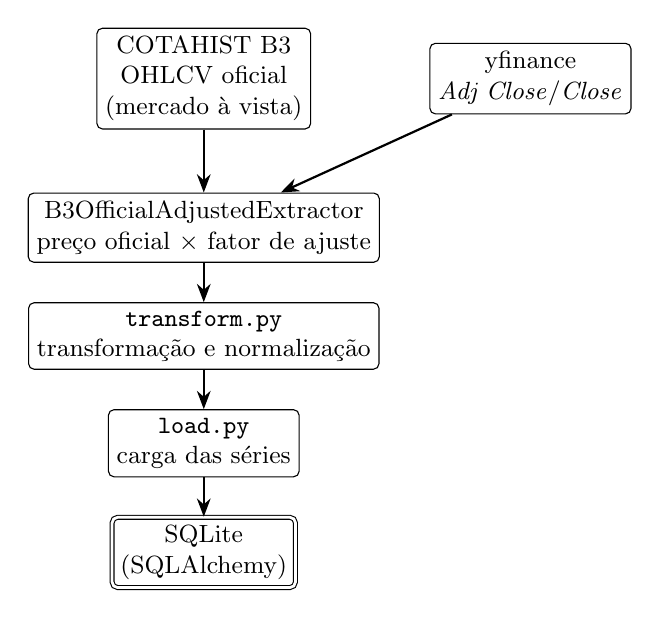
\begin{tikzpicture}[
  node distance=5mm and 15mm,
  box/.style={draw, rounded corners=2pt, minimum height=7mm, align=center, inner sep=3pt, font=\small},
  db/.style={box, double, double distance=1pt},
  arr/.style={-Stealth, thick},
]
\node[box] (cotahist) {COTAHIST B3\\OHLCV oficial\\(mercado à vista)};
\node[box, right=of cotahist] (yf) {yfinance\\\textit{Adj Close}/\textit{Close}};
\node[box, below=8mm of cotahist] (extr) {B3OfficialAdjustedExtractor\\preço oficial $\times$ fator de ajuste};
\draw[arr] (cotahist) -- (extr);
\draw[arr] (yf) -- (extr);
\node[box, below=of extr] (trans) {\texttt{transform.py}\\transformação e normalização};
\node[box, below=of trans] (load) {\texttt{load.py}\\carga das séries};
\node[db, below=of load] (sqlite) {SQLite\\(SQLAlchemy)};
\draw[arr] (extr) -- (trans);
\draw[arr] (trans) -- (load);
\draw[arr] (load) -- (sqlite);
\end{tikzpicture}
\caption{Fluxo do pipeline de dados científico: preço oficial da B3 (COTAHIST) combinado ao fator de ajuste por proventos do \texttt{yfinance}, seguido de transformação, carga e persistência em SQLite.}
\label{fig:pipeline}
\end{figure}

A série de preço científica de referência (\texttt{H\_real}) corresponde ao ativo PETR4.SA, com 1519 sessões no intervalo de 2018-01-12 a 2024-02-28, cobrindo 2649 barras oficiais.

O calendário de negociação é modelado pela classe \texttt{B3Calendar} (\texttt{src/backtesting/b3\_calendar.py}), que aplica as regras históricas de feriados da B3 e reproduz as 2649 sessões oficiais. A versão anterior do calendário apresentava divergências em datas específicas (feriados do estado de São Paulo, fim de ano e o feriado de 20 de novembro), corrigidas na versão atual.

% Fonte: dashboard/market_base_api.py; scripts/continuous_replay_data.py; scripts/replay_multiasset.py; DP-27.
O caminho multiativos utiliza uma base de mercado local dos cinco ativos (DP-27), mantida por \texttt{dashboard/market\_base\_api.py}, que separa duas representações por sessão: o OHLCV bruto (RAW) do COTAHIST, empregado na marcação a mercado e na execução simulada, e o fator de ajuste do Yahoo Finance, empregado apenas no cálculo dos indicadores e dos sinais. Para o Replay Contínuo, \texttt{scripts/continuous\_replay\_data.py} congela essa base em um \textit{bundle} próprio da campanha (\texttt{inputs/market.json} e \texttt{inputs/manifest.json}), com o \textit{hash} SHA-256 dos arquivos e o instante de aquisição; os fatores de ajuste foram adquiridos depois do período e, portanto, não constituem uma representação \textit{point-in-time}.

\section{Camada de Persistência}

A persistência das séries é implementada no módulo \texttt{src/db}, composto pela configuração de conexão (\texttt{connection.py}) e pela definição do esquema relacional (\texttt{models.py}). O acesso é feito por SQLAlchemy; o endereço do banco é configurável (\texttt{src/config.py}), com SQLite como valor padrão.

% Fonte: dashboard/manual_portfolio_api.py (SCHEMA, connect, append, replay, batch).
As carteiras simuladas utilizam um livro contábil distinto, implementado em \texttt{dashboard/manual\_portfolio\_api.py} (identidade \texttt{HFL-MANUAL-PORTFOLIO-V1}). Cada criação de carteira, operação, provento recebido ou recibo de decisão é gravado como um evento imutável em uma tabela SQLite com gatilhos que recusam \texttt{UPDATE} e \texttt{DELETE}. Cada evento armazena o \textit{hash} do evento anterior da mesma carteira, formando uma cadeia verificada a cada leitura; cada comando possui identificador único, o que torna a repetição de uma gravação idempotente. As escritas usam \texttt{BEGIN IMMEDIATE} e \texttt{synchronous=FULL}. Posições, caixa e base de custo não são armazenados como saldos: são recalculados a cada leitura pela reprodução ordenada dos eventos (\textit{replay}). Valores monetários e quantidades são tratados com \texttt{Decimal} e arredondados a centavos pelo núcleo contábil reutilizado de \texttt{scripts/multiasset\_portfolio.py}.

\section{Indicadores e Estratégias}

Os indicadores técnicos são implementados no módulo \texttt{src/indicators}: médias móveis simples (\texttt{sma.py}), Bandas de Bollinger (\texttt{bollinger.py}), Índice de Força Relativa (\texttt{rsi.py}) e MACD (\texttt{macd.py}). O RSI segue a formulação canônica de Wilder.

As estratégias residem em \texttt{src/strategies}, com uma interface comum em \texttt{base.py}. O conjunto inclui \textit{Buy and Hold} (\texttt{buy\_and\_hold.py}), carteira igualmente ponderada (\texttt{equal\_weight.py}), cruzamento de médias móveis (\texttt{sma\_cross.py}), Bandas de Bollinger (\texttt{bollinger\_bands.py}), mínima variância (\texttt{min\_variance.py}) e o controle clássico da família de indicadores (\texttt{indicator\_family\_control.py}). Esse último combina SMA, Bandas de Bollinger, RSI e MACD em um escore discreto no conjunto $\{-1, 0, +1\}$, servindo de \textit{benchmark} clássico para a comparação com o sistema multiagente de ativo único.

No caminho multiativos, as carteiras de referência reutilizam esses componentes por adaptadores: \texttt{dashboard/rule\_portfolios.py} aplica \texttt{sma\_cross.py} (50/200) e \texttt{bollinger\_bands.py} (20 períodos, 2 desvios) a parcelas independentes de 20\% do capital por ativo, e as carteiras de pesos iguais e de mínima variância utilizam as classes \texttt{EqualWeightPortfolio} e \texttt{MinVariancePortfolio} de \texttt{src/backtesting/portfolio.py} (Seção~\ref{sec:arq-replay}).

\section{Motor de Backtesting}

O motor de \textit{backtesting} é implementado em \texttt{src/backtesting} e centraliza a simulação de carteiras, o cálculo de métricas de desempenho e a incorporação de custos. O módulo \texttt{engine.py} conduz a simulação, \texttt{portfolio.py} modela a carteira, \texttt{costs.py} aplica custos de transação e \texttt{metrics.py} concentra as métricas de risco e retorno. O calendário de negociação (\texttt{b3\_calendar.py}) é utilizado pelo motor para alinhar as decisões às sessões oficiais. A integração com o sistema multiagente de ativo único é realizada por meio de \texttt{agent\_engine.py} e \texttt{daily\_agent.py}, que conectam as decisões produzidas pelos agentes à execução simulada, e por \texttt{arena.py}, que organiza a comparação entre estratégias.

A métrica primária de avaliação do sistema multiagente (Sharpe Ratio) é definida de forma congelada em \texttt{src/backtesting/metrics.py}, sob o identificador \texttt{H2\_SCIENTIFIC\_SHARPE\_DEFINITION\_V1}, cuja especificação é detalhada no Capítulo~\ref{cha:metodologia}.

O Replay Contínuo multiativos não utiliza \texttt{engine.py}: suas seis carteiras evoluem no livro de eventos descrito na seção anterior, com execução, custos e proventos aplicados pelos módulos da aplicação (Seção~\ref{sec:arq-relogio}). Do motor de \textit{backtesting}, reutilizam-se o calendário B3 e as classes de alocação de \texttt{portfolio.py}.

\section{Sistema Multiagente de Ativo Único}
\label{sec:arq-ativo-unico}

A lógica de decisão de ativo único do Hedge-fund-lab é modelada como um sistema multiagente coordenado pelo LangGraph, no módulo \texttt{src/agents}. O grafo de decisão é linear e acíclico: os agentes são executados em sequência, sem debate cíclico nem reavaliação iterativa. Cada nó do grafo corresponde a um papel especializado, e as arestas definem a ordem de execução entre eles.

Os papéis especializados são três. O agente de análise técnica (\texttt{technical\_analyst.py}) interpreta os indicadores quantitativos e emite uma recomendação inicial. O agente de gestão de risco (\texttt{risk\_manager.py}), amparado por um contrato de risco (\texttt{risk\_contract.py}), avalia a exposição e pode restringir a decisão. O agente de gestão de portfólio (\texttt{portfolio\_manager.py}) consolida as análises e define a decisão final. Na configuração científica, a direção da decisão é determinada pelo comitê e a exposição é atribuída por peso-alvo determinístico, sem dimensionamento dinâmico de posição pelo gestor de portfólio; o modo legado de dimensionamento por confiança permanece no código apenas como alternativa experimental.

O estado compartilhado do grafo é definido em \texttt{state.py}; as features e sua semântica, em \texttt{features.py} e \texttt{feature\_semantics.py}; a evidência técnica apresentada aos agentes, em \texttt{technical\_evidence.py}; e os \textit{prompts} de análise técnica, em \texttt{technical\_prompt\_v4.py} e \texttt{technical\_prompt\_v5.py}. A comunicação com o modelo de linguagem é encapsulada em \texttt{llm\_client.py}, com rastreamento das chamadas em \texttt{llm\_trace.py}. Cada participante do comitê é representado em \texttt{participant.py}.

O método de decisão é o \textit{self-consistency}, em que múltiplos analistas votam e a decisão consolidada exige um limiar de consenso com voto obrigatório de todos os participantes. A configuração congelada desses parâmetros é apresentada no Capítulo~\ref{cha:metodologia}.

A Figura~\ref{fig:grafo-langgraph} representa o grafo de decisão implementado em \texttt{src/agents/graph.py}: os agentes são executados em sequência linear, e a aresta condicional após o gestor de risco só encaminha a decisão ao gestor de portfólio quando o veredito consolidado é \texttt{APROVADO}.

\begin{figure}[htbp]
\centering
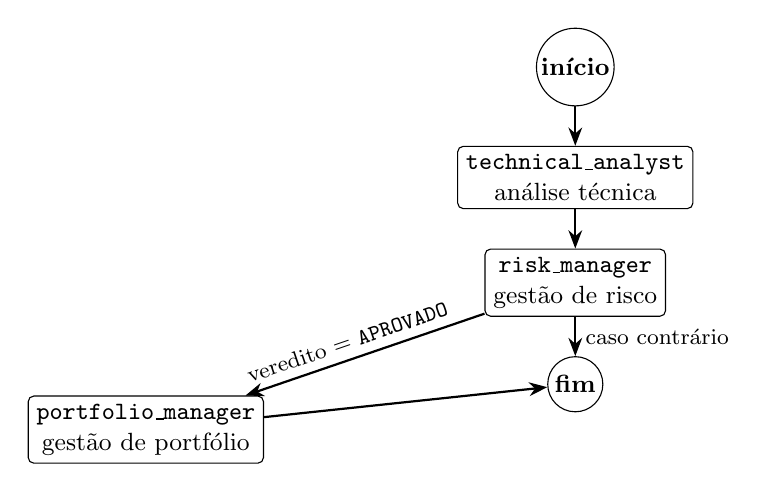
\begin{tikzpicture}[
  node distance=5mm,
  box/.style={draw, rounded corners=2pt, minimum height=7mm, align=center, inner sep=3pt, font=\small},
  term/.style={draw, circle, minimum size=7mm, align=center, font=\small\bfseries, inner sep=1pt},
  arr/.style={-Stealth, thick},
]
\node[term] (start) {início};
\node[box, below=of start] (ta) {\texttt{technical\_analyst}\\análise técnica};
\node[box, below=of ta] (rm) {\texttt{risk\_manager}\\gestão de risco};
\node[box, below left=10mm and 28mm of rm] (pm) {\texttt{portfolio\_manager}\\gestão de portfólio};
\node[term, below=of rm] (end) {fim};
\draw[arr] (start) -- (ta);
\draw[arr] (ta) -- (rm);
\draw[arr] (rm) -- node[above, sloped, pos=0.55, font=\footnotesize] {veredito = \texttt{APROVADO}} (pm);
\draw[arr] (pm) -- (end);
\draw[arr] (rm) -- node[right, font=\footnotesize] {caso contrário} (end);
\end{tikzpicture}
\caption{Grafo de decisão do sistema multiagente de ativo único (LangGraph): sequência linear \texttt{technical\_analyst} $\rightarrow$ \texttt{risk\_manager}, com aresta condicional que encaminha ao \texttt{portfolio\_manager} apenas quando o veredito é \texttt{APROVADO}.}
\label{fig:grafo-langgraph}
\end{figure}

O grafo (\texttt{build\_graph}) é utilizado pelos participantes da arena experimental (\texttt{src/agents/participant.py}) e pelos executores de ativo único (\texttt{scripts/run\_agent\_backtest.py}, \texttt{scripts/run\_agent\_daily.py}). O participante recusa universos com mais de um ativo, e seu estado mantém posição escalar, caixa e patrimônio de um único papel. Por essa razão, a carteira multiativos não instancia o grafo: reutiliza o nó do comitê técnico e os esquemas de resposta de \texttt{src/agents}, mas substitui o gestor de risco e o gestor de portfólio por papéis próprios, descritos a seguir.

\section{Carteira Multiagente Multiativos}
\label{sec:arq-multiativos}

% Fonte: scripts/multiasset_radar.py (technical_input, committee, RISK_PROMPT);
% dashboard/wallet_manager_api.py (PROMPT, Proposal, compile_proposal);
% dashboard/auction_orders.py (plan); scripts/continuous_replay.py (execute).
A carteira multiativos opera um universo fixo de cinco ações da B3 (BBAS3, ITUB4, PETR4, VALE3 e WEGE3) com caixa compartilhado. A decisão de cada pregão é organizada em quatro etapas: um comitê de analistas por ativo, um analista de risco por ativo, um gestor global da carteira e um compilador determinístico da proposta. Na configuração utilizada no Replay Contínuo, todos os papéis baseados em modelo de linguagem empregam \texttt{gemini-3.8-flash}, com temperatura 1,0, nível de raciocínio baixo e até 8.192 \textit{tokens} de saída. A Figura~\ref{fig:fluxo-multiativos} resume o fluxo de um pregão.

\subsection{Comitê de analistas por ativo}

O comitê por ativo é implementado no Radar multiativos (\texttt{scripts/multiasset\_radar.py}, identidade \texttt{HFL-MULTIASSET-RADAR-V1}). A preparação da entrada (\texttt{technical\_input}) valida o OHLCV, exige histórico mínimo de 200 sessões, verifica a igualdade entre as datas das barras e a grade do \texttt{B3Calendar}, recusa sessões sem negociação e calcula, por meio do \texttt{DataTransformer} do pipeline, oito features adimensionais (\texttt{rsi}, \texttt{sma50\_gap}, \texttt{sma200\_gap}, \texttt{bb\_upper\_gap}, \texttt{bb\_lower\_gap}, \texttt{bb\_width}, \texttt{macd\_ratio} e \texttt{macd\_signal\_ratio}), além da volatilidade anualizada dos últimos 21 retornos diários.

A função \texttt{committee} reutiliza o nó de comitê técnico de \texttt{src/agents/technical\_analyst.py} com cinco analistas, \textit{prompt} técnico versão 5, sementes 10001 a 10005, limiar de consenso 0,6 e exigência de voto válido de todos os analistas. Cada voto é uma resposta estruturada com sinal (COMPRA, VENDA ou MANTER), confiança autodeclarada e códigos de evidência restritos ao vocabulário permitido para as features recebidas (\texttt{src/agents/technical\_evidence.py}). Com limiar 0,6, o consenso exige ao menos três votos no mesmo sinal; na ausência de consenso, o sinal encaminhado é MANTER com confiança nula. Os analistas recebem apenas as features do ativo: posições da carteira e dia-alvo não entram em seus \textit{prompts}.

\subsection{Analista de risco por ativo}

O risco é avaliado por ativo, sem conhecimento da carteira. Quando a volatilidade anualizada de 21 dias supera 50\%, uma regra determinística (\texttt{HARD\_ASSET\_VOLATILITY\_RULE}) emite o veredito \texttt{VETADO} sem chamada ao modelo. Caso contrário, uma chamada consultiva (\texttt{ADVISORY\_LLM}) recebe o sinal consolidado, as features e a volatilidade, e devolve \texttt{APROVADO} ou \texttt{VETADO} no esquema \texttt{RiskVerdict} de \texttt{src/agents/state.py}. O \textit{prompt} de risco proíbe inventar concentração, caixa, posições ou \textit{drawdown} da carteira; o risco agregado da carteira é registrado explicitamente como não avaliado (\texttt{NOT\_EVALUATED}). Na versão original, a recomendação encaminhada ao gestor é o sinal técnico quando o risco aprova e MANTER quando veta.

\subsection{Gestor global da carteira}

O gestor da carteira é implementado em \texttt{dashboard/wallet\_manager\_api.py} (identidade \texttt{HFL-WALLET-MANAGER-V1}). Ele recebe um contexto canônico com a carteira (posições e caixa), a sessão de referência, o dia-alvo, os preços de fechamento RAW da sessão de referência, os pareceres dos cinco ativos e a taxa de custo declarada, e devolve uma única resposta coordenada para o capital compartilhado. O esquema Pydantic \texttt{Proposal} exige um resumo, uma lista de ações e uma lista de riscos; cada ação contém \textit{ticker}, lado (\texttt{BUY}, \texttt{SELL} ou \texttt{HOLD}), quantidade inteira a movimentar e justificativa. O \textit{prompt} exige exatamente uma ação por ativo, trata os pareceres como dados e não como instruções, proíbe crédito, venda a descoberto e frações, e permite manter caixa. O transporte durável, o diário de chamadas e a validação de esquema são reutilizados do gestor global consultivo (\texttt{scripts/run\_global\_pm\_v2.py}) por vinculação de módulo (\texttt{pilot\_paper.bind}), sem alteração das fontes seladas desse gestor.

\subsection{Compilador determinístico da proposta}

A resposta do gestor não é aplicada diretamente. A função \texttt{compile\_proposal} valida a resposta contra o esquema e aplica, em ordem (vendas, manutenções, compras), as regras: universo completo e sem \textit{tickers} repetidos; \texttt{HOLD} com quantidade zero; compra apenas com recomendação COMPRA e risco \texttt{APROVADO}; venda apenas com recomendação VENDA e risco \texttt{APROVADO}; venda limitada à posição; caixa nunca negativo após custos. O resultado é uma tabela antes/depois por ativo (quantidade, valor e peso), a lista de operações e o patrimônio projetado. Na versão original, qualquer violação interrompe a compilação, e o pregão é registrado sem operações (Seção~\ref{sec:arq-replay}); as versões posteriores alteram esse comportamento (Seção~\ref{sec:arq-evolucao}).

\subsection{Planejamento da execução e livro}

A cesta compilada é convertida em operações por \texttt{dashboard/auction\_orders.py::plan}. As vendas são processadas primeiro; se o caixa resultante não cobrir as compras, todas as compras são reduzidas pelo mesmo fator em ações inteiras e, persistindo a insuficiência, a maior compra perde uma ação por vez até caber. Um ativo sem preço oficial não é executado, sem substituição por outro preço. A origem de cada operação registra quatro preços (decisão, prévia, aprovação e leilão), o que permite medir o custo de implementação. As operações são gravadas no livro de eventos em uma única transação, mediante prévia e confirmação por \textit{token} (\texttt{manual\_portfolio\_api.batch}).

\begin{figure}[htbp]
\centering
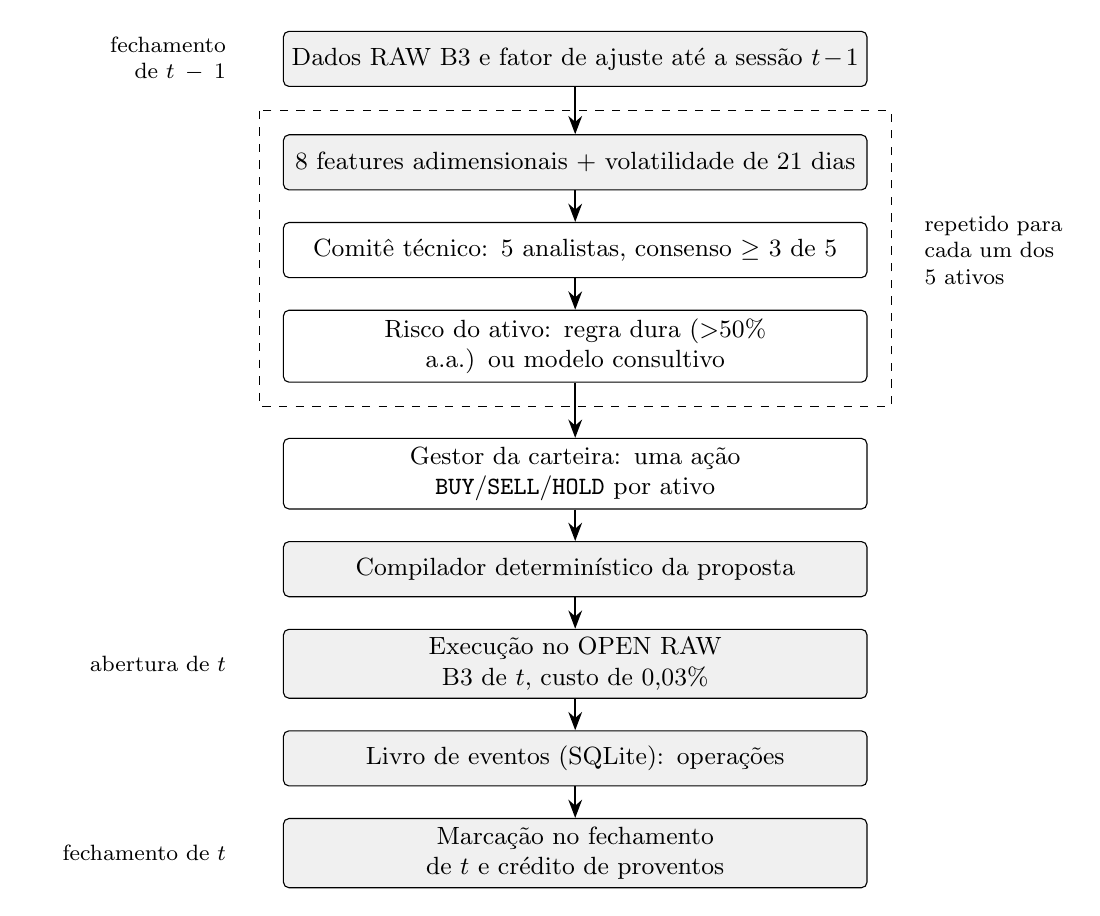
\begin{tikzpicture}[
  node distance=4mm,
  box/.style={draw, rounded corners=2pt, minimum height=7mm, text width=7.2cm, align=center, inner sep=3pt, font=\small},
  det/.style={box, fill=black!6},
  note/.style={font=\footnotesize, align=right, text width=2.4cm},
  arr/.style={-Stealth, thick},
]
\node[det] (dados) {Dados RAW B3 e fator de ajuste até a sessão $t-1$};
\node[det, below=6mm of dados] (feat) {8 features adimensionais + volatilidade de 21 dias};
\node[box, below=of feat] (comite) {Comitê técnico: 5 analistas, consenso $\geq$ 3 de 5};
\node[box, below=of comite] (risco) {Risco do ativo: regra dura ($>$50\% a.a.) ou modelo consultivo};
\node[box, below=7mm of risco] (gestor) {Gestor da carteira: uma ação \texttt{BUY}/\texttt{SELL}/\texttt{HOLD} por ativo};
\node[det, below=of gestor] (comp) {Compilador determinístico da proposta};
\node[det, below=of comp] (exec) {Execução no OPEN RAW B3 de $t$, custo de 0,03\%};
\node[det, below=of exec] (livro) {Livro de eventos (SQLite): operações};
\node[det, below=of livro] (marca) {Marcação no fechamento de $t$ e crédito de proventos};
\draw[arr] (dados) -- (feat);
\draw[arr] (feat) -- (comite);
\draw[arr] (comite) -- (risco);
\draw[arr] (risco) -- (gestor);
\draw[arr] (gestor) -- (comp);
\draw[arr] (comp) -- (exec);
\draw[arr] (exec) -- (livro);
\draw[arr] (livro) -- (marca);
\draw[dashed] ([xshift=-3mm, yshift=3mm]feat.north west) rectangle ([xshift=3mm, yshift=-3mm]risco.south east);
\node[font=\footnotesize, align=left, anchor=west] at ([xshift=6mm]comite.east) {repetido para\\cada um dos\\5 ativos};
\node[note, anchor=east] at ([xshift=-6mm]dados.west) {fechamento\\de $t-1$};
\node[note, anchor=east] at ([xshift=-6mm]exec.west) {abertura de $t$};
\node[note, anchor=east] at ([xshift=-6mm]marca.west) {fechamento de $t$};
\end{tikzpicture}
\caption{Fluxo de um pregão $t$ na carteira multiagente multiativos. Caixas sombreadas são etapas determinísticas; caixas brancas envolvem chamadas ao modelo de linguagem (a etapa de risco apenas quando a regra dura não se aplica). O retângulo tracejado indica as etapas executadas por ativo.}
\label{fig:fluxo-multiativos}
\end{figure}

\section{Relógio Causal do Pregão}
\label{sec:arq-relogio}

% Fonte: scripts/replay_multiasset.py (prepare, LIMITATIONS); scripts/continuous_replay*.py
% (execute, preflight); dashboard/auction_orders.py (plan); dashboard/dividends_api.py (JCP_NET).
O tratamento temporal de cada pregão-alvo $t$ separa a informação disponível para a decisão da informação usada para executar e avaliar:

\begin{enumerate}
  \item \textbf{Decisão com dados até $t-1$.} A entrada de cada ativo é construída por \texttt{scripts/replay\_multiasset.py} a partir das barras compreendidas entre 450 dias corridos antes da sessão de referência e a própria sessão de referência, que é o pregão imediatamente anterior a $t$. O aquecimento dos indicadores não cria patrimônio anterior ao início da campanha.
  \item \textbf{Aprovação hipotética às 09:00 de $t$.} No replay, a cesta compilada é considerada aprovada antes da abertura, sem a prévia com cotação atrasada, o alerta de tese velha e as tentativas das 12:00 e 16:00 do ciclo diário (Seção~\ref{sec:arq-operacao-diaria}).
  \item \textbf{Execução no OPEN RAW B3 de $t$.} O preço de execução é a abertura oficial bruta do COTAHIST (campo PREABE), usada como aproximação diária do leilão de abertura, sem \textit{spread}, impacto, livro de ofertas ou liquidação em D+2. Cada operação posterior à entrada paga custo de 0,03\% sobre o valor bruto; não há custo fixo nem lote mínimo de bolsa.
  \item \textbf{Marcação no fechamento de $t$.} As carteiras são marcadas ao fechamento RAW B3 de $t$. Os proventos seguem a DP-30: o direito é determinado pela posição na data-com, o JCP é creditado líquido de 15\% de imposto (\texttt{JCP\_NET} em \texttt{dashboard/dividends\_api.py}) e o valor só entra no caixa na data de pagamento; entre as duas datas, aparece como recebível, que compõe o patrimônio mas não o caixa disponível para compras. O caixa não é remunerado.
\end{enumerate}

Os sinais das carteiras de referência utilizam o fechamento B3 multiplicado pelo fator de ajuste; operações e patrimônio de todas as carteiras utilizam preços RAW. Essa separação impede que um preço ajustado retroativamente altere a contabilidade.

A proteção contra antecipação de informação (\textit{look-ahead}) atua em três pontos. Primeiro, a entrada é truncada na sessão de referência; o verificador do primeiro ensaio (\texttt{tests/check\_multiasset\_replay.py}) adultera barras futuras e confere que as entradas permanecem idênticas. Segundo, o \textit{preflight} das versões v2 e v3, executado sob bloqueio de rede (\texttt{no\_network()}), percorre todas as entradas da campanha e interrompe a execução com \texttt{decision\_input\_lookahead} se alguma sessão de entrada for igual ou posterior ao dia-alvo. Terceiro, imediatamente antes de cada requisição HTTP, a entrada é relida e comparada com a versão registrada; qualquer diferença interrompe a campanha (\texttt{input\_changed\_before\_transport}), e o mesmo ocorre com o contexto do gestor (\texttt{manager\_context\_changed\_before\_transport}). Esses controles garantem a causalidade dos dados entregues aos agentes, mas não eliminam a possibilidade de o modelo conhecer o período por seu treinamento; essa limitação é tratada no Capítulo~\ref{cha:metodologia}.

\section{Arquitetura do Replay Contínuo}
\label{sec:arq-replay}

% Fonte: scripts/continuous_replay.py, continuous_replay_v2.py, continuous_replay_v3.py,
% continuous_replay_runtime.py, continuous_replay_dividends.py, export_continuous_replay*.py,
% build_replay_explorer.py, publish_replay.py, dashboard/server.py (_serve_replay).
O Replay Contínuo Abril--Novembro de 2026 reconstitui, em uma única trajetória sem reinício, 153 pregões da B3 (06/04/2026 a 12/11/2026) para seis carteiras independentes de R\$ 100.000,00: a carteira Multiagentes e cinco carteiras de referência determinísticas. É uma reconstrução retrospectiva, produzida após o fim do período, autorizada como extensão exploratória (DP-37). O desenho experimental é apresentado no Capítulo~\ref{cha:metodologia} e os resultados, no Capítulo~\ref{cha:resultados}; esta seção descreve o mecanismo que os produz.

\subsection{Runners, identidades e isolamento}

Cada geração possui um executor próprio: \texttt{scripts/continuous\_replay.py} (identidade \texttt{HFL-CONTINUOUS-EXPLORATORY-REPLAY-V1}), \texttt{scripts/continuous\_replay\_v2.py} (\texttt{-V2}) e \texttt{scripts/continuous\_replay\_v3.py} (\texttt{-V3}), cada um com raiz de armazenamento, livro, orçamento e pacote exportado próprios. As versões v2 e v3 consomem as mesmas entradas congeladas da v1, conferindo o \textit{hash} do \textit{bundle} de mercado antes do uso, e reutilizam contabilidade, livro, planejador de execução, transporte e orçamento por vinculação de módulo (\texttt{pilot\_paper.bind}), sem editar as fontes das versões anteriores.

No início de cada execução, o executor monta um manifesto da campanha com a identidade, o modo (inferência real ou teste \textit{offline}), as sessões, as estratégias, as políticas de referência, o teto de orçamento e os \textit{hashes} SHA-256 de todas as fontes utilizadas. Se já existir um manifesto diferente na raiz, a execução é recusada (\texttt{campaign\_identity\_changed}), o que impede retomar uma campanha com código ou dados distintos dos que a iniciaram. A v1 copia ainda os módulos de livro, proventos e regras para uma pasta imutável da campanha (\texttt{engine/}) e confere, por \textit{hash}, que as estratégias SMA/Bollinger e de portfólio efetivamente importadas coincidem com essas cópias. Um \textit{lock} exclusivo impede dois executores simultâneos sobre a mesma raiz.

\subsection{Carteiras iniciais e referências pré-calculadas}

A função \texttt{initialize} cria as seis carteiras no livro em uma única transação, cada uma com a mesma cesta inicial (DP-20): 20\% do capital por ativo em ações inteiras, ao fechamento da sessão anterior ao primeiro pregão, com custo zero e sem alegação de execução a mercado. Uma falha durante a criação não deixa carteiras parciais.

As cinco referências são calculadas integralmente pela função \texttt{references} antes do laço de inferência, e podem ser produzidas isoladamente (\texttt{--references-only}), sem chamadas ao modelo; nas versões v2 e v3, esse modo executa sob bloqueio de rede (\texttt{no\_network()}). O \textit{Buy \& Hold} mantém a cesta inicial sem rebalanceamento. SMA 50/200 e Bollinger 20/2 avançam por \texttt{rule\_portfolios.advance\_wallet}, decidindo no fechamento de $t-1$ e executando na abertura de $t$. Pesos iguais e mínima variância (janela de 252 retornos, somente posições compradas) são recalculados a cada 63 pregões; os pesos são convertidos em quantidades inteiras à abertura e executados pelo mesmo planejador da carteira Multiagentes. No otimizador SLSQP da mínima variância, a função-objetivo é dividida por um escalar positivo (a maior variância da diagonal), o que preserva o minimizador e as restrições; os pesos, a janela, o resultado do otimizador e eventual recurso aos pesos iguais ficam registrados no recibo de decisão. Em todas as referências, os proventos permanecem em caixa, sem reinvestimento. A igualdade das referências entre as três campanhas é conferida por auditoria posterior (\texttt{scripts/audit\_replay\_v2\_comparison.py} e \texttt{scripts/audit\_replay\_v3\_comparison.py}).

\subsection{Laço diário e semântica \textit{fail-closed}}

Para cada pregão, o executor grava artefatos intermediários selados na pasta da sessão, nesta ordem: o estado das carteiras antes do pregão (\texttt{before.json}), após o crédito dos proventos pagos até a referência; o resultado do comitê de cada ativo (\texttt{result.json} ou \texttt{failure.json}), com a entrada e o diário de chamadas; o contexto e a proposta compilada do gestor (\texttt{context.json}, \texttt{proposal.json}); o plano de execução (\texttt{execution.json}); e o fechamento do dia (\texttt{day.json}), que contém a marcação das seis carteiras. A existência de cada artefato faz com que a etapa correspondente seja reaproveitada em vez de reexecutada, de modo que uma interrupção é retomada no mesmo ponto, sem nova chamada ao modelo para etapas já concluídas.

Quando o comitê de algum ativo não se completa ou a proposta do gestor não pode ser compilada, o pregão é registrado como \texttt{NO\_ANALYSIS}: nenhuma operação é gravada, as posições vigentes são preservadas, as seis carteiras são marcadas normalmente e a campanha prossegue. Votos parciais recebidos permanecem registrados, e nenhuma decisão é fabricada para preencher a lacuna. Erros de integridade do diário ou do orçamento, ao contrário, interrompem a campanha.

\subsection{Orçamento e rastreamento das chamadas}

O controle de custo é implementado em \texttt{scripts/continuous\_replay\_runtime.py} e é independente da estratégia. Cada campanha possui um teto agregado único de US\$ 34,78, que inclui tentativas repetidas, chamadas em andamento e respostas sem uso conhecido. Antes de cada tentativa HTTP, uma reserva é gravada em SQLite com \texttt{synchronous=FULL}: US\$ 0,110592 por chamada de analista ou de risco e US\$ 0,159744 por chamada do gestor, valores calculados pelos limites de \textit{bytes} de entrada e \textit{tokens} de saída às tarifas mais altas anunciadas. Se a reserva ultrapassar o teto, a campanha é interrompida. Ao receber a resposta, o custo é estimado a partir dos \textit{tokens} informados pelo provedor (US\$ 0,75 por milhão de \textit{tokens} de entrada e US\$ 3,75 por milhão de \textit{tokens} de saída e de raciocínio); sem uso válido, a reserva integral permanece contabilizada. A estimativa não substitui a fatura do provedor.

Cada chamada lógica admite no máximo duas tentativas físicas, apenas para falhas de transporte. Uma resposta já recebida e persistida é sempre reutilizada, inclusive após interrupção, e nunca solicitada novamente; esgotadas as duas tentativas, não há substituição automática. Esperas de reenvio superiores a 30 segundos e respostas que ecoem a credencial de acesso interrompem a execução. Cada comitê e cada gestor possuem um diário de chamadas (\texttt{CallBank}) com requisições, envelopes brutos e respostas validadas, exportado ao final como \texttt{provider\_journal.jsonl}. A auditoria do orçamento (\texttt{audit\_budget}, nos exportadores) reconstrói todas as tentativas, confere o \textit{hash} de cada envelope, recalcula o custo a partir dos \textit{tokens} e verifica que nenhuma chamada lógica teve mais de duas tentativas ou mais de uma resposta consumida.

\subsection{Exportação, pacotes selados e explorador de consulta}

Os exportadores (\texttt{scripts/export\_continuous\_replay.py}, \texttt{\_v2.py} e \texttt{\_v3.py}) leem os recibos já gravados, sem inferência nem alteração do livro, e produzem: \texttt{explorer.json} com as sessões, carteiras, pareceres e operações; \texttt{calls.json} com as chamadas arquivadas; tabelas CSV de patrimônio diário, operações, decisões, proventos e chamadas; uma página HTML autônoma com Chart.js embutido e um carregador das chamadas sob demanda (\texttt{calls-data.js}), gerados pelo próprio exportador nas versões v2 e v3 e por \texttt{scripts/build\_replay\_explorer.py} na v1; e um \texttt{manifest.json} selado com o \textit{hash} da exportação e o resultado da auditoria de orçamento. O conjunto é distribuído como um pacote ZIP.

A instalação no servidor é feita por \texttt{scripts/publish\_replay.py}, que aceita apenas o pacote cujo SHA-256 está fixado no código para cada versão (v1, v2 ou v3) e com a lista exata de membros esperada. Os arquivos são extraídos em área temporária, conferidos e promovidos por renomeação no mesmo volume; um destino existente só é aceito se seus arquivos coincidirem com o pacote, e dados diferentes nunca são sobrescritos. Cada versão ocupa um diretório próprio, preservando as anteriores.

A consulta é servida pelas rotas \texttt{/laboratory/replay/}, \texttt{/laboratory/replay/v2/} e \texttt{/laboratory/replay/v3/} de \texttt{dashboard/server.py}, somente com leitura: o servidor entrega apenas uma lista fechada de dez arquivos exportados, confina o caminho ao diretório da versão, comprime as respostas grandes sob demanda e não executa agentes nem operações. O explorador compara as curvas das seis carteiras e permite inspecionar, por carteira e pregão, posições, votos, pareceres de risco, decisões, operações, proventos e as chamadas arquivadas ao modelo. Os textos produzidos pelos modelos são apresentados como evidência preservada, não como fatos verificados.

\section{Evolução da Arquitetura entre Versões}
\label{sec:arq-evolucao}

% Fonte: scripts/continuous_replay_v2.py (constantes, LENTE_*, committee_v2, PROMPT_V2,
% compile_proposal_v2); scripts/continuous_replay_v3.py (constantes, _LENS_SUFFIX,
% committee_v3, PROMPT_V3, compute_position_memory, compile_proposal_v3).
As três gerações mantêm a mesma topologia de agentes por pregão --- cinco analistas por ativo, até um analista de risco por ativo e um gestor, no máximo 31 chamadas ---, o mesmo modelo e configuração de geração, as mesmas features, a mesma regra dura de volatilidade, o mesmo \textit{prompt} de risco e o mesmo esquema de resposta do gestor. Também são comuns a execução, os custos, os proventos, o orçamento e as cinco referências. Variam a composição do comitê, a regra de agregação e de veto, o contexto e as regras do gestor e o comportamento do compilador, conforme a Tabela~\ref{tab:evolucao-versoes}. Os resultados de cada versão são apresentados no Capítulo~\ref{cha:resultados}.

\begin{table}[htbp]
\centering
\caption{Diferenças arquiteturais entre as três gerações da carteira Multiagentes no Replay Contínuo.}
\label{tab:evolucao-versoes}
\small
\setlength{\tabcolsep}{4pt}
\begin{tabular}{>{\raggedright\arraybackslash}p{3.0cm} >{\raggedright\arraybackslash}p{3.8cm} >{\raggedright\arraybackslash}p{3.8cm} >{\raggedright\arraybackslash}p{4.0cm}}
\toprule
\textbf{Dimensão} & \textbf{v1} & \textbf{v2} & \textbf{v3} \\
\midrule
\textit{Prompt} dos analistas & Um único \textit{prompt} (v5) para os cinco & \textit{Prompt} base + 3 lentes (2 + 2 + 1) & \textit{Prompt} base + 5 lentes distintas \\
Travas sobre o consenso & Não & Não & Reversão de consensos 3--2 em extremos \\
Efeito do veto de risco & \texttt{VETADO} $\rightarrow$ MANTER & \texttt{VETADO} bloqueia só compras (R7) & Igual à v2 \\
Contexto do gestor & Carteira, preços e pareceres & Igual à v1 & Acrescenta memória de posição \\
\textit{Prompt} do gestor & Original & \texttt{PROMPT\_V2} (4 regras) & \texttt{PROMPT\_V3} (7 regras) \\
Compilador & Estrito: violação invalida o pregão & Ajusta e registra (\texttt{strict=False}) & Ajusta e registra (\texttt{strict=False}) \\
Limites de compra & Caixa disponível & Teto de 30\% e mínimo de R\$ 2.000 & Teto de 30\% (22\% em recomposição) e mínimo de R\$ 2.000 \\
Vendas parciais fora de VENDA & Não & \textit{Trim-to-Fund} & \textit{Trim-to-Fund} e \textit{Trim-on-Strength} \\
Limites de venda em VENDA & Posição & Posição & 45\% da posição por pregão e piso de 8\% \\
\bottomrule
\end{tabular}
\end{table}

\subsection{Versão v2}

A v2 acrescenta quatro intervenções, todas impostas tanto no \textit{prompt} do gestor (\texttt{PROMPT\_V2}) quanto no compilador (\texttt{compile\_proposal\_v2}):

\begin{itemize}
  \item \textbf{\textit{Trim-to-Fund}:} venda parcial de ativo com recomendação MANTER ou COMPRA, admitida quando o peso antes da operação supera 25\% do patrimônio, o peso projetado permanece em ao menos 15\% e a cesta contém uma compra válida ou o ativo já excede 30\%.
  \item \textbf{Teto de concentração e ordem mínima:} nenhuma compra pode levar o peso projetado do ativo acima de 30\% do patrimônio anterior à operação (\texttt{MAX\_ASSET\_WEIGHT}), nem ter valor bruto inferior a R\$ 2.000,00 (\texttt{MIN\_TRADE\_BRL}); vendas não têm valor mínimo.
  \item \textbf{Veto assimétrico (R7):} o veredito \texttt{VETADO} passa a bloquear apenas compras; se o consenso técnico for VENDA, a recomendação permanece VENDA sob veto (\texttt{committee\_v2}), permitindo reduzir ou zerar a posição.
  \item \textbf{Lentes analíticas:} cada analista recebe o \textit{prompt} técnico v5 acrescido de uma lente --- tendência estrutural (analistas 1 e 2), reversão por Bollinger e RSI (3 e 4) e regime de volatilidade como árbitro (5).
\end{itemize}

Além disso, o compilador deixa de invalidar o pregão diante de uma violação de regra: em modo não estrito, reduz a quantidade ou converte a ação em \texttt{HOLD} e registra cada ajuste com \textit{ticker}, lado e quantidade de origem e destino e o motivo (por exemplo, \texttt{MAX\_ASSET\_WEIGHT\_CAP}, \texttt{MIN\_TRADE\_BRL}, \texttt{TRIM\_WEIGHT\_AFTER\_FLOOR}). Violações estruturais --- universo incompleto ou com \textit{tickers} repetidos e quantidades inválidas --- continuam invalidando o pregão.

\subsection{Versão v3}

A v3 mantém as regras da v2 e acrescenta quatro grupos de mecanismos, parametrizados por constantes de \texttt{scripts/continuous\_replay\_v3.py} (Tabela~\ref{tab:constantes-v3}).

\begin{table}[htbp]
\centering
\caption{Constantes determinísticas da versão v3.}
\label{tab:constantes-v3}
\small
\begin{tabular}{l r p{6.4cm}}
\toprule
\textbf{Constante} & \textbf{Valor} & \textbf{Função} \\
\midrule
\texttt{MAX\_ASSET\_WEIGHT} & 0,30 & Teto de peso projetado em compra por COMPRA \\
\texttt{DIP\_REBALANCE\_MAX\_WEIGHT} & 0,22 & Teto de peso em compra de recomposição em MANTER \\
\texttt{MIN\_TRADE\_BRL} & 2.000,00 & Valor bruto mínimo de compra (R\$) \\
\texttt{CORE\_FLOOR\_WEIGHT} & 0,08 & Peso mínimo remanescente após venda técnica normal \\
\texttt{MAX\_NORMAL\_SELL\_FRACTION} & 0,45 & Fração máxima da posição vendida por pregão \\
\texttt{ANTI\_WHIPSAW\_COOLDOWN\_SESSIONS} & 8 & Janela contra recompra mais cara (pregões) \\
\texttt{CASH\_DRAG\_THRESHOLD} & 0,25 & Caixa/patrimônio que habilita a recomposição \\
\texttt{STRENGTH\_TRIM\_MAX\_FRACTION} & 0,35 & Fração máxima de uma realização em força \\
\texttt{STRENGTH\_TRIM\_MIN\_WEIGHT\_AFTER} & 0,12 & Peso mínimo após realização em força \\
\texttt{TRIM\_MIN\_WEIGHT\_BEFORE}/\texttt{\_AFTER} & 0,25/0,15 & Limites do \textit{Trim-to-Fund}, herdados da v2 \\
\bottomrule
\end{tabular}
\end{table}

\begin{itemize}
  \item \textbf{Cinco lentes especialistas e travas de extremo.} Cada analista recebe uma lente única: Bandas de Bollinger, exaustão por RSI e MACD, valor relativo à média de 50 pregões, estrutura de longo prazo pela média de 200 pregões e assimetria entre o espaço até as bandas superior e inferior. Cada lente explicita faixas em que determinado sinal é proibido. Em \texttt{committee\_v3}, duas travas atuam apenas sobre consensos de exatamente três votos: \texttt{ANTI\_BOTTOM\_SELL\_GUARD} reverte VENDA para MANTER quando o RSI é inferior a 40 ou \texttt{bb\_lower\_gap} é inferior a 0,035, desde que \texttt{sma200\_gap} seja superior a $-0{,}08$; \texttt{ANTI\_TOP\_CHASE\_GUARD} reverte COMPRA para MANTER quando o RSI é superior a 62 ou \texttt{bb\_upper\_gap} é superior a $-0{,}02$.
  \item \textbf{Memória de posição, piso núcleo, venda escalonada e \textit{anti-whipsaw}.} A função \texttt{compute\_position\_memory} reconstrói do livro, por ativo, a quantidade, o preço médio de compra, o retorno não realizado, a sessão e o preço da última venda e os pregões decorridos desde ela, e inclui esses campos no contexto do gestor. Em venda técnica normal (VENDA com risco aprovado), o compilador limita a quantidade a 45\% da posição, arredondada para cima, e preserva peso remanescente de ao menos 8\% (ajuste \texttt{CORE\_FLOOR\_STEP\_SELL}); a saída integral fica restrita à venda sob veto (R7). É recusada a compra de ativo vendido nos últimos oito pregões a preço superior ao da última venda (\texttt{ANTI\_WHIPSAW\_HIGHER\_REBUY}).
  \item \textbf{\textit{Trim-on-Strength} e \textit{Trim-to-Fund}.} Além do \textit{Trim-to-Fund} da v2, admite-se a realização parcial em força de ativo em MANTER ou COMPRA quando ele está esticado (RSI $\geq$ 63 ou \texttt{bb\_upper\_gap} $\geq -0{,}02$), em lucro de ao menos 2\% sobre o preço médio e com peso acima de 14\%, limitada a 35\% da posição e a peso remanescente de 12\%, sem exigir compra na cesta.
  \item \textbf{Recomposição contra o arrasto de caixa (\textit{Dip-Rebalance}).} Quando o caixa do início do pregão supera 25\% do patrimônio, admite-se compra de ativo em MANTER com risco aprovado e em desconto (\texttt{sma50\_gap} negativo com RSI de até 46, ou \texttt{bb\_lower\_gap} de até 0,04), sujeita ao teto de 22\%, à ordem mínima e à regra \textit{anti-whipsaw}.
\end{itemize}

As regras de ambas as versões foram formuladas após a observação das campanhas anteriores sobre o mesmo período. Por isso, a evolução descrita nesta seção é tratada como iteração de engenharia dentro da amostra, e não como validação independente das regras; essa restrição é discutida nos Capítulos~\ref{cha:metodologia} e~\ref{cha:resultados}. A qualificação de cada versão antes da execução paga foi feita com respostas simuladas do modelo e rede bloqueada (\texttt{tests/check\_continuous\_replay\_v2.py} e \texttt{tests/check\_continuous\_replay\_v3.py}); essas verificações atestam o funcionamento do mecanismo e não constituem desempenho dos agentes.

\section{Operação Diária}
\label{sec:arq-operacao-diaria}

% Fonte: dashboard/daily_cycle.py (docstring, SLOTS, CAP_USD, windows, manager, close_day);
% dashboard/auction_orders.py (first_auction, execution_slot); Dockerfile; railway.json; DP-33/34/35.
Fora do replay, a mesma carteira multiativos é operada diariamente sobre dados correntes, em regime de simulação sem capital real e sem envio de ordens a corretoras. O ciclo autônomo (DP-34) é implementado em \texttt{dashboard/daily\_cycle.py} (identidade \texttt{HFL-DAILY-CYCLE-V1}) e executa dentro do processo do servidor quando habilitado por variável de ambiente. Em cada pregão da B3 há tentativas às 09:00, 12:00 e 16:00 (horário de São Paulo); uma tentativa posterior só ocorre se a anterior não tiver encerrado o dia.

Cada tentativa percorre, chamando as mesmas funções usadas pela interface, as etapas: atualização da base de mercado; abertura de uma análise com dia-alvo no pregão corrente e dados até o último pregão encerrado e publicado; preparação dos dados; comitês por ativo; contexto, \textit{preflight} e chamada do gestor; prévia com cotação atrasada; e aprovação automática, exceto quando o \textit{backend} emite alerta de tese velha, caso em que a cesta aguarda revisão humana. As reservas de custo do dia são limitadas a US\$ 4,00, somando analistas, gestor e todas as tentativas. Cada tentativa gera um registro selado e imutável, e o dia é encerrado em um de três estados: concluído, aguardando revisão humana ou sem análise; um dia encerrado não é executado novamente. As autorizações automáticas são registradas como da rotina, não do usuário, e o resultado é comunicado por notificação.

A execução segue as regras de leilão das DP-33 e DP-35 (\texttt{dashboard/auction\_orders.py}): uma aprovação anterior ao corte de abertura executa no OPEN oficial B3 do dia; uma aprovação durante o pregão executa ao preço de abertura da primeira barra de um minuto do Yahoo Finance posterior à aprovação (perna \texttt{INTRADAY}). A cotação atrasada é usada somente na prévia, nunca na marcação nem no \textit{prompt} do gestor. O Replay Contínuo reutiliza os módulos desse ciclo (comitê do Radar, gestor, compilador, planejador, livro e proventos), mas simplifica o relógio para uma aprovação hipotética às 09:00 com execução no OPEN, conforme a Seção~\ref{sec:arq-relogio}.

A aplicação é empacotada em contêiner (\texttt{Dockerfile}) e executada em um servidor pessoal em plataforma de nuvem, com volume persistente para a base de mercado, os livros, os registros do ciclo e os pacotes do replay. O processo HTTP escuta apenas na interface local do contêiner e é acessível somente por uma rede privada, sem exposição pública. Na construção da imagem, os bytes das fontes e evidências seladas são conferidos contra os \textit{hashes} originais, e a divergência interrompe a construção.

\section{Camada de Experimentos e Proveniência}
\label{sec:arq-experimentos}

A execução e o controle dos experimentos de ativo único concentram-se em \texttt{src/experiments}. O módulo \texttt{spec.py} define a especificação do experimento; \texttt{runner.py} conduz a execução; \texttt{hardening.py}, \texttt{cal\_b.py}, \texttt{stress.py} e \texttt{phases.py} implementam as fases do desenho experimental; \texttt{anchors.py} define as âncoras temporais; \texttt{treatment.py} e \texttt{context.py} organizam o tratamento e o contexto de cada execução; e os módulos \texttt{h2\_evaluation.py}, \texttt{h2\_evaluation\_offline.py}, \texttt{h2\_evaluation\_production.py} e \texttt{h2\_evaluation\_manifest.py} tratam da avaliação do sistema multiagente e da geração do manifesto de proveniência.

A reprodutibilidade é garantida por um conjunto de identificadores registrados a cada execução: o \textit{commit} do código, o \textit{hash} da especificação (\texttt{spec\_hash}), o identificador do \textit{snapshot} de dados, o manifesto de execução e o rastreio das chamadas ao modelo de linguagem. As fases e os identificadores de caso não fazem parte do \texttt{spec\_hash}, de modo a não vincular a especificação a uma janela temporal específica.

O caminho multiativos reutiliza dessa camada o diário durável de chamadas (\texttt{CallBank} e \texttt{DurableGeminiClient}, de \texttt{h2\_evaluation\_production.py}) e o bloqueio de rede (\texttt{no\_network}, de \texttt{h2\_evaluation\_offline.py}), com identidades próprias, sem alterar os gates da avaliação H2. Sua proveniência é registrada nos manifestos de campanha e nos pacotes descritos na Seção~\ref{sec:arq-replay}.

\section{Frontend e Operação}

A interface do laboratório é implementada em \texttt{dashboard/}, com HTML, CSS e JavaScript, e visualização por Chart.js. O servidor (\texttt{dashboard/server.py}) é provido pela biblioteca padrão, sem framework web, e aplica validação de \texttt{Host} e \texttt{Origin}, \textit{token} CSRF e JSON estrito às requisições que alteram estado. A navegação principal tem a carteira como tela inicial e reúne as áreas Carteira, Operações, Agentes, Comparação, Replay abril--novembro (com acesso às versões v1, v2 e v3), Laboratório, Legacy e Auditoria. Essa camada expõe o acompanhamento operacional --- patrimônio, posições, operações, votos individuais dos agentes, pareceres e registros de atividade --- e constitui o contexto de produto do trabalho. A interface apenas apresenta valores calculados no \textit{backend} e não é, por si, objeto da avaliação comparativa descrita no Capítulo~\ref{cha:metodologia}.

\chapter{Metodologia Experimental}
\label{cha:metodologia}

% Fontes: tcc2/evidence/04-replay-abril-novembro/relatorios/evolucao_replay_v1_v2_v3_tcc.md
% (seções 1 e 6); replay_continuo_2026-04_2026-11.md; inventario_replay_continuo_2026-11-13.md;
% REPLAY_MULTIATIVOS.md; tcc2/evidence/03-metodo-h2/; DIRECAO_DO_PROJETO.md (DP-20, DP-31,
% DP-36, DP-37); src/experiments/h2_evaluation.py; src/backtesting/metrics.py;
% tcc2/agent-reports/METRICAS_REPLAY.md.
Este capítulo descreve o desenho experimental pelo qual as hipóteses do trabalho são respondidas. O estudo empírico é o Replay Contínuo Abril--Novembro de 2026, no qual a carteira multiagente multiativos e cinco carteiras de referência determinísticas percorrem a mesma trajetória de mercado, em três versões sucessivas da carteira Multiagentes (v1, v2 e v3). A arquitetura que produz as carteiras, o relógio causal de cada pregão e as diferenças entre as versões estão descritos no Capítulo~\ref{cha:arquitetura} (Seções~\ref{sec:arq-multiativos}, \ref{sec:arq-relogio}, \ref{sec:arq-replay} e~\ref{sec:arq-evolucao}); este capítulo trata do que é comparado, como é medido, como é decidido estatisticamente e de que forma cada escolha limita as conclusões. O protocolo confirmatório planejado originalmente, que não chegou a ser executado, é apresentado de forma condensada na Seção~\ref{sec:met-protocolo}.

\section{Caracterização da Pesquisa}
\label{sec:met-caracterizacao}

A pesquisa é aplicada, de abordagem quantitativa e de caráter exploratório e comparativo. O método é a simulação retrospectiva (\textit{replay}) de um processo de decisão com inferência real do modelo de linguagem sobre um período fechado: as decisões da carteira Multiagentes resultam de chamadas efetivas ao \texttt{gemini-3.8-flash}, e não de respostas simuladas. As respostas simuladas e a rede bloqueada foram usadas apenas para qualificar o mecanismo antes de cada execução paga (Seção~\ref{sec:arq-evolucao}) e não integram nenhum resultado.

O desenho é pareado: todas as carteiras partem do mesmo estado, são avaliadas nas mesmas sessões, sob os mesmos preços de execução e marcação e sob o mesmo custo de negociação, de modo que as diferenças observadas pertencem às regras de decisão. Duas perguntas organizam o estudo. A primeira corresponde às hipóteses herdadas do TCC1 (Seção~\ref{sec:met-hipoteses}). A segunda é arquitetural e exploratória: mantidos o modelo, a quantidade de agentes, os dados e a execução, quanto do comportamento da carteira multiagente depende da especialização dos analistas e das regras determinísticas aplicadas sobre a proposta do gestor. A primeira pergunta é respondida principalmente pela versão v1; a segunda, pela comparação entre as três versões.

O replay foi produzido em novembro de 2026, depois do fim do período simulado, como extensão exploratória autorizada pela DP-37, que reabre a DP-31 apenas para essa reconstrução e não afirma ausência de contaminação do modelo. Essa natureza retrospectiva é a principal restrição do estudo e condiciona a leitura de todos os resultados (Seção~\ref{sec:met-ameacas}).

\section{Desenho do Replay}
\label{sec:met-desenho}

Os elementos do desenho, comuns às três versões, são:

\begin{itemize}
    \item \textbf{Período:} 153 pregões da B3, de 06/04/2026 a 12/11/2026. O início corresponde ao primeiro pregão de abril, posterior ao corte de conhecimento declarado do modelo (março de 2026); o fim corresponde ao último fechamento disponível na data da execução. O período não foi escolhido a partir de retornos observados.
    \item \textbf{Universo:} BBAS3, ITUB4, PETR4, VALE3 e WEGE3, fixo durante todo o período, inclusive quando a posição em um ativo é zerada.
    \item \textbf{Capital:} R\$ 100.000,00 independentes por carteira, sem aportes nem retiradas.
    \item \textbf{Cesta inicial imposta:} todas as carteiras começam com a mesma cesta (DP-20) --- 20\% do capital por ativo, em ações inteiras, ao fechamento de 02/04/2026, sessão de referência anterior ao primeiro pregão, com custo zero e sem alegação de execução a mercado ---, resultando em 855 BBAS3, 461 ITUB4, 415 PETR4, 239 VALE3 e 397 WEGE3. A alocação inicial não é escolhida pelos agentes nem pelas regras de referência.
    \item \textbf{Seis carteiras:} a carteira Multiagentes e cinco referências determinísticas (Seção~\ref{sec:met-referencias}). Cada versão (v1, v2 e v3) constitui uma campanha própria, com seis livros independentes; as cinco referências são as mesmas nas três campanhas, e sua igualdade em patrimônio, caixa, recebíveis, custos e posições é conferida por auditoria (Seção~\ref{sec:arq-replay}).
    \item \textbf{Trajetória única, sem reinício:} cada carteira percorre os 153 pregões em sequência, carregando posições, caixa e recebíveis de um pregão para o seguinte. Um pregão sem decisão válida da carteira Multiagentes (\texttt{NO\_ANALYSIS}) preserva as posições vigentes e é marcado normalmente; nenhuma decisão é fabricada e nenhum pregão é removido da série.
    \item \textbf{Execução e contabilidade:} decisão com dados até o fechamento de $t-1$, execução no OPEN RAW B3 de $t$ com custo proporcional de 0,03\% por operação posterior à entrada, marcação no fechamento RAW B3 de $t$ e proventos conforme a DP-30, sem remuneração do caixa (Seção~\ref{sec:arq-relogio}). O custo de inferência, em dólares, é contabilizado em orçamento separado e não é deduzido do patrimônio das carteiras.
    \item \textbf{Configuração fixa dos agentes:} cinco analistas por ativo, até um analista de risco por ativo e um gestor, todos no \texttt{gemini-3.8-flash} com temperatura 1,0, nas três versões (Seção~\ref{sec:arq-evolucao}). Cada versão foi executada uma única vez.
\end{itemize}

A unidade de análise é a série de retornos diários de cada carteira. A curva de patrimônio tem 154 pontos: o capital inicial no fechamento de referência de 02/04/2026 e os 153 patrimônios de fechamento, cada um igual às posições marcadas a mercado mais caixa e recebíveis. Daí resultam 153 retornos diários simples, líquidos dos custos de negociação, alinhados nas mesmas sessões para as seis carteiras; dias sem operação permanecem na série.

\section{Operacionalização das Hipóteses}
\label{sec:met-hipoteses}

As hipóteses do TCC1 são preservadas:

\begin{itemize}
    \item \textbf{H1:} estratégias baseadas em \textit{momentum} e \textit{trend following} apresentam desempenho superior ao \textit{equal weight} em termos de Sharpe Ratio líquido;
    \item \textbf{H2:} o sistema multiagente baseado em LLMs apresenta desempenho superior ajustado ao risco em relação aos \textit{benchmarks}, com Sharpe Ratio líquido como critério primário e Sortino Ratio, \textit{Maximum Drawdown} e \textit{turnover} como critérios complementares;
    \item \textbf{H0:} não há diferença estatisticamente significativa entre as abordagens.
\end{itemize}

No replay, cada hipótese é convertida em contrastes entre Sharpes de carteiras pareadas, conforme a Tabela~\ref{tab:met-hipoteses}. Para um par de carteiras $(A, B)$, o contraste é

\begin{equation}
\Delta_{A,B} = S_A - S_B,
\label{eq:met-contraste}
\end{equation}

\noindent em que $S$ é o Sharpe Ratio líquido da Seção~\ref{sec:met-metricas}, com hipótese nula unilateral $\Delta_{A,B} \leq 0$ e alternativa $\Delta_{A,B} > 0$.

\begin{table}[htbp]
\centering
\caption{Operacionalização das hipóteses no Replay Contínuo Abril--Novembro de 2026.}
\label{tab:met-hipoteses}
\small
\begin{tabular}{>{\raggedright\arraybackslash}p{2.0cm} >{\raggedright\arraybackslash}p{4.6cm} >{\raggedright\arraybackslash}p{3.4cm} >{\raggedright\arraybackslash}p{4.6cm}}
\toprule
\textbf{Hipótese} & \textbf{Carteiras comparadas} & \textbf{Contraste} & \textbf{Estatuto} \\
\midrule
H1 & SMA 50/200 $\times$ Equal Weight 63d & $\Delta_{\text{SMA},\text{EW}}$ & Principal; um contraste, $\alpha = 0{,}05$ \\
H2 (v1) & Multiagentes v1 $\times$ cada uma das cinco referências & $\Delta_{\text{v1},k}$, $k = 1,\ldots,5$ & Principal; família de cinco contrastes, $\alpha = 0{,}05$ (interseção--união; Holm para conclusões parciais) \\
H2 (v2, v3) & Multiagentes v2 e v3 $\times$ cada uma das cinco referências & $\Delta_{\text{v2},k}$, $\Delta_{\text{v3},k}$ & Exploratório; apenas descritivo \\
H0 & Todas as anteriores & Não rejeição em cada família & Decidida pelo Bootstrap A (Seção~\ref{sec:met-inferencia}) \\
\bottomrule
\end{tabular}
\end{table}

\paragraph{H1.} A hipótese é operacionalizada pela carteira de referência SMA 50/200, única regra de tendência entre as referências, contra a carteira Equal Weight 63d, que materializa a linha de base de pesos iguais. As duas são determinísticas, não chamam o modelo de linguagem e foram calculadas antes de qualquer inferência paga, com parâmetros fixados pela DP-36 e pelas definições multiativos existentes, sem calibração pelo resultado. O contraste de H1, portanto, não é afetado pela possível contaminação do modelo nem pelo ajuste das versões v2 e v3. A correspondência entre H1 e esse par foi estabelecida na redação deste trabalho, após o replay; ela não resulta de seleção entre alternativas, porque nenhuma outra referência implementa uma regra de tendência (a Bollinger 20/2 é de reversão à média e a Mínima Variância é uma regra de alocação por risco). O alcance de H1 fica restrito a uma regra de tendência com uma parametrização, e não à família de estratégias de \textit{momentum} \citep{JegadeeshTitman1993, Moskowitz2012} (Seção~\ref{sec:met-ameacas}).

\paragraph{H2.} A carteira Multiagentes é comparada com as cinco referências: Buy \& Hold, SMA 50/200, Bollinger 20/2, Equal Weight 63d e Mínima Variância 252/63. O Sharpe líquido é o critério primário e o único submetido a contraste inferencial; Sortino, \textit{Maximum Drawdown}, retorno, volatilidade, operações, custos e giro são critérios complementares, reportados de forma descritiva, sem contrastes adicionais.

\paragraph{Papel distinto das versões.} A versão v1 é a execução pré-especificada: reproduz a arquitetura multiativos já em operação diária (Seção~\ref{sec:arq-operacao-diaria}), com comitês, risco, gestor, esquemas, quórum, vetos e \textit{prompts} inalterados, e com o único ajuste autorizado de natureza operacional (até duas tentativas de transporte por chamada lógica). Os dois ensaios curtos anteriores, sobre subjanelas de abril e maio de 2026, usaram a mesma arquitetura e não autorizaram calibração de vendas, \textit{prompts} ou controles. As regras da v1 foram, portanto, fixadas antes de qualquer observação de seu desempenho no replay, e é dela que provém a resposta principal a H2. A pré-especificação refere-se ao replay, e não ao mercado: a arquitetura foi desenvolvida em 2026, quando parte do período já havia transcorrido, embora não tenha sido ajustada a ele.

As versões v2 e v3 são iterações exploratórias, desenhadas após a auditoria das versões anteriores sobre os mesmos 153 pregões (Seção~\ref{sec:arq-evolucao}). Seus limiares e regras foram escolhidos com conhecimento do período, das falhas observadas na versão anterior e do desempenho das referências; a v3, em particular, foi desenhada quando já se sabia qual referência havia obtido o melhor resultado. Cada uma foi executada uma única vez, sem amostra de validação separada. Por isso, \textbf{os resultados de v2 e v3 são otimistas por construção}: a melhora em relação à v1 mede a capacidade da arquitetura de incorporar correções dentro da amostra, e não desempenho esperado fora dela. Seus contrastes com as referências são calculados pelo mesmo procedimento da v1 e reportados apenas como descrição, sem estatuto de teste. A comparação entre as versões responde à pergunta arquitetural da Seção~\ref{sec:met-caracterizacao} e atribui as diferenças ao conjunto de intervenções de cada versão, e não a mecanismos isolados.

\paragraph{H0.} A hipótese nula é decidida separadamente em cada família pelo Bootstrap A. Para H1, H0 é rejeitada quando o contraste $\Delta_{\text{SMA},\text{EW}}$ atende ao critério de superioridade da Seção~\ref{sec:met-inferencia}. Para H2, o enunciado de superioridade em relação aos \textit{benchmarks} só é sustentado se os cinco contrastes da v1 atenderem ao critério; a superioridade em relação a referências individuais é declarada apenas após a correção de multiplicidade da Seção~\ref{sec:met-inferencia}. Contrastes de v2 e v3 não rejeitam H0, qualquer que seja seu valor-$p$. A não rejeição de H0 não demonstra igualdade de desempenho: em uma amostra de 153 pregões, ela é compatível com diferenças econômicas relevantes que o teste não tem poder para detectar.

\section{Carteiras de Referência}
\label{sec:met-referencias}

As cinco referências são determinísticas, não chamam modelos e reutilizam implementações existentes do repositório, com os mesmos preços, custo, planejador de execução e livro da carteira Multiagentes (Seção~\ref{sec:arq-replay}). A Tabela~\ref{tab:met-referencias} resume suas regras e o papel de cada uma no estudo. Todas partem da cesta inicial imposta, operam somente posições compradas, sem alavancagem, e mantêm os proventos em caixa, sem reinvestimento. Os sinais de SMA e Bollinger são calculados sobre o fechamento B3 multiplicado pelo fator de ajuste congelado no \textit{bundle} da campanha, com decisão no fechamento de um pregão e execução na abertura do pregão seguinte; as operações e o patrimônio usam preços RAW B3.

\begin{table}[htbp]
\centering
\caption{Carteiras de referência do Replay Contínuo e seu papel no estudo.}
\label{tab:met-referencias}
\small
\begin{tabular}{>{\raggedright\arraybackslash}p{2.8cm} >{\raggedright\arraybackslash}p{8.6cm} >{\raggedright\arraybackslash}p{3.4cm}}
\toprule
\textbf{Carteira} & \textbf{Regra} & \textbf{Papel} \\
\midrule
Buy \& Hold & Mantém a cesta inicial, sem rebalanceamento (DP-11). & H2 \\
SMA 50/200 & Por ativo, parcela independente de 20\% do capital inicial; vende a posição inteira no cruzamento descendente da média de 50 pregões sob a de 200 e recompra, com o saldo da própria parcela, no cruzamento ascendente, apenas se a posição estiver zerada (\texttt{sma\_cross.py}, DP-36). & H1 (tendência); H2 \\
Bollinger 20/2 & Mesma mecânica de parcelas; compra no rompimento da banda inferior (20 pregões, 2 desvios) com posição zerada e vende a posição inteira no rompimento da banda superior (\texttt{bollinger\_bands.py}, DP-36). & H2 \\
Equal Weight 63d & Rebalanceia para pesos iguais (1/5) na primeira sessão e a cada 63 pregões (\texttt{EqualWeightPortfolio}). & H1 (linha de base); H2 \\
Mínima Variância 252/63 & Pesos de mínima variância estimados com 252 retornos, somente comprados, recalculados na primeira sessão e a cada 63 pregões (\texttt{MinVariancePortfolio}, SLSQP com objetivo reescalado). & H2 \\
\bottomrule
\end{tabular}
\end{table}

Três propriedades dessas regras são relevantes para a interpretação. Primeiro, a SMA 50/200 é uma regra de eventos: partindo da cesta já investida, ela só altera a posição de um ativo quando ocorre um cruzamento de médias, de modo que, em um período sem cruzamentos, sua trajetória coincide com a do Buy \& Hold naquele ativo, possibilidade aceita explicitamente na DP-36. Segundo, como a cesta inicial já tem pesos próximos de 20\%, a Equal Weight 63d difere do Buy \& Hold apenas pelos três rebalanceamentos do período, decididos nos fechamentos das sessões 1, 64 e 127 e executados na abertura seguinte. Terceiro, a carteira de pesos iguais é um referencial reconhecidamente difícil de superar em alocação de carteiras \citep{DeMiguel2009}, o que torna o contraste de H1 exigente. O primeiro sinal das referências usa o fechamento do primeiro pregão da campanha, enquanto a primeira decisão dos agentes usa o fechamento anterior; essa assimetria de uma sessão decorre da DP-36 e é registrada no manifesto da campanha.

\section{Métricas de Avaliação}
\label{sec:met-metricas}

As métricas são calculadas sobre a série de 153 retornos diários $r_1, \ldots, r_n$ ($n = 153$) e sobre a curva de patrimônio da Seção~\ref{sec:met-desenho}, com as funções de \texttt{src/backtesting/metrics.py}. O cálculo para o replay está em \texttt{tcc2/scripts/metricas\_replay.py}, que confere, por asserções, os estados diários, a paridade das referências entre versões e os totais de patrimônio, operações e custos contra os documentos de auditoria.

\paragraph{Sharpe Ratio líquido (critério primário).} Adota-se a definição congelada \texttt{H2\_SCIENTIFIC\_SHARPE\_DEFINITION\_V1}:

\begin{equation}
S = \frac{\bar{r} - r_f/252}{\hat{\sigma}_r}\,\sqrt{252}, \qquad r_f = 0,
\label{eq:met-sharpe}
\end{equation}

\noindent em que $\bar{r}$ é a média dos retornos diários líquidos e $\hat{\sigma}_r$ seu desvio-padrão amostral (\textit{ddof} = 1). Quando há menos de dois retornos ou o desvio-padrão é nulo, inferior a $10^{-15}$ ou não numérico, a convenção do protocolo atribui $S = 0$; dados inválidos interrompem o cálculo. A definição foi congelada para o protocolo da Seção~\ref{sec:met-protocolo} e é reutilizada no replay para manter a mesma fórmula. A taxa livre de risco nula é coerente com a contabilidade da simulação, na qual o caixa não é remunerado, mas ignora o custo de oportunidade de uma taxa de juros positiva.

\paragraph{Sortino Ratio.} Calculado por \texttt{sortino\_ratio}, com $r_f = 0$ e retorno mínimo aceitável diário $\text{MAR} = 0$ \citep{Sortino1994}:

\begin{equation}
\text{Sortino} = \frac{\bar{r} - r_f/252}{\sqrt{\frac{1}{n}\sum_{t=1}^{n}\min(r_t - \text{MAR}, 0)^2}}\,\sqrt{252}.
\label{eq:met-sortino}
\end{equation}

\noindent Esses parâmetros são valores técnicos do módulo, não política científica congelada.

\paragraph{\textit{Maximum Drawdown}.} Maior queda relativa entre um pico e um vale posterior da curva de patrimônio \citep{Magdon2004}, calculada por \texttt{max\_drawdown}, acompanhada da maior sequência de pregões consecutivos abaixo do pico anterior (\texttt{max\_drawdown\_duration}).

\paragraph{Retorno e volatilidade.} Retorno total no período, retorno anualizado composto (expoente $252/153$) e volatilidade anualizada (desvio amostral $\times\sqrt{252}$). A anualização de 153 pregões é extrapolação e serve apenas para comparar escalas.

\paragraph{Operações, custos e giro.} As operações são contadas como mudanças de quantidade de um ativo entre estados diários consecutivos, a partir da cesta inicial, cuja montagem não entra na contagem. O custo é o total acumulado de custos de negociação. Como o custo é proporcional e único (0,03\%), o volume negociado é estimado por $V = C / 0{,}0003$, e o giro no período é

\begin{equation}
\text{Giro} = \frac{C / 0{,}0003}{\overline{PL}},
\label{eq:met-giro}
\end{equation}

\noindent em que $C$ é o custo total e $\overline{PL}$ o patrimônio médio dos 153 fechamentos. O arredondamento do custo ao centavo admite erro de até cerca de R\$ 16,67 no volume estimado de cada operação. Essa medida de \textit{turnover} difere da função \texttt{turnover} de \texttt{metrics.py}, que mede a variação de pesos, e da definição do protocolo original (nocional executado sobre o capital inicial); é a medida adotada no replay porque é reconstruível diretamente das séries seladas.

\section{Inferência Estatística}
\label{sec:met-inferencia}

\subsection{Bootstrap A}

A decisão sobre H0 utiliza o procedimento denominado Bootstrap A, especificado no protocolo original e implementado em \texttt{src/experiments/h2\_evaluation.py}: \textit{bootstrap} estacionário temporal pareado, na forma básica centrada. Para cada contraste $\Delta_{A,B}$ da Equação~\eqref{eq:met-contraste}:

\begin{enumerate}
    \item as séries de retornos diários de $A$ e $B$ são alinhadas nas mesmas 153 sessões; perda, divergência ou reordenação de sessões interrompe o cálculo, sem junção parcial nem preenchimento;
    \item calcula-se a estimativa pontual $\hat{\Delta} = S_A - S_B$ pela Equação~\eqref{eq:met-sharpe};
    \item geram-se $B = 5000$ sequências de índices de tamanho $n$ pelo \textit{bootstrap} estacionário, com gerador NumPy PCG64 e semente 20261008: o primeiro índice é sorteado uniformemente e, a cada passo, com probabilidade $1/10$ inicia-se um novo bloco em posição uniforme ou, caso contrário, avança-se para o índice seguinte, de forma circular; o comprimento médio dos blocos é, portanto, 10 pregões;
    \item a mesma sequência de índices reamostra as duas séries, o que preserva a dependência serial dentro dos blocos e a correlação contemporânea entre as carteiras;
    \item em cada reamostra $b$, recalcula-se $\hat{\Delta}^{*}_{b}$ e o erro centrado $e_b = \hat{\Delta}^{*}_{b} - \hat{\Delta}$;
    \item o valor-$p$ unilateral e o limite inferior unilateral de 95\% são
    \begin{equation}
    p_{+} = \frac{1 + \#\{b : e_b \geq \hat{\Delta}\}}{B + 1}, \qquad L_{95} = \hat{\Delta} - e_{(4751)},
    \label{eq:met-bootstrap}
    \end{equation}
    em que $e_{(4751)}$ é a 4751.ª estatística de ordem dos erros, sem interpolação;
    \item a superioridade de $A$ sobre $B$ exige estimabilidade, $\hat{\Delta} > 0$, $p_{+} < \alpha$ e $L_{95} > 0$. Se a série original ou alguma reamostra for degenerada (Sharpe atribuído por convenção) ou se todos os erros forem iguais, o resultado é inconclusivo, sem exclusão nem repetição de reamostras.
\end{enumerate}

A reamostragem por blocos de comprimento geométrico segue o \textit{bootstrap} estacionário de \citet{Politis1994}.

O protocolo original define o estimador como a média dos Sharpes de três execuções independentes do modelo menos o Sharpe do Buy \& Hold. No replay há uma execução por versão. A aplicação (\texttt{tcc2/scripts/bootstrap\_replay.py}) reutiliza sem alteração a função \texttt{bootstrap} de \texttt{h2\_evaluation.py}: a carteira $B$ ocupa a posição do Buy \& Hold e a carteira $A$ é repetida nas três posições das execuções do modelo, de modo que o estimador se reduz a $\hat{\Delta} = S_A - S_B$, enquanto a reamostragem, a semente, o número de reamostras, o bloco médio, o posto e a regra de decisão permanecem os do protocolo; todas as comparações usam a mesma sequência de índices. Como complemento descritivo, fora da regra de decisão, a função é aplicada também com os papéis invertidos, o que fornece um valor-$p$ unilateral de inferioridade e o limite superior $U_{95} = \hat{\Delta} - e_{(250)}$; o intervalo $[L_{95}; U_{95}]$ corresponde a um intervalo bilateral de 90\%. Duas consequências decorrem dessa adaptação. A inferência é condicional à única trajetória observada do modelo: ela trata a variabilidade temporal dos retornos, mas não a variabilidade entre execuções de um modelo estocástico com temperatura 1,0, que não pode ser estimada sem repetições. Além disso, o poder é baixo: sob retornos independentes, o erro-padrão aproximado de um Sharpe anualizado estimado com $n$ retornos diários é da ordem de $\sqrt{252/n}$ \citep{Lo2002}, cerca de 1,3 para $n = 153$; o pareamento reduz a variância do contraste quando as carteiras são correlacionadas, mas diferenças de Sharpe moderadas permanecem indistinguíveis de ruído amostral nessa janela. As limitações declaradas no protocolo também se aplicam: o \textit{bootstrap} básico não studentizado depende de estacionariedade aproximada e de dependência fraca, e o bloco médio de 10 não tem otimalidade demonstrada.

\subsection{Multiplicidade}

Os contrastes são organizados em famílias, e apenas as famílias principais da Tabela~\ref{tab:met-hipoteses}, cujas carteiras têm regras fixadas antes do replay, recebem decisão inferencial:

\begin{itemize}
    \item \textbf{H1:} um único contraste ($\Delta_{\text{SMA},\text{EW}}$), decidido com $\alpha = 0{,}05$;
    \item \textbf{H2:} cinco contrastes da v1 contra as referências. O protocolo original previa um único contraste confirmatório, contra o Buy \& Hold; no replay, a comparação se estende às cinco referências. O enunciado de H2, de superioridade em relação ao conjunto dos \textit{benchmarks}, corresponde a um teste de interseção--união: exige que os cinco contrastes atendam, cada um, à regra de superioridade com $\alpha = 0{,}05$, e por isso dispensa correção. A afirmação de superioridade em relação a referências individuais, quando nem todas forem superadas, exige controle do erro de tipo I da família; para ela, os valores $p_{+}$ são ajustados pelo método de \citet{Holm1979} dentro da família de cinco contrastes, e a superioridade parcial exige $p_{+}$ ajustado inferior a 0,05, além de $\hat{\Delta} > 0$ e $L_{95} > 0$;
    \item \textbf{v2 e v3:} os dez contrastes adicionais e as comparações entre versões não compõem família inferencial. Seus valores-$p$, inclusive os ajustados por Holm, são reportados apenas para descrição; nenhum ajuste corrige a busca implícita que gerou as versões, e, como as regras foram escolhidas com base nos mesmos dados, um valor-$p$ inferior a 0,05 nessas versões não tem interpretação de teste nem rejeita H0 \citep{White2000, Bailey2017}.
\end{itemize}


\section{Protocolo Confirmatório Planejado e Acompanhamento Prospectivo}
\label{sec:met-protocolo}

\subsection{Desenho original}

O planejamento inicial previa avaliar H2 no caminho de ativo único (Seções~\ref{sec:arq-ativo-unico} e~\ref{sec:arq-experimentos}), sobre PETR4.SA, por um protocolo com fases em ordem fixa e autoridades não cumulativas: \textit{Hardening}, ajuste de configuração sem acesso a métricas financeiras; CAL-A; Desenvolvimento Sequencial; Relatório de Estresse; CAL-B; \textit{Freeze}, congelamento final da configuração; Validação, descritiva; e Teste Final, isolado e único momento confirmatório. A série de desenvolvimento (\texttt{H\_real}) tinha 1519 sessões, de 12/01/2018 a 28/02/2024. As calibrações usavam um conjunto de 30 âncoras cronológicas (20 para a CAL-A e 10 para a CAL-B, disjuntas) e até oito âncoras de estresse; a janela sequencial (01/03/2024 a 30/08/2024) e as quatro janelas de estresse foram congeladas, enquanto as janelas de Validação (02/09/2024 a 29/08/2025) e de Teste Final (01/09/2025 a 31/08/2026) foram apenas propostas.

A configuração do comitê foi congelada --- \textit{self-consistency} com cinco analistas, limiar de consenso 0,6 e voto obrigatório de todos, \texttt{gemini-3.8-flash} com temperatura 1,0 e até 8.192 \textit{tokens} de saída, peso-alvo determinístico --- e sua integridade era verificada por \textit{hash} fixo da especificação do participante (\texttt{PARTICIPANT\_SHA256}) antes de cada fase. A simulação seguia o princípio pseudo-\textit{live} causal, com decisão no fechamento de $t$, execução na abertura de $t+1$ e histórico expansivo mínimo de 504 sessões, com custo de 5 pontos-base de \textit{spread} e taxa de 0,032\% sobre o nocional. O estimando era a média dos Sharpes de três execuções do modelo menos o Sharpe do Buy \& Hold, com um único contraste confirmatório no Teste Final pelo Bootstrap A. A calibração não constituía treinamento: o modelo chega pré-treinado, sem ajuste fino, e o que se ajustava era a configuração do sistema.

\subsection{Situação e razões da não execução}

As fases de desenvolvimento foram executadas em sucessivas emendas do tratamento, e a Validação chegou a ser executada em caráter provisório e descritivo, autorizada apenas pelo autor e sem ratificação acadêmica. O \textit{Freeze} formal e o Teste Final não foram executados, por três razões. Primeiro, as janelas de Validação e de Teste Final e a especificação da camada de avaliação nunca receberam a aprovação formal prevista dos autores e do orientador. Segundo, a DP-31 (17/10/2026) estabeleceu que agentes de IA só são avaliados de forma prospectiva, porque a simulação retrospectiva com o modelo é contaminada pelo conhecimento que ele pode ter do desfecho; a janela proposta para o Teste Final termina em agosto de 2026 e, em grande parte, antecede o corte de conhecimento declarado do modelo (março de 2026). Terceiro, o custo de inferência de três execuções por fase sobre janelas anuais. Os resultados provisórios desse caminho não são usados para decidir as hipóteses.

Do protocolo, o replay herda a definição do Sharpe, o Bootstrap A, a configuração do comitê técnico e o princípio causal; não herda a separação entre calibração e avaliação, a janela reservada, as três repetições, o universo de ativo único nem a estrutura de custos. O replay é, portanto, o estudo empírico pelo qual as hipóteses são respondidas, com o alcance mais restrito que sua natureza retrospectiva e exploratória impõe.

\subsection{Acompanhamento prospectivo}

A avaliação compatível com a DP-31 é o acompanhamento diário prospectivo da carteira multiativos, iniciado em 14/10/2026 com carteiras Multiagentes e Buy \& Hold de mesma cesta inicial (DP-20) e conduzido pelo ciclo autônomo descrito na Seção~\ref{sec:arq-operacao-diaria}. Nesse regime, cada decisão é registrada antes de o desfecho existir, o que exclui por construção a contaminação do modelo pelo resultado. O acompanhamento é a continuação natural do replay, mas, no horizonte deste trabalho, cobre poucas semanas e não sustenta inferência sobre as hipóteses; sua observação preliminar é apresentada no Capítulo~\ref{cha:resultados} (Seção~\ref{sec:obs-operacional}). A avaliação prospectiva de uma versão congelada da carteira, sem novos ajustes, é o passo que poderia converter os achados exploratórios do replay em evidência fora da amostra.

\section{Ameaças à Validade}
\label{sec:met-ameacas}

\paragraph{Contaminação do modelo e antecipação de informação.} Os controles de causalidade garantem que nenhuma entrada entregue aos agentes contenha informação posterior à sessão de referência (Seção~\ref{sec:arq-relogio}), mas não impedem que o modelo conheça o período por seu treinamento. O corte de conhecimento declarado do \texttt{gemini-3.8-flash} (março de 2026) antecede o período, mas não é verificável: o corpus de treinamento não é auditável, as campanhas foram executadas em 13, 15 e 16/11/2026, depois do período, e o identificador do modelo é um \textit{alias} sem garantia de versão imutável. Os analistas técnicos recebem apenas \textit{features} adimensionais, sem o dia-alvo; o gestor, porém, recebe \textit{tickers}, datas e preços, e é o canal mais exposto. Não houve anonimização dos ativos nem teste de detecção de contaminação, estratégias discutidas na Seção~\ref{sec:rel-avaliacao} \citep{Glasserman2023, Golchin2024, Drinkall2024}. Além disso, preços, fatores de ajuste e proventos foram adquiridos depois do período e não constituem um arquivo \textit{point-in-time}. A contaminação, se existir, favorece a carteira Multiagentes e não afeta as referências determinísticas nem, portanto, o contraste de H1.

\paragraph{Ajuste dentro da amostra.} As versões v2 e v3 foram desenhadas após a observação das versões anteriores nos mesmos 153 pregões, com limiares escolhidos com conhecimento do período e das referências, e sem amostra de validação. Seus resultados são otimistas por construção e podem refletir sobreajuste a esta trajetória \citep{White2000, Bailey2017}. A resposta principal a H2 limita-se, por isso, à v1.

\paragraph{Amostra única e escopo reduzido.} O estudo cobre uma única trajetória de 153 pregões, cinco ações do mercado brasileiro e um único regime de mercado. Cada versão foi executada uma vez, sem repetições que permitam estimar a variância entre execuções do modelo. O poder estatístico é baixo (Seção~\ref{sec:met-inferencia}), e a ordenação das carteiras pode depender do regime do período; a validade externa é correspondentemente limitada.

\paragraph{Intervenções em bloco.} Cada versão alterou vários fatores ao mesmo tempo (Tabela~\ref{tab:evolucao-versoes}), sem ablação. Não é possível atribuir efeito a cada pilar isoladamente, e parte dos mecanismos pode não ter sido acionada no período. Também diferem entre as versões o número de pregões sem análise e, possivelmente, a versão do modelo servida sob o mesmo \textit{alias} em cada data de execução, fatores de confusão que o desenho não elimina.

\paragraph{Custo e execução simplificados.} A execução usa a abertura oficial diária (PREABE) como aproximação do leilão, sem \textit{spread}, impacto de mercado, microestrutura ou liquidação em D+2, e com aprovação hipotética às 09:00. O custo é proporcional (0,03\%), sem custo fixo nem lote mínimo, o que favorece estratégias com muitas operações pequenas. O caixa não é remunerado, o JCP é tributado à alíquota única de 15\% e o custo de inferência não é deduzido do patrimônio da carteira Multiagentes.

\paragraph{Cesta inicial imposta.} Todas as carteiras partem da mesma cesta investida, montada a custo zero. Essa condição torna a comparação pareada, mas condiciona os resultados: a Equal Weight 63d permanece próxima do Buy \& Hold, a SMA 50/200 só se afasta da cesta inicial quando ocorrem cruzamentos, e a carteira Multiagentes não escolhe sua alocação de partida.

\paragraph{Alcance de H1.} H1 é respondida por uma única regra de tendência, a SMA 50/200 em sua forma de eventos com parcelas independentes por ativo, contra uma carteira de pesos iguais com rebalanceamento a cada 63 pregões. O resultado não se generaliza para a família de estratégias de \textit{momentum} e \textit{trend following}, que inclui o \textit{momentum} transversal \citep{JegadeeshTitman1993}, o \textit{momentum} de série temporal \citep{Moskowitz2012}, outras regras de médias móveis \citep{Brock1992} e outras janelas e parametrizações.

Nenhum desempenho dos agentes é presumido a priori. Os resultados do replay são apresentados no Capítulo~\ref{cha:resultados} como evidência descritiva desta trajetória, com decisão inferencial restrita aos contrastes pré-especificados e sujeita às ameaças acima.

\chapter{Resultados e Discussão}
\label{cha:resultados}

% Fontes: tcc2/agent-reports/METRICAS_REPLAY.md e chapters/tabelas/metricas-replay.tex
% (scripts/metricas_replay.py); tcc2/agent-reports/BOOTSTRAP_REPLAY.md e
% chapters/tabelas/bootstrap-replay.tex (scripts/bootstrap_replay.py);
% tcc2/evidence/04-replay-abril-novembro/relatorios/evolucao_replay_v1_v2_v3_tcc.md
% (documento mestre, seções 1.2, 2 a 6); auditoria_posicoes_replay_2026-04_2026-11.md;
% replay_continuo_v2_2026-04_2026-11.md; replay_continuo_v3_2026-04_2026-11.md;
% tcc2/evidence/Resultados-comparados.md; tcc2/evidence/01-direcao-e-estado/ESTADO_ATUAL.md.
Este capítulo apresenta os resultados do Replay Contínuo Abril--Novembro de 2026, obtidos sob o desenho descrito no Capítulo~\ref{cha:metodologia}: seis carteiras --- a carteira Multiagentes e cinco referências determinísticas --- percorrem os mesmos 153 pregões, a partir da mesma cesta inicial, em três campanhas sucessivas da carteira Multiagentes (v1, v2 e v3). A leitura dos resultados obedece à distinção estabelecida na Seção~\ref{sec:met-hipoteses}. Recebem decisão inferencial apenas o contraste de H1, entre duas referências determinísticas, e a família de contrastes de H2 na versão v1, cujas regras foram fixadas antes do replay. As versões v2 e v3 foram desenhadas após a observação do mesmo período e são exploratórias: seus contrastes são calculados pelo mesmo procedimento, mas reportados apenas como descrição, e nenhum valor-$p$ obtido nelas rejeita H0. Todos os números referem-se a uma única trajetória de mercado e são, portanto, resultados dentro da amostra.

O capítulo está organizado em seis partes: o contexto de mercado do período (Seção~\ref{sec:res-mercado}); os resultados agregados das seis carteiras nas três versões (Seção~\ref{sec:res-agregados}); a decisão sobre as hipóteses (Seção~\ref{sec:res-hipoteses}); a evolução arquitetural entre as versões, que responde à pergunta secundária do estudo (Seção~\ref{sec:res-evolucao}); a discussão do alcance dos resultados (Seção~\ref{sec:res-discussao}); e, separadamente, uma observação preliminar do acompanhamento prospectivo, que não integra o replay (Seção~\ref{sec:obs-operacional}).

\section{Contexto de Mercado do Período}
\label{sec:res-mercado}

A Tabela~\ref{tab:res-mercado} compara, para cada ativo do universo, o preço de referência da cesta inicial (fechamento de 02/04/2026) com o fechamento do último pregão do replay (12/11/2026). Quatro dos cinco ativos caíram no período, com perdas expressivas em BBAS3 e VALE3; apenas WEGE3 encerrou acima do preço de entrada. As variações são somente de preço e não incluem proventos.

\begin{table}[htbp]
\centering
\caption{Variação de preço dos ativos do universo no período do Replay Contínuo.}
\label{tab:res-mercado}
\small
\begin{tabular}{lrrr}
\toprule
\textbf{Ativo} & \textbf{Referência de entrada, 02/04 (R\$)} & \textbf{Fechamento, 12/11 (R\$)} & \textbf{Variação (\%)} \\
\midrule
BBAS3 & 23{,}39 & 15{,}48 & $-33{,}82$ \\
VALE3 & 83{,}55 & 63{,}95 & $-23{,}46$ \\
PETR4 & 48{,}15 & 44{,}70 & $-7{,}17$ \\
ITUB4 & 43{,}30 & 41{,}68 & $-3{,}74$ \\
WEGE3 & 50{,}31 & 51{,}65 & $+2{,}66$ \\
\bottomrule
\end{tabular}
\par\smallskip\footnotesize Fonte: documento mestre do replay (\texttt{evolucao\_replay\_v1\_v2\_v3\_tcc.md}, Seção 1.2), a partir de \texttt{operacoes\_v3.csv} e dos relatórios de auditoria.
\end{table}

Como a cesta inicial imposta tem pesos próximos de 20\% por ativo (Seção~\ref{sec:met-desenho}), esse movimento define o ponto de partida comum: a carteira Buy \& Hold, que apenas mantém a cesta, perdeu 11,21\% no período. Além da tendência de queda, a trajetória inclui um recuo concentrado no fim de outubro, visível nas curvas de \textit{drawdown} das carteiras que permaneceram investidas (Figura~\ref{fig:replay-drawdown}). Esse regime de queda condiciona a comparação entre as carteiras, ponto retomado na Seção~\ref{sec:res-discussao}.

\section{Resultados Agregados das Carteiras}
\label{sec:res-agregados}

As Tabelas~\ref{tab:replay-risco} e~\ref{tab:replay-operacoes} reúnem as métricas da Seção~\ref{sec:met-metricas} para as três versões da carteira Multiagentes e para as cinco referências, que são idênticas nas três campanhas, conforme a auditoria de paridade (Seção~\ref{sec:arq-replay}). As Figuras~\ref{fig:replay-patrimonio} e~\ref{fig:replay-drawdown} mostram as curvas de patrimônio e de \textit{drawdown}.

% Gerado por tcc2/scripts/metricas_replay.py; não editar à mão.
\begin{table}[htbp]
\centering
\caption{Retorno e risco das carteiras no Replay Contínuo, 06/04/2026 a 12/11/2026 (153 pregões). Sharpe pela definição \texttt{H2\_SCIENTIFIC\_SHARPE\_DEFINITION\_V1} ($r_f = 0$); Sortino com $r_f = 0$ e MAR $= 0$.}
\label{tab:replay-risco}
\small
\setlength{\tabcolsep}{4pt}
\resizebox{\textwidth}{!}{%
\begin{tabular}{lrrrrrrc}
\toprule
Carteira & Retorno (\%) & Ret. anual. (\%) & Vol. anual. (\%) & Sharpe & Sortino & MDD (\%) & Pico--vale \\
\midrule
Multiagentes v1 & $-17{,}82$ & $-27{,}62$ & 23{,}17 & $-1{,}28$ & $-1{,}60$ & $-22{,}90$ & 14/04--12/08 \\
Multiagentes v2 & $-14{,}26$ & $-22{,}38$ & 19{,}33 & $-1{,}21$ & $-1{,}58$ & $-19{,}37$ & 14/04--06/11 \\
Multiagentes v3 & 0{,}07 & 0{,}11 & 16{,}01 & 0{,}09 & 0{,}13 & $-12{,}80$ & 14/04--10/06 \\
\midrule
Buy \& Hold & $-11{,}21$ & $-17{,}78$ & 22{,}08 & $-0{,}78$ & $-1{,}01$ & $-18{,}53$ & 05/10--05/11 \\
SMA 50/200 & $-11{,}13$ & $-17{,}67$ & 13{,}11 & $-1{,}42$ & $-1{,}77$ & $-16{,}61$ & 14/04--06/11 \\
Bollinger 20/2 & 4{,}89 & 8{,}18 & 11{,}77 & 0{,}73 & 1{,}16 & $-8{,}52$ & 30/04--05/06 \\
Equal Weight 63d & $-10{,}13$ & $-16{,}13$ & 21{,}61 & $-0{,}71$ & $-0{,}94$ & $-18{,}10$ & 05/10--05/11 \\
Mínima Variância 252/63 & $-4{,}19$ & $-6{,}80$ & 17{,}52 & $-0{,}32$ & $-0{,}47$ & $-14{,}95$ & 13/04--05/06 \\
\bottomrule
\end{tabular}}
\par\smallskip\footnotesize Fonte: \texttt{daily.csv} das campanhas \texttt{REPLAY-01} a \texttt{REPLAY-03}; 153 pregões, dentro da amostra.
\end{table}

\begin{table}[htbp]
\centering
\caption{Operações, custos e caixa das carteiras no Replay Contínuo. Giro = volume negociado estimado (custo / 0{,}03\%) dividido pelo patrimônio médio.}
\label{tab:replay-operacoes}
\small
\resizebox{\textwidth}{!}{%
\begin{tabular}{lrrrrrr}
\toprule
Carteira & Patrimônio final (R\$) & Operações (C/V) & Custos (R\$) & Giro & Caixa médio (\%) & Caixa final (\%) \\
\midrule
Multiagentes v1 & 82.178{,}71 & 86 (50/36) & 184{,}40 & 6{,}78 & 12{,}98 & 1{,}64 \\
Multiagentes v2 & 85.743{,}57 & 38 (22/16) & 119{,}87 & 4{,}34 & 24{,}69 & 45{,}86 \\
Multiagentes v3 & 100.067{,}36 & 81 (29/52) & 120{,}07 & 4{,}03 & 14{,}94 & 0{,}75 \\
\midrule
Buy \& Hold & 88.791{,}11 & 0 (0/0) & 0{,}00 & 0{,}00 & 0{,}70 & 1{,}60 \\
SMA 50/200 & 88.866{,}68 & 6 (2/4) & 32{,}23 & 1{,}16 & 31{,}39 & 39{,}29 \\
Bollinger 20/2 & 104.887{,}05 & 24 (12/12) & 151{,}26 & 4{,}92 & 49{,}06 & 1{,}44 \\
Equal Weight 63d & 89.869{,}29 & 15 (9/6) & 5{,}11 & 0{,}18 & 0{,}70 & 1{,}58 \\
Mínima Variância 252/63 & 95.814{,}84 & 14 (8/6) & 27{,}94 & 0{,}97 & 0{,}78 & 1{,}65 \\
\bottomrule
\end{tabular}}
\par\smallskip\footnotesize Fonte: \texttt{daily.csv} das campanhas \texttt{REPLAY-01} a \texttt{REPLAY-03}; 153 pregões, dentro da amostra.
\end{table}

\pgfplotstableread[col sep=comma]{%
idx,data,eq_ma_v1,eq_ma_v2,eq_ma_v3,eq_bh,eq_sma,eq_boll,eq_ew,eq_mv,dd_ma_v1,dd_ma_v2,dd_ma_v3,dd_bh,dd_sma,dd_boll,dd_ew,dd_mv,cx_ma_v1,cx_ma_v2,cx_ma_v3
0,2026-04-02,100.00000,100.00000,100.00000,100.00000,100.00000,100.00000,100.00000,100.00000,0.0000,0.0000,0.0000,0.0000,0.0000,0.0000,0.0000,0.0000,nan,nan,nan
1,2026-04-06,100.46277,100.46277,100.28243,100.46277,100.46277,100.46277,100.46277,100.46277,0.0000,0.0000,0.0000,0.0000,0.0000,0.0000,0.0000,0.0000,0.1159,0.1159,9.0623
2,2026-04-07,100.43435,100.43435,100.37060,100.43435,100.43435,100.43435,100.44086,100.22407,-0.0283,-0.0283,0.0000,-0.0283,-0.0283,-0.0283,-0.0218,-0.2376,0.1160,0.1160,12.1836
3,2026-04-08,102.54006,102.54006,102.95321,102.54006,102.54006,102.54006,102.57256,101.45300,0.0000,0.0000,0.0000,0.0000,0.0000,0.0000,0.0000,0.0000,0.1136,0.1136,11.8780
4,2026-04-09,103.30461,103.30474,103.46914,103.30474,103.30474,103.21254,103.32806,102.45448,0.0000,0.0000,0.0000,0.0000,0.0000,0.0000,0.0000,0.0000,0.0110,0.1128,29.6809
5,2026-04-10,104.29635,104.29572,103.98841,104.29572,104.29572,103.78627,104.31368,103.68959,0.0000,0.0000,0.0000,0.0000,0.0000,0.0000,0.0000,0.0000,0.0109,0.1117,32.6115
6,2026-04-13,104.60193,104.60298,104.11879,104.60298,104.60298,104.09752,104.61825,104.23688,0.0000,0.0000,0.0000,0.0000,0.0000,0.0000,0.0000,0.0000,0.0109,0.1114,32.5706
7,2026-04-14,104.84358,104.84491,104.74571,104.84491,104.84491,103.30902,104.87907,103.93193,0.0000,0.0000,0.0000,0.0000,0.0000,-0.7575,0.0000,-0.2926,0.0108,0.1111,34.8810
8,2026-04-15,103.08934,103.09455,103.54675,103.09455,103.09455,102.89817,103.12959,102.89426,-1.6732,-1.6695,-1.1446,-1.6695,-1.6695,-1.1521,-1.6681,-1.2880,0.0110,0.1130,44.5519
9,2026-04-16,102.79899,102.80732,103.39022,102.80732,102.80732,103.59952,102.82631,103.12170,-1.9501,-1.9434,-1.2941,-1.9434,-1.9434,-0.4784,-1.9573,-1.0699,0.0110,0.1133,48.8264
10,2026-04-17,102.49105,102.49888,103.30732,102.49888,102.49888,102.62012,102.53968,102.32893,-2.2438,-2.2376,-1.3732,-2.2376,-2.2376,-1.4192,-2.2306,-1.8304,0.0111,0.1136,46.4884
11,2026-04-20,102.21061,102.21878,103.12861,102.21878,102.21878,102.95212,102.25074,102.17498,-2.5113,-2.5048,-1.5438,-2.5048,-2.5048,-1.1003,-2.5061,-1.9781,0.0111,0.1140,46.6551
12,2026-04-22,100.55461,100.56494,102.20786,100.56494,100.56494,103.45807,100.57854,101.09872,-4.0908,-4.0822,-2.4229,-4.0822,-4.0822,-0.6143,-4.1005,-3.0106,0.0113,0.1158,28.4254
13,2026-04-23,99.91463,99.92320,102.00862,99.92320,99.92320,103.49957,99.93163,100.41718,-4.7012,-4.6943,-2.6131,-4.6943,-4.6943,-0.5744,-4.7173,-3.6644,0.0114,0.1166,18.6611
14,2026-04-24,99.27715,99.28668,101.23129,99.28668,99.28668,103.24642,99.29739,99.93067,-5.3093,-5.3014,-3.3552,-5.3014,-5.3014,-0.8176,-5.3220,-4.1312,0.0114,0.1173,18.8044
15,2026-04-27,99.11429,99.10260,101.15145,99.10260,99.10260,103.33357,99.11016,99.77243,-5.4646,-5.4770,-3.4314,-5.4770,-5.4770,-0.7339,-5.5005,-4.2830,1.3528,0.1175,8.7086
16,2026-04-28,98.46350,98.61862,100.81434,98.61862,98.61862,103.39582,98.62227,99.38338,-6.0853,-5.9386,-3.7533,-5.9386,-5.9386,-0.6741,-5.9657,-4.6562,11.7235,0.1181,8.7377
17,2026-04-29,95.59271,95.49006,98.27729,95.49006,95.49006,103.99342,95.46516,96.98845,-8.8235,-8.9226,-6.1754,-8.9226,-8.9226,-0.1000,-8.9760,-6.9538,12.0756,0.1220,2.8740
18,2026-04-30,96.58773,96.83958,99.62552,96.83958,96.83958,104.61699,96.82092,98.09673,-7.8744,-7.6354,-4.8882,-7.6354,-7.6354,0.0000,-7.6833,-5.8906,16.0706,0.1203,10.0202
19,2026-05-04,95.49255,95.52601,98.36823,95.52601,95.52601,103.56365,95.49770,96.83992,-8.9190,-8.8883,-6.0885,-8.8883,-8.8883,-1.0069,-8.9449,-7.0963,10.6332,0.1219,9.7302
20,2026-05-05,94.98612,94.92706,97.56034,94.88995,94.88995,102.83688,94.86515,96.16922,-9.4021,-9.4595,-6.8598,-9.4949,-9.4949,-1.7015,-9.5481,-7.7397,20.4464,19.9050,0.7969
21,2026-05-06,94.41941,95.27129,99.18649,95.36243,95.36243,103.78046,95.35451,96.11501,-9.9426,-9.1312,-5.3073,-9.0443,-9.0443,-0.7996,-9.0815,-7.7917,18.8402,19.8330,0.7838
22,2026-05-07,93.29685,93.85180,97.57790,93.61804,93.61804,102.38744,93.61163,94.26068,-11.0133,-10.4851,-6.8431,-10.7081,-10.7081,-2.1312,-10.7433,-9.5707,39.7100,20.1330,0.7968
23,2026-05-08,93.17378,94.65997,98.94346,94.52026,94.52026,103.23788,94.52277,94.98942,-11.1307,-9.7143,-5.5394,-9.8475,-9.8475,-1.3182,-9.8745,-8.8716,39.7625,19.9611,0.7858
24,2026-05-11,94.24202,94.47516,98.24251,94.11315,94.11315,102.68412,94.11067,94.93363,-10.1118,-9.8906,-6.2086,-10.2358,-10.2358,-1.8476,-10.2674,-8.9251,39.3118,20.0002,0.7914
25,2026-05-12,93.58497,93.59836,97.17857,93.04825,93.04825,101.51386,93.04829,93.86163,-10.7385,-10.7268,-7.2243,-11.2515,-11.2515,-2.9662,-11.2804,-9.9535,39.5878,20.1875,0.8000
26,2026-05-13,92.92077,93.24626,96.48287,92.21735,92.21735,100.61605,92.22414,93.15954,-11.3720,-11.0627,-7.8885,-12.0440,-12.0440,-3.8244,-12.0662,-10.6271,39.8707,20.2638,0.8058
27,2026-05-14,92.94375,93.65104,96.53660,92.57177,92.57177,101.01687,92.57387,93.63240,-11.3501,-10.6766,-7.8372,-11.7060,-11.7060,-3.4412,-11.7328,-10.1734,39.8609,38.7635,0.8054
28,2026-05-15,93.47107,93.67396,96.20628,92.30916,92.30916,100.68045,92.30764,93.45715,-10.8471,-10.6547,-8.1525,-11.9565,-11.9565,-3.7628,-11.9866,-10.3416,39.6360,38.7540,0.8081
29,2026-05-18,93.75970,93.52579,94.96200,91.72267,91.72267,99.97827,91.70875,93.23280,-10.5718,-10.7961,-9.3404,-12.5159,-12.5159,-4.4340,-12.5576,-10.5568,30.6589,30.2932,0.8187
30,2026-05-19,93.20796,92.72195,93.92027,90.62770,90.62770,98.77483,90.61230,92.06992,-11.0981,-11.5628,-10.3350,-13.5602,-13.5602,-5.5843,-13.6031,-11.6724,30.8404,30.5559,0.8278
31,2026-05-20,92.31603,92.84219,95.24499,91.35743,91.35743,99.66717,91.35842,92.35318,-11.9488,-11.4481,-9.0703,-12.8642,-12.8642,-4.7314,-12.8917,-11.4007,31.2654,30.6426,0.9836
32,2026-05-21,92.80855,93.40594,95.65312,91.91963,91.91963,100.26335,91.92037,93.02214,-11.4790,-10.9104,-8.6806,-12.3280,-12.3280,-4.1615,-12.3558,-10.7589,31.0995,30.4577,0.9794
33,2026-05-22,92.58013,93.05025,95.92373,91.72464,91.72464,100.07634,91.72978,92.53522,-11.6969,-11.2496,-8.4223,-12.5140,-12.5140,-4.3403,-12.5376,-11.2260,31.1762,30.5741,0.9767
34,2026-05-25,91.93365,92.95892,97.36299,92.64115,92.64115,101.16313,92.65985,92.94321,-12.3135,-11.3367,-7.0482,-11.6398,-11.6398,-3.3014,-11.6508,-10.8346,22.3819,50.3655,0.9622
35,2026-05-26,91.72467,92.80132,96.55045,92.00352,92.00352,100.45510,92.01807,92.55203,-12.5128,-11.4871,-7.8240,-12.2480,-12.2480,-3.9782,-12.2627,-11.2099,13.3563,50.4510,0.9703
36,2026-05-27,91.42039,92.67132,96.56249,91.92667,91.92667,100.39107,91.94639,92.44277,-12.8031,-11.6110,-7.8125,-12.3213,-12.3213,-4.0394,-12.3310,-11.3147,13.4007,50.5218,0.9702
37,2026-05-28,91.49248,92.71352,96.18651,91.48628,91.48628,99.91045,91.50684,92.14610,-12.7343,-11.5708,-8.1714,-12.7413,-12.7413,-4.4988,-12.7501,-11.5993,7.0265,50.4988,0.9740
38,2026-05-29,90.33321,92.11997,95.62150,90.91354,90.91354,99.31817,90.93428,91.58961,-13.8400,-12.1369,-8.7108,-13.2876,-13.2876,-5.0650,-13.2961,-12.1332,2.4653,50.8242,0.9798
39,2026-06-01,90.17446,92.14558,94.46277,90.21106,90.21106,98.47773,90.22052,91.09137,-13.9914,-12.1125,-9.8171,-13.9576,-13.9576,-5.8683,-13.9766,-12.6112,7.4687,50.8178,0.9947
40,2026-06-02,92.29765,92.91908,94.43642,90.20051,90.20051,98.42342,90.22042,91.30854,-11.9663,-11.3747,-9.8422,-13.9677,-13.9677,-5.9202,-13.9767,-12.4028,16.3735,50.3948,0.9950
41,2026-06-03,89.60805,91.71093,92.66236,88.51814,88.51814,96.60420,88.53101,89.54761,-14.5317,-12.5271,-11.5359,-15.5723,-15.5723,-7.6592,-15.5875,-14.0922,7.5315,51.0586,1.0140
42,2026-06-05,86.87124,90.52638,91.68505,87.64310,87.64310,95.70322,87.65130,88.65447,-17.1421,-13.6569,-12.4689,-16.4069,-16.4069,-8.5204,-16.4263,-14.9490,7.7688,51.7268,1.0248
43,2026-06-08,86.68337,90.45228,92.43085,88.03810,88.09303,96.18206,88.04361,88.89794,-17.3212,-13.7275,-11.7569,-16.0302,-15.9778,-8.0627,-16.0523,-14.7155,42.2179,51.7691,1.0166
44,2026-06-09,86.96446,90.57558,92.24152,88.18538,88.23176,96.31799,88.19218,89.24506,-17.0531,-13.6099,-11.9377,-15.8897,-15.8455,-7.9327,-15.9106,-14.3825,60.1960,51.6987,1.0186
45,2026-06-10,86.76446,90.50678,91.33703,87.79069,87.93112,95.83710,87.79118,89.10843,-17.2439,-13.6756,-12.8012,-16.2661,-16.1322,-8.3924,-16.2929,-14.5135,60.3348,51.7380,1.0287
46,2026-06-11,87.15610,90.92093,92.39306,88.95945,88.74933,97.11524,88.96452,90.29888,-16.8704,-13.2805,-11.7930,-15.1514,-15.3518,-7.1707,-15.1742,-13.3715,64.1244,51.5023,1.1866
47,2026-06-12,87.23883,90.80418,92.66431,88.99925,88.74638,97.18929,89.00973,90.20342,-16.7914,-13.3919,-11.5340,-15.1134,-15.3546,-7.0999,-15.1311,-13.4630,64.0636,51.5685,1.1831
48,2026-06-15,87.72332,90.59103,92.89612,88.51050,88.31748,96.72201,88.53942,89.38078,-16.3293,-13.5952,-11.3127,-15.5796,-15.7637,-7.5466,-15.5795,-14.2522,72.9155,51.6898,1.1801
49,2026-06-16,87.75144,90.46903,92.94948,88.41307,88.21150,96.63531,88.44634,89.19488,-16.3025,-13.7116,-11.2618,-15.6725,-15.8648,-7.6294,-15.6683,-14.4306,72.8921,51.7595,1.1795
50,2026-06-17,87.34050,89.92538,93.18074,88.58377,88.37365,96.87310,88.61488,89.25880,-16.6945,-14.2301,-11.0410,-15.5097,-15.7101,-7.4021,-15.5076,-14.3693,73.2351,52.0725,1.1765
51,2026-06-18,87.40274,90.09518,94.76917,89.63767,89.32495,98.09139,89.66975,90.06725,-16.6351,-14.0681,-9.5245,-14.5045,-14.8028,-6.2376,-14.5018,-13.5937,73.1830,51.9743,1.1568
52,2026-06-19,87.35592,90.34578,94.37527,89.20783,88.98916,97.96098,89.24015,89.67590,-16.6798,-13.8291,-9.9006,-14.9145,-15.1231,-6.3623,-14.9114,-13.9691,57.4028,51.8302,1.1616
53,2026-06-22,87.45236,90.55293,94.94176,90.06542,89.70995,98.85131,90.09743,90.69053,-16.5878,-13.6315,-9.3598,-14.0965,-14.4356,-5.5112,-14.0940,-12.9957,57.4755,51.8429,1.3249
54,2026-06-23,87.33895,90.10678,95.20329,90.23888,89.64401,98.85913,90.26868,90.64307,-16.6959,-14.0571,-9.1101,-13.9311,-14.4985,-5.5038,-13.9307,-13.0413,50.8191,52.0996,1.3213
55,2026-06-24,87.69800,89.12243,94.95662,89.62220,89.13848,97.84528,89.65615,89.73883,-16.3535,-14.9959,-9.3456,-14.5193,-14.9806,-6.4729,-14.5147,-13.9088,35.0313,52.6750,1.3247
56,2026-06-25,87.67200,89.50038,95.92878,90.47733,89.72001,98.82550,90.51424,90.60783,-16.3783,-14.6355,-8.4175,-13.7037,-14.4260,-5.5359,-13.6966,-13.0751,27.9088,52.4526,5.5871
57,2026-06-26,88.21540,89.16768,96.23227,90.84928,89.84401,99.08938,90.89029,90.76959,-15.8600,-14.9528,-8.1277,-13.3489,-14.3077,-5.2837,-13.3380,-12.9199,15.9695,52.6483,5.5695
58,2026-06-29,88.14511,89.19418,96.14607,90.84400,89.94521,99.10522,90.88407,90.86788,-15.9270,-14.9275,-8.2100,-13.3539,-14.2112,-5.2685,-13.3439,-12.8256,3.4696,52.6327,5.5014
59,2026-06-30,88.17980,88.96933,95.35092,90.29263,89.64545,98.90112,90.33274,90.40003,-15.8939,-15.1420,-8.9691,-13.8798,-14.4971,-5.4636,-13.8696,-13.2744,9.6662,52.7657,11.4631
60,2026-07-01,87.51231,89.01193,95.09733,90.03450,89.79927,98.93625,90.07329,90.37680,-16.5306,-15.1013,-9.2112,-14.1260,-14.3504,-5.4300,-14.1170,-13.2967,11.9305,52.7404,11.4965
61,2026-07-02,87.50203,89.09476,95.59494,90.39766,89.93158,99.05824,90.43746,90.61945,-16.5404,-15.0223,-8.7362,-13.7796,-14.2242,-5.3134,-13.7698,-13.0639,7.0494,31.8534,0.1878
62,2026-07-03,87.92363,89.53235,96.06589,90.85612,90.31980,99.32979,90.89548,91.18536,-16.1383,-14.6050,-8.2866,-13.3424,-13.8539,-5.0539,-13.3331,-12.5210,3.6079,22.9038,0.1868
63,2026-07-06,87.54134,88.85600,95.02036,90.05610,89.78667,98.86599,90.09527,90.37890,-16.5029,-15.2501,-9.2847,-14.1054,-14.3624,-5.4972,-14.0960,-13.2947,0.9841,23.0782,0.1889
64,2026-07-07,86.96674,88.37910,94.79916,89.70518,89.62478,98.74336,89.73576,90.14202,-17.0510,-15.7049,-9.4959,-14.4401,-14.5168,-5.6144,-14.4388,-13.5220,0.9906,23.2027,0.1893
65,2026-07-08,85.95494,87.23127,93.99062,88.74445,89.04149,98.36351,88.78274,89.36681,-18.0160,-16.7997,-10.2678,-15.3565,-15.0731,-5.9775,-15.3475,-14.2657,1.0022,4.0917,0.1910
66,2026-07-09,86.92399,87.75191,94.63906,89.54878,89.28914,98.29431,89.56197,89.56753,-17.0917,-16.3031,-9.6487,-14.5893,-14.8369,-6.0436,-14.6045,-14.0731,0.0256,0.2419,0.1896
67,2026-07-10,89.06639,89.53926,96.49388,91.56745,90.50622,98.73647,91.54466,91.21527,-15.0483,-14.5984,-7.8780,-12.6639,-13.6761,-5.6210,-12.7141,-12.4923,0.0249,0.2370,0.1860
68,2026-07-13,85.87819,88.10661,95.81225,90.17681,90.24792,98.82046,90.22463,90.57536,-18.0892,-15.9648,-8.5287,-13.9903,-13.9225,-5.5407,-13.9727,-13.1062,0.0259,11.6036,0.3254
69,2026-07-14,85.71659,88.22191,96.66047,90.72858,90.57587,99.33175,90.78708,90.92489,-18.2434,-15.8548,-7.7189,-13.4640,-13.6097,-5.0520,-13.4364,-12.7709,0.0259,19.9081,0.3225
70,2026-07-15,85.45349,87.98764,96.65763,90.58276,90.44043,99.45775,90.65503,90.84863,-18.4943,-16.0783,-7.7216,-13.6031,-13.7388,-4.9316,-13.5623,-12.8441,0.0260,28.3678,0.3226
71,2026-07-16,84.08389,86.90574,95.67673,89.52846,89.51227,99.07219,89.62216,89.28291,-19.8006,-17.1102,-8.6581,-14.6087,-14.6241,-5.3001,-14.5471,-14.3461,0.0264,23.7451,0.3259
72,2026-07-17,83.64600,86.86699,95.94194,89.49079,89.64987,99.22061,89.62879,89.90683,-20.2183,-17.1472,-8.4049,-14.6446,-14.4929,-5.1582,-14.5408,-13.7476,31.0767,52.1595,0.3250
73,2026-07-20,83.72602,87.16794,95.32552,89.03779,89.66897,98.71609,89.16170,89.75618,-20.1420,-16.8601,-8.9934,-15.0767,-14.4747,-5.6405,-14.9862,-13.8921,49.2802,51.9795,0.3271
74,2026-07-21,84.04389,87.51299,96.65011,89.77459,90.06074,98.46421,89.94555,90.14027,-19.8388,-16.5310,-7.7288,-14.3739,-14.1010,-5.8812,-14.2388,-13.5236,44.8510,51.7745,0.3226
75,2026-07-22,84.91737,88.10939,99.33605,92.88524,91.29665,101.31993,93.03986,93.42184,-19.0057,-15.9622,-5.1646,-11.4070,-12.9222,-3.1516,-11.2884,-10.3754,9.7491,51.4241,0.3139
76,2026-07-23,84.80197,88.06574,99.55281,92.45908,91.43208,100.93109,92.63920,93.40521,-19.1157,-16.0038,-4.9576,-11.8135,-12.7930,-3.5232,-11.6705,-10.3914,4.6431,51.4496,26.4873
77,2026-07-24,83.43575,87.49184,98.63497,91.46590,90.80776,100.98021,91.61006,92.58105,-20.4188,-16.5512,-5.8339,-12.7608,-13.3885,-3.4763,-12.6517,-11.1821,0.6553,51.7870,22.1944
78,2026-07-27,82.81354,86.83672,99.00071,91.63846,90.68930,101.29861,91.72035,92.12077,-21.0123,-17.1760,-5.4847,-12.5962,-13.5015,-3.1719,-12.5466,-11.6236,0.0218,35.5726,17.8233
79,2026-07-28,83.35114,87.06748,99.42413,92.20108,90.85067,101.44861,92.29657,92.45669,-20.4995,-16.9559,-5.0805,-12.0596,-13.3476,-3.0286,-11.9972,-11.3014,0.0217,16.1845,17.7474
80,2026-07-29,83.32158,86.40433,98.58351,91.43296,90.54612,100.75733,91.60590,92.11451,-20.5277,-17.5884,-5.8830,-12.7922,-13.6380,-3.6893,-12.6557,-11.6296,0.0217,16.3088,17.8987
81,2026-07-30,85.03756,88.02773,100.12395,93.27325,91.56740,101.60941,93.44456,93.91333,-18.8910,-16.0401,-4.4124,-11.0369,-12.6640,-2.8748,-10.9026,-9.9039,0.0212,16.0080,17.6233
82,2026-07-31,85.80730,88.67032,100.54907,93.92329,91.92978,101.84729,94.11177,94.64705,-18.1568,-15.4272,-4.0065,-10.4169,-12.3183,-2.6475,-10.2664,-9.2000,0.0211,12.6047,24.3730
83,2026-08-03,85.61140,89.17457,100.16847,93.83546,91.51335,101.93401,93.99288,94.27717,-18.3437,-14.9462,-4.3699,-10.5007,-12.7155,-2.5646,-10.3798,-9.5549,0.0283,12.5334,25.6956
84,2026-08-04,84.17627,88.77186,100.10455,93.65876,91.19096,102.83985,93.81486,94.25719,-19.7125,-15.3303,-4.4309,-10.6692,-13.0230,-1.6987,-10.5495,-9.5740,0.0288,12.5903,25.7120
85,2026-08-05,83.87730,88.37503,100.23940,93.53935,91.16714,102.92567,93.66944,93.88821,-19.9977,-15.7088,-4.3021,-10.7831,-13.0457,-1.6167,-10.6881,-9.9280,0.0289,10.2353,25.7755
86,2026-08-06,83.14040,87.92273,99.10488,92.24812,90.69306,102.60563,92.37684,93.28658,-20.7005,-16.1402,-5.3853,-12.0147,-13.4979,-1.9226,-11.9206,-10.5052,0.0292,10.2880,21.1606
87,2026-08-07,81.06632,86.33527,97.87056,90.82770,89.57190,102.49979,90.95058,91.58488,-22.6788,-17.6543,-6.5637,-13.3695,-14.5672,-2.0238,-13.2805,-12.1377,0.0299,10.4771,21.4275
88,2026-08-10,82.14684,86.66119,98.14375,91.24923,90.21361,102.56204,91.43145,92.70427,-21.6482,-17.3434,-6.3028,-12.9674,-13.9552,-1.9643,-12.8220,-11.0638,9.7923,10.4377,21.3679
89,2026-08-11,80.98721,85.63517,96.75708,89.67305,89.38587,101.88343,89.85873,91.65240,-22.7542,-18.3221,-7.6267,-14.4708,-14.7447,-2.6129,-14.3216,-12.0730,17.7464,22.3681,19.2904
90,2026-08-12,80.83337,85.45098,95.69614,88.90331,88.74437,100.87459,89.09292,90.95564,-22.9010,-18.4977,-8.6396,-15.2049,-15.3565,-3.5772,-15.0518,-12.7414,18.4185,22.4163,13.4239
91,2026-08-13,81.17915,85.59445,94.43148,87.99779,88.63640,99.68639,88.17387,90.81958,-22.5712,-18.3609,-9.8469,-16.0686,-15.4595,-4.7130,-15.9281,-12.8719,18.2299,22.3787,6.5965
92,2026-08-14,81.35136,85.96970,94.95649,88.39668,89.03334,100.07016,88.56106,91.06412,-22.4069,-18.0030,-9.3457,-15.6882,-15.0809,-4.3462,-15.5589,-12.6373,21.6235,22.2810,4.3552
93,2026-08-17,81.95515,86.43634,94.19602,88.12173,88.90522,99.33550,88.29913,91.32716,-21.8310,-17.5579,-10.0717,-15.9504,-15.2031,-5.0484,-15.8086,-12.3850,21.4642,39.2660,4.3903
94,2026-08-18,82.32133,86.78345,94.03509,88.18386,88.87158,99.11863,88.36186,91.56592,-21.4818,-17.2268,-10.2254,-15.8911,-15.2352,-5.2557,-15.7488,-12.1559,21.3687,39.1089,4.3978
95,2026-08-19,82.80061,87.10938,94.79328,88.87239,89.16621,99.64377,89.07201,92.25594,-21.0246,-16.9160,-9.5015,-15.2344,-14.9542,-4.7537,-15.0717,-11.4940,15.3677,38.9626,4.3627
96,2026-08-20,83.91439,87.76751,94.98616,89.35192,89.27190,99.62791,89.62119,93.46416,-19.9623,-16.2882,-9.3174,-14.7771,-14.8534,-4.7689,-14.5481,-10.3348,10.1314,38.8113,4.4052
97,2026-08-21,85.85210,88.96846,96.92791,91.27125,90.27100,100.85092,91.54564,95.50856,-18.1141,-15.1428,-7.4636,-12.9464,-13.9004,-3.5999,-12.7131,-8.3735,0.1683,38.2874,4.9572
98,2026-08-24,83.25910,87.55301,97.54198,90.99018,89.42208,101.62109,91.18841,94.36684,-20.5873,-16.4928,-6.8774,-13.2145,-14.7101,-2.8637,-13.0538,-9.4689,0.1735,38.9064,5.2769
99,2026-08-25,82.76541,87.38743,99.51142,92.40914,89.43399,102.96597,92.59116,94.70766,-21.0582,-16.6508,-4.9971,-11.8611,-14.6988,-1.5782,-11.7163,-9.1419,0.1745,38.9801,13.1504
100,2026-08-26,83.46625,87.91901,99.60546,92.68623,89.48010,102.92042,92.86282,95.00209,-20.3897,-16.1437,-4.9074,-11.5968,-14.6548,-1.6217,-11.4572,-8.8594,0.1731,38.7444,21.8598
101,2026-08-27,84.74708,88.56722,100.14969,93.51863,89.83750,103.19387,93.77350,96.03722,-19.1681,-15.5255,-4.3878,-10.8029,-14.3139,-1.3603,-10.5889,-7.8664,0.1705,38.4609,21.7410
102,2026-08-28,85.50981,88.92123,100.49747,93.85001,90.10035,103.44432,94.14364,96.50908,-18.4406,-15.1878,-4.0558,-10.4868,-14.0632,-1.1209,-10.2360,-7.4137,0.1689,38.3077,24.2407
103,2026-08-31,87.27538,89.89142,101.61351,94.99968,90.94762,104.20480,95.35789,97.68017,-16.7566,-14.2625,-2.9903,-9.3903,-13.2551,-0.3940,-9.0782,-6.2902,0.1655,37.8943,24.0524
104,2026-09-01,89.03193,90.87753,102.85042,96.36609,91.54887,104.99246,96.80355,99.33253,-15.0812,-13.3219,-1.8094,-8.0870,-12.6816,0.0000,-7.6998,-4.7050,0.1742,8.3507,23.7714
105,2026-09-02,91.32067,93.15956,105.31414,99.57120,92.52262,106.86251,100.02598,102.23283,-12.8982,-11.1454,0.0000,-5.0300,-11.7529,0.0000,-4.6273,-1.9226,0.1699,8.1462,34.3432
106,2026-09-03,91.45909,92.66540,105.67635,99.62585,92.70842,107.43834,100.04456,101.58390,-12.7662,-11.6167,0.0000,-4.9779,-11.5757,0.0000,-4.6096,-2.5451,0.1696,8.1896,39.7981
107,2026-09-04,90.73077,92.27561,105.59280,99.41254,92.40327,107.43174,99.82143,101.15937,-13.4608,-11.9885,-0.0791,-5.1813,-11.8667,-0.0061,-4.8224,-2.9524,0.1710,8.2242,39.8719
108,2026-09-08,92.46628,93.50613,106.34340,100.57962,93.14667,107.43174,100.99636,102.60976,-11.8055,-10.8148,0.0000,-4.0682,-11.1577,-0.0061,-3.7021,-1.5610,0.1678,8.1160,39.5905
109,2026-09-09,92.16212,93.19016,105.58624,99.60823,92.92842,107.43174,100.05749,102.23556,-12.0956,-11.1162,-0.7120,-4.9947,-11.3658,-0.0061,-4.5973,-1.9200,0.0952,8.1435,48.5516
110,2026-09-10,93.28684,93.62250,106.31066,100.76182,93.39652,107.43174,101.23287,103.00523,-11.0228,-10.7038,-0.0308,-3.8944,-10.9194,-0.0061,-3.4766,-1.1816,0.0233,5.8889,48.2208
111,2026-09-11,92.67390,93.17774,106.25779,100.34502,93.09512,107.43174,100.78675,102.81830,-11.6075,-11.1280,-0.0805,-4.2919,-11.2068,-0.0061,-3.9019,-1.3609,0.0235,5.9170,48.3749
112,2026-09-14,92.05633,91.76484,105.40330,98.87246,92.78442,107.43174,99.32308,101.47349,-12.1965,-12.4756,-0.8840,-5.6965,-11.5032,-0.0061,-5.2975,-2.6511,0.0236,6.0081,57.8192
113,2026-09-15,93.84519,92.36536,105.65319,99.42349,93.46287,107.43174,99.90993,102.60891,-10.4903,-11.9029,-0.6490,-5.1709,-10.8561,-0.0061,-4.7380,-1.5618,0.0232,2.9779,57.6824
114,2026-09-16,92.13601,91.21240,105.48909,99.01099,92.87217,107.43174,99.47339,100.75581,-12.1205,-13.0025,-0.8034,-5.5643,-11.4195,-0.0061,-5.1542,-3.3396,0.0236,0.6083,57.9142
115,2026-09-17,91.95143,91.48416,105.76207,99.31729,92.78157,107.43174,99.78047,101.11986,-12.2966,-12.7433,-0.5467,-5.2722,-11.5059,-0.0061,-4.8614,-2.9903,0.0237,1.6420,45.3038
116,2026-09-18,92.38533,91.61173,105.63135,99.55711,93.02864,107.43174,100.04447,100.83586,-11.8827,-12.6217,-0.6696,-5.0434,-11.2702,-0.0061,-4.6097,-3.2628,0.0236,1.6398,45.3599
117,2026-09-21,91.33337,91.34287,105.29395,99.04193,92.56214,107.43174,99.47931,100.22868,-12.8861,-12.8781,-0.9869,-5.5348,-11.7152,-0.0061,-5.1486,-3.8453,0.1918,9.0542,43.4568
118,2026-09-22,92.22693,91.96698,105.51146,99.31244,92.97379,107.43174,99.73534,100.89256,-12.0338,-12.2828,-0.7823,-5.2768,-11.3226,-0.0061,-4.9044,-3.2084,0.0165,4.3408,35.4738
119,2026-09-23,93.17179,91.64358,104.63367,98.45355,93.25574,107.43174,98.93683,100.93853,-11.1326,-12.5913,-1.6077,-6.0960,-11.0536,-0.0061,-5.6658,-3.1643,0.0164,1.1734,35.7714
120,2026-09-24,92.48838,90.69934,103.78993,97.18058,92.95924,107.43174,97.64775,100.05109,-11.7844,-13.4919,-2.4012,-7.3102,-11.3364,-0.0061,-6.8949,-4.0157,0.0165,1.1856,36.0622
121,2026-09-25,91.29796,90.37295,103.78698,96.97344,92.55429,107.43174,97.38625,99.26353,-12.9198,-13.8032,-2.4039,-7.5077,-11.7227,-0.0061,-7.1442,-4.7712,0.0167,1.1899,33.6229
122,2026-09-28,91.44831,89.93930,103.72723,96.71333,92.50574,107.43174,97.16971,99.49017,-12.7764,-14.2168,-2.4601,-7.7558,-11.7690,-0.0061,-7.3507,-4.5538,0.0167,1.1956,33.6422
123,2026-09-29,92.00023,90.79514,103.51352,97.31031,92.72634,107.43174,97.78566,99.60517,-12.2500,-13.4005,-2.6611,-7.1864,-11.5586,-0.0061,-6.7634,-4.4434,0.0166,1.1843,23.9825
124,2026-09-30,91.45419,91.93662,104.10773,98.86135,92.42754,107.43174,99.31178,100.24273,-12.7708,-12.3118,-2.1023,-5.7071,-11.8436,-0.0061,-5.3083,-3.8318,0.0167,1.1696,18.9656
125,2026-10-01,92.25164,92.24867,104.38024,99.16133,92.73429,107.24725,99.63477,100.88166,-12.0102,-12.0142,-1.8461,-5.4209,-11.5510,-0.1779,-5.0003,-3.2188,0.0165,1.1657,18.9268
126,2026-10-02,95.15363,94.73325,106.78918,101.83484,94.01459,108.17713,102.34178,103.52821,-9.2423,-9.6444,0.0000,-2.8710,-10.3298,0.0000,-2.4193,-0.6799,0.0160,1.1351,18.4998
127,2026-10-05,99.74016,100.69520,109.27501,107.70219,95.67944,108.07873,108.29253,108.56001,-4.8677,-3.9580,0.0000,0.0000,-8.7419,-0.0910,0.0000,0.0000,0.0153,1.0679,22.1932
128,2026-10-06,97.64289,99.62830,107.94236,105.62064,94.85534,107.83273,106.11749,107.02007,-6.8680,-4.9755,-1.2195,-1.9327,-9.5279,-0.3184,-2.0085,-1.4185,0.0156,1.0793,24.2488
129,2026-10-07,98.57263,99.20249,107.24394,104.64051,95.25939,108.08857,105.10688,106.51031,-5.9812,-5.3817,-1.8587,-2.8427,-9.1426,-0.0819,-2.9417,-1.8881,0.0155,1.0840,18.5065
130,2026-10-08,100.21217,100.28784,107.33505,105.23001,95.92164,108.33457,105.59956,107.14067,-4.4174,-4.3465,-1.7753,-2.2954,-8.5109,0.0000,-2.4868,-1.3074,0.0152,1.0722,18.4907
131,2026-10-09,100.58921,101.23364,107.64552,106.23007,96.02644,108.18697,106.54130,107.82293,-4.0578,-3.4444,-1.4912,-1.3668,-8.4110,-0.1362,-1.6171,-0.6790,0.0152,1.0622,16.6918
132,2026-10-13,101.07348,100.69957,106.75206,105.44630,96.13499,107.86225,105.72878,107.54474,-3.5959,-3.9538,-2.3088,-2.0946,-8.3074,-0.4360,-2.3674,-0.9352,0.0151,1.0679,16.8836
133,2026-10-14,102.22453,100.71753,106.36421,105.34315,96.52099,107.68021,105.59007,107.82719,-2.4981,-3.9367,-2.6637,-2.1903,-7.9393,-0.6040,-2.4955,-0.6750,0.0149,1.0677,17.1590
134,2026-10-15,100.43259,99.03132,105.00559,103.76617,95.68214,107.01601,104.03700,106.38251,-4.2072,-5.5449,-3.9070,-3.6545,-8.7394,-1.2171,-3.9297,-2.0058,0.0152,6.3190,17.5455
135,2026-10-16,102.25820,99.26202,104.46302,104.01107,96.13992,106.47481,104.20898,107.28803,-2.4659,-5.3249,-4.4036,-3.4272,-8.3027,-1.7167,-3.7709,-1.1717,0.0149,6.3043,17.6366
136,2026-10-19,100.21021,98.30368,104.16412,103.40869,95.25269,106.31737,103.64741,106.00424,-4.4193,-6.2390,-4.6771,-3.9865,-9.1490,-1.8620,-4.2894,-2.3542,4.7800,6.3658,18.0856
137,2026-10-20,100.91744,99.67817,104.72046,104.34925,96.09354,106.86841,104.50467,106.56752,-3.7448,-4.9280,-4.1680,-3.1132,-8.3470,-1.3534,-3.4978,-1.8354,9.4213,6.2780,17.9896
138,2026-10-21,99.93854,97.48691,101.71589,102.36070,94.61574,105.10705,102.39970,104.09072,-4.6784,-7.0180,-6.9175,-4.9595,-9.7565,-2.9792,-5.4416,-4.1169,12.3074,6.4191,18.5210
139,2026-10-22,99.73459,96.21689,99.58044,100.73767,93.86194,104.51173,100.65447,102.27161,-4.8730,-8.2293,-8.8717,-6.4665,-10.4754,-3.5287,-7.0532,-5.7926,16.9258,6.5038,19.1616
140,2026-10-23,100.85525,96.34290,99.39412,101.50652,93.85789,103.95958,101.36230,102.53618,-3.8041,-8.1091,-9.0422,-5.7526,-10.4793,-4.0384,-6.3995,-5.5488,10.9753,6.4953,19.3144
141,2026-10-26,92.64850,88.62000,97.68607,91.58049,90.04369,105.62390,92.26065,98.99042,-11.6317,-15.4752,-10.6053,-14.9688,-14.1173,-2.5021,-14.8042,-8.8150,10.1336,7.0614,17.2508
142,2026-10-27,91.12373,88.59716,97.92272,91.13337,90.00217,105.19641,91.80904,98.26304,-13.0860,-15.4969,-10.3887,-15.3839,-14.1569,-2.8967,-15.2213,-9.4850,10.3032,65.5297,17.2092
143,2026-10-28,90.23866,88.27506,97.43392,89.88841,89.73920,103.68489,90.56933,97.43075,-13.9302,-15.8042,-10.8360,-16.5398,-14.4077,-4.2920,-16.3660,-10.2517,10.4042,65.7688,17.2955
144,2026-10-29,89.76497,88.02511,98.07749,89.87486,90.28967,103.74262,90.54074,97.54313,-14.3820,-16.0426,-10.2471,-16.5524,-13.8826,-4.2387,-16.3924,-10.1482,10.4591,65.9555,17.1820
145,2026-10-30,90.07017,88.26046,98.27647,89.81592,89.84630,103.47648,90.59477,98.00802,-14.0909,-15.8181,-10.0650,-16.6072,-14.3055,-4.4843,-16.3425,-9.7200,10.4237,65.7797,17.1472
146,2026-11-03,87.55053,87.25806,97.62883,88.55286,89.24060,102.85618,89.31469,96.23259,-16.4941,-16.7742,-10.6577,-17.7799,-14.8832,-5.0569,-17.5246,-11.3554,10.7237,66.5465,17.2654
147,2026-11-04,83.63823,85.72361,99.01821,88.73319,88.53629,104.98070,89.66298,95.44563,-20.2257,-18.2377,-9.3862,-17.6125,-15.5550,-3.0958,-17.2030,-12.0803,11.2253,67.7377,17.0231
148,2026-11-05,82.17114,84.63730,97.83288,87.74923,87.50126,103.65748,88.69376,94.07364,-21.6250,-19.2738,-10.4709,-18.5260,-16.5422,-4.3173,-18.0980,-13.3441,5.3792,45.1258,17.2294
149,2026-11-06,81.84932,84.53605,98.38163,88.59350,87.42683,104.93611,89.58207,94.36251,-21.9320,-19.3704,-9.9688,-17.7422,-16.6132,-3.1370,-17.2777,-13.0780,22.2555,45.1798,0.7635
150,2026-11-09,82.39869,85.53639,101.18241,90.48457,88.74841,107.27424,91.59215,96.62895,-21.4080,-18.4163,-7.4057,-15.9863,-15.3527,-0.9788,-15.4215,-10.9903,22.1071,51.3276,0.7424
151,2026-11-10,82.00754,85.51432,100.55067,89.98393,88.53047,106.70522,91.04217,95.85996,-21.7811,-18.4373,-7.9838,-16.4512,-15.5605,-1.5040,-15.9294,-11.6986,12.8997,45.9823,0.7471
152,2026-11-11,81.13588,85.20072,100.17574,89.63669,88.38971,106.42379,90.71047,95.22570,-22.6124,-18.7364,-8.3269,-16.7736,-15.6948,-1.7638,-16.2357,-12.2829,6.7469,46.1515,0.7499
153,2026-11-12,82.17871,85.74357,100.06736,88.79111,88.86668,104.88705,89.86929,95.81484,-21.6178,-18.2187,-8.4261,-17.5587,-15.2399,-3.1823,-17.0125,-11.7402,1.6386,45.8593,0.7507
}\replaydata

% Gerado por tcc2/scripts/metricas_replay.py; requer \usepackage{pgfplots}.
\begin{figure}[htbp]
\centering
\begin{tikzpicture}
\begin{axis}[
  width=\textwidth, height=7.5cm, xmin=0, xmax=153,
  xtick={0,19,39,60,83,104,125,146},
  xticklabels={abr,mai,jun,jul,ago,set,out,nov},
  xlabel={Pregão (2026)}, ylabel={Patrimônio (R\$ mil)},
  ymajorgrids, grid style={gray!20}, tick label style={font=\footnotesize},
  label style={font=\small}, scaled y ticks=false,
  yticklabel style={/pgf/number format/use comma, /pgf/number format/1000 sep={.}},
  legend style={at={(0.5,-0.2)}, anchor=north, legend columns=3,
    font=\footnotesize, draw=none, /tikz/every even column/.append style={column sep=6pt}},
  legend cell align=left,
]
\addplot[black, thick, densely dotted] table[x=idx, y=eq_ma_v1, col sep=comma] {\replaydata};
\addlegendentry{Multiagentes v1}
\addplot[black, thick, dashed] table[x=idx, y=eq_ma_v2, col sep=comma] {\replaydata};
\addlegendentry{Multiagentes v2}
\addplot[black, very thick] table[x=idx, y=eq_ma_v3, col sep=comma] {\replaydata};
\addlegendentry{Multiagentes v3}
\addplot[gray, thin] table[x=idx, y=eq_bh, col sep=comma] {\replaydata};
\addlegendentry{Buy \& Hold}
\addplot[gray, dashdotted] table[x=idx, y=eq_sma, col sep=comma] {\replaydata};
\addlegendentry{SMA 50/200}
\addplot[gray, mark=square*, mark repeat=15, mark size=1.4pt] table[x=idx, y=eq_boll, col sep=comma] {\replaydata};
\addlegendentry{Bollinger 20/2}
\addplot[gray, densely dashed, mark=o, mark repeat=15, mark size=1.6pt, mark options={solid}] table[x=idx, y=eq_ew, col sep=comma] {\replaydata};
\addlegendentry{Equal Weight 63d}
\addplot[gray, mark=triangle*, mark repeat=15, mark size=1.8pt] table[x=idx, y=eq_mv, col sep=comma] {\replaydata};
\addlegendentry{Mínima Variância 252/63}
\end{axis}
\end{tikzpicture}
\caption{Patrimônio de fechamento das carteiras no Replay Contínuo, de 02/04/2026 (R\$ 100 mil) a 12/11/2026. As referências são idênticas nas três campanhas.}
\label{fig:replay-patrimonio}
\end{figure}

% Gerado por tcc2/scripts/metricas_replay.py; requer \usepackage{pgfplots}.
\begin{figure}[htbp]
\centering
\begin{tikzpicture}
\begin{axis}[
  width=\textwidth, height=7.5cm, xmin=0, xmax=153,
  xtick={0,19,39,60,83,104,125,146},
  xticklabels={abr,mai,jun,jul,ago,set,out,nov},
  xlabel={Pregão (2026)}, ylabel={Drawdown (\%)},
  ymajorgrids, grid style={gray!20}, tick label style={font=\footnotesize},
  label style={font=\small}, scaled y ticks=false,
  yticklabel style={/pgf/number format/use comma, /pgf/number format/1000 sep={.}},
  legend style={at={(0.5,-0.2)}, anchor=north, legend columns=3,
    font=\footnotesize, draw=none, /tikz/every even column/.append style={column sep=6pt}},
  legend cell align=left,
]
\addplot[black, thick, densely dotted] table[x=idx, y=dd_ma_v1, col sep=comma] {\replaydata};
\addlegendentry{Multiagentes v1}
\addplot[black, thick, dashed] table[x=idx, y=dd_ma_v2, col sep=comma] {\replaydata};
\addlegendentry{Multiagentes v2}
\addplot[black, very thick] table[x=idx, y=dd_ma_v3, col sep=comma] {\replaydata};
\addlegendentry{Multiagentes v3}
\addplot[gray, thin] table[x=idx, y=dd_bh, col sep=comma] {\replaydata};
\addlegendentry{Buy \& Hold}
\addplot[gray, dashdotted] table[x=idx, y=dd_sma, col sep=comma] {\replaydata};
\addlegendentry{SMA 50/200}
\addplot[gray, mark=square*, mark repeat=15, mark size=1.4pt] table[x=idx, y=dd_boll, col sep=comma] {\replaydata};
\addlegendentry{Bollinger 20/2}
\addplot[gray, densely dashed, mark=o, mark repeat=15, mark size=1.6pt, mark options={solid}] table[x=idx, y=dd_ew, col sep=comma] {\replaydata};
\addlegendentry{Equal Weight 63d}
\addplot[gray, mark=triangle*, mark repeat=15, mark size=1.8pt] table[x=idx, y=dd_mv, col sep=comma] {\replaydata};
\addlegendentry{Mínima Variância 252/63}
\end{axis}
\end{tikzpicture}
\caption{Drawdown (queda em relação ao pico anterior) das carteiras no Replay Contínuo.}
\label{fig:replay-drawdown}
\end{figure}

\paragraph{Patrimônio e retorno.} Ordenadas pelo patrimônio final, as carteiras ficaram assim: Bollinger 20/2 (R\$ 104.887,05; +4,89\%), Multiagentes v3 (R\$ 100.067,36; +0,07\%), Mínima Variância 252/63 (R\$ 95.814,84; $-4{,}19\%$), Equal Weight 63d (R\$ 89.869,29; $-10{,}13\%$), SMA 50/200 (R\$ 88.866,68; $-11{,}13\%$), Buy \& Hold (R\$ 88.791,11; $-11{,}21\%$), Multiagentes v2 (R\$ 85.743,57; $-14{,}26\%$) e Multiagentes v1 (R\$ 82.178,71; $-17{,}82\%$). As versões v1 e v2 terminaram abaixo das cinco referências; a v3 terminou acima de quatro delas e R\$ 4.819,69 abaixo da Bollinger 20/2. Apenas duas carteiras tiveram retorno positivo, ambas com perfil de compra em fraqueza e venda em força (Seção~\ref{sec:res-v3}).

\paragraph{Sharpe e Sortino.} Somente a Bollinger 20/2 (0,73) e a v3 (0,09) tiveram Sharpe positivo. O erro-padrão aproximado de um Sharpe anualizado estimado com 153 retornos diários fica em torno de 1,3 para todas as carteiras \citep{Lo2002}, de modo que diferenças dessa ordem não se distinguem de ruído amostral nesta janela. Há ainda uma propriedade do índice que afeta a ordenação quando o retorno médio é negativo: como a média negativa é dividida pela volatilidade, uma carteira menos volátil recebe um Sharpe mais negativo para o mesmo retorno. É o caso da SMA 50/200, cujo retorno ($-11{,}13\%$) praticamente coincide com o do Buy \& Hold ($-11{,}21\%$), com volatilidade (13,11\% contra 22,08\%) e \textit{drawdown} máximo ($-16{,}61\%$ contra $-18{,}53\%$) menores, mas cujo Sharpe ($-1{,}42$) é o mais baixo entre as oito carteiras. O Sortino reproduz a mesma ordenação. Essa propriedade é retomada na decisão sobre H1 e H2 (Seção~\ref{sec:res-hipoteses}).

\paragraph{\textit{Drawdown}.} A v1 teve o maior \textit{drawdown} máximo ($-22{,}90\%$, de 14/04 a 12/08), seguida da v2 ($-19{,}37\%$); a v3 ($-12{,}80\%$) ficou atrás apenas da Bollinger 20/2 ($-8{,}52\%$). Para Buy \& Hold e Equal Weight 63d, o máximo ocorreu entre 05/10 e 05/11, no recuo do fim do período. A v1, a v2 e a SMA 50/200 permaneceram 146 pregões consecutivos abaixo do pico anterior, isto é, praticamente todo o período a partir de meados de abril.

\paragraph{Operações, custos e caixa.} A v1 foi a carteira mais ativa: 86 operações posteriores à entrada, R\$ 184,40 de custos e giro de 6,78 vezes o patrimônio médio. A v2 reduziu as operações para 38 e a v3 realizou 81, com predominância de vendas (52 contra 29 compras). Entre as referências, a Bollinger 20/2 operou 24 vezes, com giro de 4,92, e a SMA 50/200 apenas 6, com quatro saídas totais. Os custos acumulados, no máximo R\$ 184,40, são pequenos diante das diferenças de patrimônio entre as carteiras, da ordem de milhares de reais; as diferenças decorrem, portanto, das decisões, e não do custo proporcional de 0,03\%, que não inclui custo fixo nem lote mínimo (Seção~\ref{sec:met-ameacas}). O caixa distingue as estratégias: a Bollinger 20/2 manteve em média 49,06\% do patrimônio em caixa, a SMA 50/200 terminou com 39,29\% e a v2, com 45,86\%, enquanto Buy \& Hold, Equal Weight e Mínima Variância permaneceram investidas.

\paragraph{Pregões sem análise.} A v1 concluiu os 153 pregões com análise completa. A v2 teve um pregão \texttt{NO\_ANALYSIS} (26/06), por falha de transporte em uma chamada de risco, e a v3 teve quatro (01/07, 01/09, 01/10 e 02/10), por respostas do gestor recusadas na validação determinística. Nesses pregões as posições foram preservadas e marcadas normalmente, sem decisão fabricada (Seção~\ref{sec:arq-replay}).

\section{Decisão sobre as Hipóteses}
\label{sec:res-hipoteses}

A Tabela~\ref{tab:replay-bootstrap} apresenta os 16 contrastes de Sharpe calculados pelo Bootstrap A (Seção~\ref{sec:met-inferencia}): o contraste de H1, os cinco contrastes da família principal de H2 (v1) e os dez contrastes descritivos das versões v2 e v3. Todos foram estimáveis, nenhum teve reamostra degenerada e todos usaram a mesma sequência de índices. A coluna ``Critério?'' indica se a regra numérica de superioridade foi atendida em cada linha; ela equivale a rejeitar H0 apenas nas linhas de H1 e de H2 (v1), enquanto nas linhas de v2 e v3 é descritiva, sem interpretação de teste (Seção~\ref{sec:met-inferencia}).

% Gerado por tcc2/scripts/bootstrap_replay.py; não editar à mão.
\begin{table}[htbp]
\centering
\caption{Comparações pareadas de Sharpe no Replay Contínuo (153 pregões) pelo \textit{bootstrap} A: estacionário, \textit{basic} centrado, $B=5000$, semente 20261008, bloco médio 10. $\Delta$ = Sharpe(A) $-$ Sharpe(B), $r_f = 0$. $p_+$ e $L_{95}$: teste unilateral de superioridade (regra congelada); $U_{95}$ e $p_-$: direção inversa, exploratória. Holm dentro de cada família de cinco referências.}
\label{tab:replay-bootstrap}
\setlength{\tabcolsep}{4pt}
\resizebox{\textwidth}{!}{%
\begin{tabular}{llrrrrrrc}
\toprule
Hipótese & A vs B & $\Delta$ & $L_{95}$ & $U_{95}$ & $p_+$ & $p_+$ Holm & $p_-$ & Critério? \\
\midrule
H1 & SMA 50/200 vs Equal Weight 63d & $-0{,}71$ & $-1{,}75$ & 0{,}31 & 0{,}881 & 0{,}881 & 0{,}119 & não \\
\midrule
H2 (v1) & MA v1 vs Buy \& Hold & $-0{,}50$ & $-1{,}76$ & 0{,}93 & 0{,}728 & 1{,}000 & 0{,}272 & não \\
H2 (v1) & MA v1 vs SMA 50/200 & 0{,}14 & $-1{,}32$ & 1{,}76 & 0{,}432 & 1{,}000 & 0{,}568 & não \\
H2 (v1) & MA v1 vs Bollinger 20/2 & $-2{,}00$ & $-4{,}47$ & 0{,}41 & 0{,}917 & 1{,}000 & 0{,}084 & não \\
H2 (v1) & MA v1 vs Equal Weight 63d & $-0{,}57$ & $-1{,}88$ & 0{,}88 & 0{,}753 & 1{,}000 & 0{,}248 & não \\
H2 (v1) & MA v1 vs Mínima Variância 252/63 & $-0{,}96$ & $-2{,}27$ & 0{,}29 & 0{,}899 & 1{,}000 & 0{,}102 & não \\
\midrule
H2 (v2) & MA v2 vs Buy \& Hold & $-0{,}44$ & $-1{,}34$ & 0{,}83 & 0{,}714 & 1{,}000 & 0{,}286 & não \\
H2 (v2) & MA v2 vs SMA 50/200 & 0{,}20 & $-1{,}02$ & 1{,}69 & 0{,}347 & 1{,}000 & 0{,}653 & não \\
H2 (v2) & MA v2 vs Bollinger 20/2 & $-1{,}94$ & $-4{,}27$ & 0{,}31 & 0{,}917 & 1{,}000 & 0{,}083 & não \\
H2 (v2) & MA v2 vs Equal Weight 63d & $-0{,}51$ & $-1{,}46$ & 0{,}77 & 0{,}747 & 1{,}000 & 0{,}253 & não \\
H2 (v2) & MA v2 vs Mínima Variância 252/63 & $-0{,}90$ & $-1{,}96$ & 0{,}22 & 0{,}912 & 1{,}000 & 0{,}088 & não \\
\midrule
H2 (v3) & MA v3 vs Buy \& Hold & 0{,}86 & $-0{,}30$ & 2{,}13 & 0{,}108 & 0{,}432 & 0{,}892 & não \\
H2 (v3) & MA v3 vs SMA 50/200 & 1{,}50 & 0{,}25 & 3{,}02 & 0{,}024 & 0{,}121 & 0{,}976 & sim$^{*}$ \\
H2 (v3) & MA v3 vs Bollinger 20/2 & $-0{,}64$ & $-1{,}79$ & 0{,}59 & 0{,}812 & 0{,}812 & 0{,}188 & não \\
H2 (v3) & MA v3 vs Equal Weight 63d & 0{,}79 & $-0{,}34$ & 2{,}00 & 0{,}122 & 0{,}432 & 0{,}878 & não \\
H2 (v3) & MA v3 vs Mínima Variância 252/63 & 0{,}40 & $-1{,}09$ & 1{,}77 & 0{,}334 & 0{,}668 & 0{,}666 & não \\
\bottomrule
\end{tabular}}
\par\smallskip\footnotesize v1: execução pré-especificada; v2 e v3: iterações exploratórias desenhadas após observar o mesmo período (p-valores otimistas). Critério: $\hat{\Delta} > 0$, $p_+ < 0{,}05$ e $L_{95} > 0$; só rejeita $H_0$ em H1 e H2 (v1). $^{*}$Apenas descritivo: v2 e v3 não recebem decisão inferencial (Seção~\ref{sec:met-inferencia}); não se mantém após Holm. Fonte: \texttt{daily.csv} das campanhas \texttt{REPLAY-01} a \texttt{REPLAY-03}; \texttt{src/experiments/h2\_evaluation.py}.
\end{table}

\subsection{H1: tendência contra pesos iguais}
\label{sec:res-h1}

O contraste entre SMA 50/200 e Equal Weight 63d resultou em $\hat{\Delta} = -0{,}71$, com $p_{+} = 0{,}881$ e $L_{95} = -1{,}75$. Como a estimativa é negativa, o critério de superioridade não é atendido e \textbf{H0 não é rejeitada para H1}: nesta trajetória, a regra de tendência não apresentou Sharpe líquido superior ao da carteira de pesos iguais. O intervalo bilateral de 90\%, $[-1{,}75;\ 0{,}31]$, contém o zero, e o valor-$p$ exploratório de inferioridade ($p_{-} = 0{,}119$) também não indica desempenho inferior.

O sinal negativo da estimativa deve ser lido com a propriedade descrita na Seção~\ref{sec:res-agregados}. A SMA 50/200 realizou seis operações, zerou quatro posições e terminou com 39,29\% do patrimônio em caixa; seu retorno ($-11{,}13\%$) ficou 1,00 ponto percentual abaixo do da Equal Weight 63d ($-10{,}13\%$), mas com volatilidade e \textit{drawdown} máximo menores. Com retornos médios negativos nas duas carteiras, a menor volatilidade da SMA aprofundou seu Sharpe negativo, de modo que a diferença de $-0{,}71$ reflete mais essa propriedade do índice do que uma diferença de retorno. Por envolver duas carteiras determinísticas, calculadas antes de qualquer inferência paga, o resultado de H1 não é afetado pela possível contaminação do modelo nem pelo ajuste das versões v2 e v3. Seu alcance é restrito a uma regra de tendência com uma única parametrização, em um período de queda generalizada (Seção~\ref{sec:met-ameacas}).

\subsection{H2 na versão pré-especificada}
\label{sec:res-h2}

Os cinco contrastes da v1 foram negativos em quatro casos --- Buy \& Hold ($\hat{\Delta} = -0{,}50$; $p_{+} = 0{,}728$), Bollinger 20/2 ($-2{,}00$; $0{,}917$), Equal Weight 63d ($-0{,}57$; $0{,}753$) e Mínima Variância 252/63 ($-0{,}96$; $0{,}899$) --- e positivo apenas contra a SMA 50/200 ($+0{,}14$; $p_{+} = 0{,}432$). O enunciado de H2, de superioridade em relação ao conjunto das referências, exige que os cinco contrastes atendam ao critério (teste de interseção--união); nenhum o atende. Com o ajuste de Holm, todos os valores $p_{+}$ da família passam a 1,000, o que também afasta a superioridade em relação a referências individuais. Assim, \textbf{H0 não é rejeitada para H2 na versão v1}, e a hipótese de que o sistema multiagente apresente desempenho ajustado ao risco superior aos \textit{benchmarks} não é sustentada no replay.

O único contraste positivo não corresponde a desempenho melhor: a v1 terminou 6,69 pontos percentuais abaixo da SMA 50/200 em retorno, e a estimativa positiva decorre do Sharpe particularmente baixo da referência. Os critérios complementares, reportados de forma descritiva, apontam na mesma direção: a v1 teve o maior \textit{drawdown} máximo ($-22{,}90\%$) e o maior giro (6,78) entre as oito carteiras, e Sortino ($-1{,}60$) superior apenas ao da SMA 50/200. Na direção inversa, exploratória, nenhum contraste indica inferioridade a 5\%; o menor valor, $p_{-} = 0{,}084$, ocorre contra a Bollinger 20/2, com $\hat{\Delta} = -2{,}00$ e intervalo de 90\% de $[-4{,}47;\ 0{,}41]$. Uma diferença de dois pontos de Sharpe e de R\$ 22.708,34 em patrimônio final não é, portanto, distinguível de ruído amostral ao nível de 5\% nesta janela, o que ilustra o baixo poder discutido na Seção~\ref{sec:met-inferencia}.

\subsection{Contrastes descritivos das versões exploratórias}
\label{sec:res-h2-exploratorio}

A v2 repete o padrão da v1: contrastes negativos contra Buy \& Hold, Bollinger 20/2, Equal Weight 63d e Mínima Variância 252/63, positivo apenas contra a SMA 50/200 ($+0{,}20$; $p_{+} = 0{,}347$), sem nenhum $p_{+}$ inferior a 0,05. A v3 apresenta contrastes positivos contra Buy \& Hold ($+0{,}86$; $p_{+} = 0{,}108$), SMA 50/200 ($+1{,}50$; $p_{+} = 0{,}024$), Equal Weight 63d ($+0{,}79$; $p_{+} = 0{,}122$) e Mínima Variância 252/63 ($+0{,}40$; $p_{+} = 0{,}334$), e negativo contra a Bollinger 20/2 ($-0{,}64$; $p_{+} = 0{,}812$).

No contraste entre v3 e SMA 50/200, o valor $p_{+} = 0{,}024$ e o limite $L_{95} = 0{,}25$ atendem numericamente ao critério de superioridade. Conforme a Seção~\ref{sec:met-inferencia}, esse resultado é descritivo: as regras da v3 foram escolhidas com conhecimento dos mesmos 153 pregões e do desempenho das referências, e nenhum ajuste de multiplicidade corrige a busca implícita que produziu a versão \citep{White2000, Bailey2017}. Um valor-$p$ inferior a 0,05 nessa condição não tem interpretação de teste e não rejeita H0. Três observações reforçam essa leitura: mesmo dentro da família da v3, o valor ajustado por Holm é 0,121; a referência envolvida é a de menor Sharpe do período, rebaixado pela propriedade discutida na Seção~\ref{sec:res-h1}; e, contra a melhor referência, a Bollinger 20/2, o contraste da v3 é negativo.

\subsection{Síntese sobre H0}
\label{sec:res-h0}

Nas duas famílias que recebem decisão inferencial, H0 não é rejeitada: nem a regra de tendência superou a carteira de pesos iguais (H1), nem a carteira Multiagentes pré-especificada superou as referências (H2, v1). A não rejeição de H0 não demonstra igualdade de desempenho. Os intervalos de 90\% da Tabela~\ref{tab:replay-bootstrap} têm amplitude de 2,1 a 4,9 pontos de Sharpe, e o erro-padrão aproximado do Sharpe de cada carteira é da ordem de 1,3; nesse cenário, os dados são compatíveis tanto com a ausência de diferença quanto com diferenças economicamente relevantes em qualquer direção. Além disso, a inferência é condicional à única trajetória observada do modelo: com uma execução por versão e temperatura 1,0, a variabilidade entre execuções não está representada nos intervalos (Seção~\ref{sec:met-inferencia}). Sortino, \textit{drawdown} e giro permanecem critérios descritivos, sem contraste inferencial.

\section{Evolução Arquitetural entre as Versões}
\label{sec:res-evolucao}

A pergunta secundária do estudo (Seção~\ref{sec:met-caracterizacao}) é arquitetural: mantidos o modelo, a quantidade de agentes, os dados e a execução, quanto do comportamento da carteira Multiagentes depende da especialização dos analistas e das regras determinísticas aplicadas sobre a proposta do gestor. As intervenções de cada versão estão descritas na Seção~\ref{sec:arq-evolucao} (Tabelas~\ref{tab:evolucao-versoes} e~\ref{tab:constantes-v3}); esta seção apresenta seus efeitos observados. Como as cinco referências são idênticas nas três campanhas, as diferenças entre versões pertencem à carteira Multiagentes, mas são atribuíveis ao conjunto de intervenções de cada versão, e não a mecanismos isolados. A Tabela~\ref{tab:res-evolucao} resume os indicadores comparados.

\begin{table}[htbp]
\centering
\caption{Indicadores de comportamento da carteira Multiagentes nas três versões do Replay Contínuo.}
\label{tab:res-evolucao}
\small
\begin{tabular}{>{\raggedright\arraybackslash}p{6.6cm} rrr}
\toprule
\textbf{Indicador} & \textbf{v1} & \textbf{v2} & \textbf{v3} \\
\midrule
Patrimônio final (R\$) & 82.178{,}71 & 85.743{,}57 & 100.067{,}36 \\
Posição entre as seis carteiras & 6.ª & 6.ª & 2.ª \\
Operações pós-entrada (compras/vendas) & 86 (50/36) & 38 (22/16) & 81 (29/52) \\
Saídas totais (posição zerada) & 9 & 10 & 0 \\
Pareceres unânimes 5--0 (\%) & 83{,}01 & 15{,}13 & 4{,}03 \\
Pareceres com consenso mínimo 3--2 (\%) & 7{,}84 & 65{,}66 & 45{,}10 \\
RSI médio do sinal COMPRA / VENDA & 63{,}17 / 35{,}07 & 57{,}42 / 38{,}67 & 35{,}11 / 68{,}96 \\
RSI médio das compras / vendas executadas & 60{,}51 / 36{,}06 & 58{,}54 / 40{,}98 & 39{,}26 / 69{,}00 \\
Ativos com preço médio de venda $>$ compra & 1 de 5 & 1 de 5 & 5 de 5 \\
Pregões com 3 ou mais ativos de peso $\geq$ 2\% & 52 & 99 & 153 \\
Peso máximo de um ativo no fechamento (\%) & 77{,}49 & 32{,}23 & 35{,}87 \\
Caixa médio / final (\% do patrimônio) & 12{,}98 / 1{,}64 & 24{,}69 / 45{,}86 & 14{,}94 / 0{,}75 \\
Eventos de proventos recebidos (de 20) & 9 & 9 & 20 \\
Ajustes registrados pelo compilador & 0 & 26 & 80 \\
Pregões sem análise (\texttt{NO\_ANALYSIS}) & 0 & 1 & 4 \\
Custo conhecido estimado de inferência (US\$) & 7{,}44 & 8{,}92 & 8{,}63 \\
\bottomrule
\end{tabular}
\par\smallskip\footnotesize Fonte: documento mestre do replay (\texttt{evolucao\_replay\_v1\_v2\_v3\_tcc.md}, Resumo e Seções 5.1 a 5.9); pareceres com análise completa: 765 (v1), 760 (v2) e 745 (v3).
\end{table}

\subsection{Diagnóstico da versão v1}
\label{sec:res-v1}

A auditoria da campanha v1 descartou a hipótese de ativo esquecido --- os cinco ativos foram analisados em todos os pregões, em 765 pareceres ativo-pregão --- e isolou cinco achados empíricos.

\begin{enumerate}
    \item \textbf{Trava de caixa.} O caixa livre ficou abaixo de R\$ 200 em 69 dos 153 pregões, e o compilador estrito proibia reduzir uma posição cuja recomendação não fosse VENDA. A VALE3, zerada em 01/07, permaneceu fora da carteira por 94 pregões, até o fim da campanha, apesar de 14 recomendações de COMPRA aprovadas pelo risco entre 25/08 e 14/09, todas respondidas com HOLD; a ITUB4 recebeu 27 recomendações consecutivas de COMPRA (03/09 a 16/10) sem caixa para executá-las.
    \item \textbf{Compra no topo e venda no fundo.} O preço médio das compras superou o das vendas em quatro dos cinco ativos: WEGE3 (R\$ 47,41 contra R\$ 44,79), ITUB4 (R\$ 44,07 contra R\$ 40,61), VALE3 (R\$ 83,46 contra R\$ 78,85) e PETR4 (R\$ 44,77 contra R\$ 42,81). O sinal de COMPRA surgia com RSI médio de 63,17 e preço 7,82\% acima da média de 50 pregões; o de VENDA, com RSI médio de 35,07 e preço 8,64\% abaixo dela. Em WEGE3, único ativo em alta no período, o Buy \& Hold ganhou R\$ 603,40 e a Bollinger 20/2, R\$ 5.454,99, enquanto a v1 perdeu R\$ 5.443,38 em três ciclos de saída e reentrada.
    \item \textbf{Veto de volatilidade bloqueando saídas.} Dos 41 vetos de risco, 40 decorreram da regra dura de volatilidade. Em 25 pares ativo-pregão havia consenso técnico de VENDA com posição aberta, concentrados em BBAS3 e ITUB4 entre 27/10 e 12/11, mas a conversão de VETADO em MANTER impediu a redução, justamente quando a volatilidade aumentava.
    \item \textbf{Concentração extrema e compras residuais.} Em 101 dos 153 pregões (66,01\%), a carteira teve apenas dois ativos com peso de pelo menos 2\%, com picos de 77,49\% em VALE3, 71,40\% em PETR4 e 66,05\% em WEGE3; no extremo oposto, houve oito compras com valor inferior a R\$ 2.000.
    \item \textbf{Ausência de diversidade no comitê.} Das 765 votações, 635 (83,01\%) foram unânimes e nenhuma ficou sem consenso. Com o mesmo modelo, o mesmo \textit{prompt} e as mesmas evidências, a variação da semente, mesmo com temperatura 1,0, não produziu diversidade de critério: na prática, os cinco analistas atuaram como um único classificador de tendência.
\end{enumerate}

Os achados foram agrupados em quatro gargalos: trava de caixa (achado 1), concentração e ordens residuais (achado 4), veto simétrico (achado 3) e comitê homogêneo e pró-cíclico (achados 2 e 5). O quinto achado é coerente com a literatura discutida no Capítulo~\ref{cha:relacionados}, segundo a qual o benefício da agregação de respostas de modelos depende da diversidade efetiva entre os membros, e não apenas de seu número \citep{Wang2023, Smit2024}.

\subsection{Versão v2: correções mecânicas e arrasto de caixa}
\label{sec:res-v2}

A v2 atacou os quatro gargalos com o \textit{Trim-to-Fund}, o teto de 30\% e a ordem mínima de R\$ 2.000, o veto assimétrico (R7) e três lentes no comitê (Seção~\ref{sec:arq-evolucao}). O patrimônio final subiu R\$ 3.564,86 (+3,56 pontos percentuais), para R\$ 85.743,57, mas a carteira permaneceu em último lugar. Os efeitos sobre cada gargalo foram os seguintes:

\begin{itemize}
    \item \textbf{Trava de caixa:} duas reduções \textit{Trim-to-Fund} em PETR4 (15/09 e 15/10) e reentrada de VALE3 em 01/09;
    \item \textbf{Concentração:} nenhuma compra abaixo de R\$ 2.000, 99 pregões com três ou mais ativos relevantes e 26 ajustes do compilador (15 de teto e 11 de ordem mínima);
    \item \textbf{Veto:} 12 casos de VENDA sob veto e duas saídas executadas sob R7 (ITUB4 em 27/10 e BBAS3 em 09/11), que evitaram cerca de R\$ 827,34 de perda adicional até 12/11;
    \item \textbf{Comitê:} a unanimidade caiu de 83,01\% para 15,13\%, com 499 placares de consenso mínimo (65,66\%) e 85 pareceres sem consenso.
\end{itemize}

A melhora concentrou-se em um único ativo: o ganho de R\$ 3.596,27 em PETR4 supera o ganho total da versão, e os outros quatro ativos, somados, pioraram R\$ 31,41. Três limitações persistiram. Primeiro, a quebra da unanimidade não alterou o momento das decisões na mesma proporção: o perfil de execução continuou pró-cíclico, com RSI médio de 58,54 nas compras e 40,98 nas vendas. O diagnóstico atribui esse viés ao desempate pelo analista de regime nos placares 3--2, interpretação que os dados confirmam quanto à contagem dos placares e ao perfil resultante, mas não quanto ao voto de cada cadeira. Segundo, dez das 16 vendas zeraram a posição, e o preço médio de compra superou o de venda em quatro ativos (WEGE3, VALE3, ITUB4 e BBAS3); PETR4 foi o único ativo sem saída total e o único com resultado positivo.

Terceiro, surgiu um arrasto de caixa (\textit{cash drag}). As recomendações de COMPRA caíram de 273 na v1 para 106 na v2, contra 537 de MANTER, e o teto de 30\% por ativo limitou a reaplicação do caixa: o caixa médio foi de 24,69\% do patrimônio, superou 30\% em 65 pregões, atingiu 67,74\% e terminou em 45,86\%, com a carteira posicionada em apenas dois ativos (455 PETR4 e 490 WEGE3) e R\$ 39.321,44 em caixa não remunerado. Com dois ativos e teto de 30\% cada, ao menos 40\% do capital fica estruturalmente parado. A Figura~\ref{fig:replay-caixa} mostra a trajetória do caixa nas três versões.

% Gerado por tcc2/scripts/metricas_replay.py; requer \usepackage{pgfplots}.
\begin{figure}[htbp]
\centering
\begin{tikzpicture}
\begin{axis}[
  width=\textwidth, height=7.5cm, xmin=0, xmax=153,
  xtick={0,19,39,60,83,104,125,146},
  xticklabels={abr,mai,jun,jul,ago,set,out,nov},
  xlabel={Pregão (2026)}, ylabel={Caixa (\% do patrimônio)},
  ymajorgrids, grid style={gray!20}, tick label style={font=\footnotesize},
  label style={font=\small}, scaled y ticks=false,
  yticklabel style={/pgf/number format/use comma, /pgf/number format/1000 sep={.}},
  legend style={at={(0.5,-0.2)}, anchor=north, legend columns=3,
    font=\footnotesize, draw=none, /tikz/every even column/.append style={column sep=6pt}},
  legend cell align=left, ymin=0,
]
\addplot[black, thick, densely dotted] table[x=idx, y=cx_ma_v1, col sep=comma] {\replaydata};
\addlegendentry{Multiagentes v1}
\addplot[black, thick, dashed] table[x=idx, y=cx_ma_v2, col sep=comma] {\replaydata};
\addlegendentry{Multiagentes v2}
\addplot[black, very thick] table[x=idx, y=cx_ma_v3, col sep=comma] {\replaydata};
\addlegendentry{Multiagentes v3}
\end{axis}
\end{tikzpicture}
\caption{Caixa em percentual do patrimônio das três versões da carteira Multiagentes no Replay Contínuo.}
\label{fig:replay-caixa}
\end{figure}

\subsection{Versão v3: especialização do comitê e governança do gestor}
\label{sec:res-v3}

A v3 manteve a topologia 5 + 1 + 1 e alterou a composição do comitê e as regras do gestor: cinco lentes especialistas distintas, travas sobre consensos mínimos em extremos, memória contábil de posição, piso de posição-núcleo de 8\%, venda escalonada limitada a 45\% da posição, regra contra recompra mais cara e recomposição contra o arrasto de caixa (Seção~\ref{sec:arq-evolucao}). O patrimônio final foi de R\$ 100.067,36 (+0,07\%), R\$ 14.323,79 acima da v2 e R\$ 17.888,65 acima da v1. A carteira ficou acima do Buy \& Hold (+R\$ 11.276,25), da SMA 50/200 (+R\$ 11.200,68), da Equal Weight 63d (+R\$ 10.198,07) e da Mínima Variância 252/63 (+R\$ 4.252,52), e abaixo da Bollinger 20/2 ($-$R\$ 4.819,69). Os efeitos observados foram os seguintes.

\paragraph{Diversidade do comitê.} A unanimidade caiu para 4,03\% dos pareceres, com 36,64\% de placares 4--1, 45,10\% de 3--2 e 14,23\% sem consenso.

\paragraph{Inversão do perfil de execução.} A relação entre sinal e estado técnico do ativo, pró-cíclica nas duas primeiras versões, inverteu-se. O RSI médio do sinal de COMPRA passou a 35,11 e o do sinal de VENDA, a 68,96; nas operações executadas, a 39,26 nas compras e 69,00 nas vendas. A diferença entre o RSI médio das compras e o das vendas executadas passou de +24,45 (v1) e +17,56 (v2) para $-29{,}74$. As compras ocorreram, em média, com preço 3,69\% abaixo da média de 50 pregões e a 0,93\% da banda inferior; as vendas, com preço 11,09\% acima dessa média e a 0,52\% da banda superior.

\paragraph{Saídas totais e preço médio.} A v3 não zerou nenhuma posição, contra nove saídas na v1 e dez na v2, e manteve os cinco ativos com peso de pelo menos 2\% em todos os 153 pregões. O preço médio de venda superou o de compra nos cinco ativos: PETR4 (R\$ 43,18 para R\$ 46,43), WEGE3 (R\$ 48,13 para R\$ 48,61), ITUB4 (R\$ 42,14 para R\$ 44,47), BBAS3 (R\$ 20,37 para R\$ 21,48) e VALE3 (R\$ 75,77 para R\$ 81,13).

\paragraph{Proventos e caixa.} Por nunca zerar posições antes das datas-com, a carteira recebeu os 20 eventos de proventos do período (R\$ 1.425,30 líquidos), contra nove eventos na v1 (R\$ 567,02) e nove na v2 (R\$ 509,28). O caixa médio caiu de 24,69\% para 14,94\% do patrimônio e o caixa final, de 45,86\% para 0,75\% (Figura~\ref{fig:replay-caixa}).

\paragraph{Resultado por ativo.} PETR4 (+R\$ 3.222,19), WEGE3 (+R\$ 1.991,89) e ITUB4 (+R\$ 1.435,82) passaram a resultado positivo; WEGE3 e ITUB4 respondem por R\$ 12.089,35 (84,4\%) do ganho sobre a v2. BBAS3 ($-$R\$ 1.997,86) e VALE3 ($-$R\$ 4.584,68), os dois ativos que mais caíram, permaneceram negativos. Em VALE3, a v3 teve o pior resultado das três versões e ficou abaixo do Buy \& Hold ($-$R\$ 4.255,30): o piso de posição-núcleo, que evita saídas totais, também impõe exposição a ativos em queda persistente.

\paragraph{Mecanismos efetivamente acionados.} Dos 80 ajustes registrados pelo compilador, 56 foram de piso núcleo e venda escalonada (\texttt{CORE\_FLOOR\_STEP\_SELL}), 12 de teto de peso, 9 de ordem mínima, 2 de caixa insuficiente e 1 de teto da recomposição; houve duas compras de recomposição. Não foram acionados, no período, as travas de extremo do comitê, o \textit{Trim-on-Strength}, o \textit{Trim-to-Fund}, o corte por recompra mais cara nem a saída sob R7. As 52 vendas ocorreram todas sob consenso técnico de VENDA com risco aprovado, dosadas pelo piso núcleo. O efeito observado deve-se, portanto, à combinação de lentes, piso núcleo, venda escalonada, teto, ordem mínima e recomposição, e não aos mecanismos que permaneceram inativos. Os 80 ajustes indicam ainda que a proposta bruta do gestor violava as regras com frequência, sobretudo ao pedir vendas maiores que as permitidas: a governança determinística moldou o resultado tanto quanto os sinais.

\paragraph{Efeitos colaterais.} Das 52 vendas, 27 tiveram valor inferior a R\$ 2.000 (22 abaixo de R\$ 500), somando R\$ 7.970,68: são vendas residuais produzidas pelo piso núcleo, que, com a posição próxima de 8\% do patrimônio, libera apenas as poucas ações excedentes a cada novo sinal de VENDA. Esse padrão é favorecido pelo custo puramente proporcional do replay e seria inviável com custo fixo ou lote mínimo. Os quatro pregões sem análise da v3 ocorreram após chamadas bem-sucedidas, na validação da resposta do gestor: em três deles (01/07, 01/09 e 02/10), o gestor expressou ``não vender'' como venda de quantidade zero para ativos junto ao piso, e no quarto (01/10) a resposta não cobria o universo completo.

\section{Discussão}
\label{sec:res-discussao}

\paragraph{O que os resultados permitem afirmar.} Primeiro, no replay, H1 e H2 não são sustentadas: H0 não é rejeitada para o contraste de tendência contra pesos iguais nem para a família de contrastes da carteira Multiagentes pré-especificada. Segundo, a versão pré-especificada teve, descritivamente, o menor patrimônio final, o maior \textit{drawdown} máximo e o maior giro entre as oito carteiras, e a auditoria identificou os mecanismos que produziram esse resultado; trata-se de um resultado negativo, registrado como tal. Terceiro, dentro desta trajetória e sob estas regras, a especialização das lentes e a governança determinística mudaram de forma mensurável o comportamento da carteira: menos unanimidade, inversão do momento de compra e venda, fim das saídas totais, menor concentração, captura integral de proventos e patrimônio final R\$ 17.888,65 acima da linha de base. Quarto, a comparação entre v1, v2 e v3 indica que, em um comitê de instâncias do mesmo modelo, o número de agentes importa menos que a diferença entre as funções atribuídas a eles: sementes distintas não produziram diversidade, e lentes duplicadas formaram blocos de voto que reproduziram o viés do bloco majoritário.

\paragraph{O que os resultados não permitem afirmar.} Os resultados não permitem afirmar que a v3 seja superior às referências fora deste período, que a ordenação se repita em outro regime, que algum mecanismo isolado seja responsável pelo ganho ou que o resultado represente benefício financeiro esperado. As razões são as ameaças da Seção~\ref{sec:met-ameacas}, que se manifestam concretamente nos resultados:

\begin{itemize}
    \item \textbf{Ajuste dentro da amostra.} A v2 e a v3 foram desenhadas após a observação das campanhas anteriores nos mesmos 153 pregões, com limiares escolhidos com conhecimento do período, e a v3 foi desenhada quando já se sabia que a Bollinger 20/2 era a referência de melhor resultado. Não há amostra de validação. A melhora de 17,89 pontos percentuais da v1 para a v3 mede a capacidade da arquitetura de incorporar correções dentro da amostra, e não desempenho esperado fora dela \citep{White2000, Bailey2017}.
    \item \textbf{Intervenções em bloco.} Cada versão alterou vários fatores simultaneamente, sem ablação, e parte dos mecanismos da v3 não foi acionada. A contribuição de cada pilar não é identificável.
    \item \textbf{Possível contaminação.} As campanhas foram executadas em 13, 15 e 16/11/2026, depois do período, com um modelo cujo corte de conhecimento declarado não é verificável e cujo identificador não garante versão imutável. O gestor recebe \textit{tickers}, datas e preços. A contaminação, se existir, favorece a carteira Multiagentes, não afeta as referências e, portanto, não afeta o contraste de H1 \citep{Glasserman2023, Golchin2024}.
    \item \textbf{Uma execução por versão.} Com temperatura 1,0, cada campanha é uma realização de um processo estocástico; sem repetições, a variância entre execuções não é estimada, e as diferenças entre versões incluem esse componente aleatório, além das diferenças no número de pregões sem análise (0, 1 e 4) e na data de execução sob o mesmo \textit{alias} do modelo.
    \item \textbf{A melhor referência é uma regra simples.} A Bollinger 20/2, determinística e sem custo de inferência, terminou R\$ 4.819,69 acima da v3, com Sharpe maior (0,73 contra 0,09) e \textit{drawdown} máximo menor ($-8{,}52\%$ contra $-12{,}80\%$). As lentes da v3 codificam, em boa medida, a lógica de reversão à média que caracteriza essa referência. A leitura cautelosa é que a arquitetura multiagente se mostrou capaz de expressar uma política de reversão à média com governança de carteira, e não que tenha descoberto uma política superior.
    \item \textbf{Dependência de regime.} Quatro dos cinco ativos caíram e a referência de tendência ficou próxima do Buy \& Hold. Em um período de tendência persistente, vender força e comprar fraqueza poderia inverter a ordenação das versões e das referências; o replay não permite avaliar essa possibilidade.
    \item \textbf{Custo de inferência.} Cada campanha realizou cerca de 4.703 chamadas lógicas ao modelo, com custo conhecido estimado de US\$ 7,44 (v1), US\$ 8,92 (v2) e US\$ 8,63 (v3), não deduzido do patrimônio. As referências não têm esse custo. A v3 consumiu, assim, cerca de US\$ 8,63 em inferência para terminar abaixo de uma regra determinística.
    \item \textbf{Propriedades das métricas.} Com retornos médios negativos, o Sharpe penaliza as carteiras menos voláteis, o que afeta os contrastes que envolvem a SMA 50/200; com taxa livre de risco nula, todos os índices ficam acima do que seriam sob uma taxa de juros positiva. A execução simplificada, sem custo fixo, \textit{spread} ou impacto, favorece estratégias com muitas operações pequenas, como a v3.
\end{itemize}

Em síntese, o replay oferece evidência descritiva sobre como mudanças de arquitetura alteram o comportamento de uma carteira multiagente em uma trajetória conhecida, mas não oferece evidência de superioridade dos agentes sobre as referências. O passo que poderia converter os achados exploratórios em evidência fora da amostra é a avaliação prospectiva de uma versão congelada da carteira, sem novos ajustes, no regime descrito na Seção~\ref{sec:met-protocolo}.

\section{Acompanhamento Prospectivo Preliminar}
\label{sec:obs-operacional}

Independentemente do replay, o acompanhamento diário prospectivo da carteira multiativos (Seção~\ref{sec:met-protocolo}) teve início em 14/10/2026, com as carteiras Multiagentes e Buy \& Hold montadas com a mesma cesta inicial (DP-20) e capital de R\$ 100.000,00 cada, em regime de simulação, sem capital real nem envio de ordens. O ciclo diário autônomo (DP-34), descrito na Seção~\ref{sec:arq-operacao-diaria}, foi adotado a partir de 20/10/2026. Esse acompanhamento não integra os resultados anteriores: suas carteiras, sua cesta e sua data de início são distintas das do replay, e suas decisões são registradas antes de o desfecho existir.

A série diária das quatro carteiras do acompanhamento foi exportada do servidor de operação em 17/11/2026 (\texttt{tcc2/evidence/06-operacao-diaria/serie-diaria-20261117/}) e cobre 23 pregões fechados, de 14/10 a 16/11/2026. Além de Multiagentes e Buy \& Hold, a série inclui as carteiras SMA 50/200 e Bollinger 20/2 (DP-36), criadas sobre a mesma cesta de 14/10. Nenhuma das duas regras emitiu sinal no período, e suas curvas coincidem com a do Buy \& Hold. O Buy \& Hold não negociou após a montagem da cesta; sua trajetória, de R\$ 99.835,33 em 14/10 para R\$ 82.391,17 em 16/11 ($-17{,}61\%$), reflete apenas a variação de preços dos cinco ativos. A Multiagentes realizou 19 operações após a entrada e terminou em R\$ 76.059,11 ($-23{,}94\%$). Ela esteve à frente do Buy \& Hold até 23/10, com vantagem máxima de R\$ 2.265,83 nessa data, mas caiu mais na queda de 26/10 (R\$ 84.601,02 contra R\$ 86.869,15) e ampliou a desvantagem nas semanas seguintes, até R\$ 6.332,06 em 16/11. Nas duas carteiras, o \textit{drawdown} máximo do período coincide com a perda acumulada, pois o último fechamento é também o vale.

Essas observações cobrem poucas semanas e uma queda concentrada de mercado, e não sustentam métricas de risco nem inferência sobre as hipóteses. Seu papel no trabalho é registrar o início do regime de avaliação compatível com a DP-31, no qual a contaminação do modelo pelo resultado é excluída por construção.

\chapter{Conclusão}
\label{cha:conclusao}

% Fontes: Capítulos 4 e 5; tcc2/agent-reports/METRICAS_REPLAY.md; tcc2/agent-reports/BOOTSTRAP_REPLAY.md;
% tcc2/evidence/04-replay-abril-novembro/relatorios/evolucao_replay_v1_v2_v3_tcc.md (seções 4.7, 5.9, 5.10 e 6).
Este capítulo sintetiza o que foi construído, responde à pergunta de pesquisa, às hipóteses H1, H2 e H0 e à pergunta arquitetural formuladas no Capítulo~\ref{cha:introducao}, e registra as limitações do estudo e os trabalhos futuros que delas decorrem.

\section{Síntese do Trabalho}

O trabalho desenvolveu o Hedge-fund-lab, um laboratório quantitativo para a avaliação de estratégias de investimento baseadas em sistemas multiagentes. O laboratório compreende um pipeline de dados construído sobre o arquivo oficial de cotações da B3 (COTAHIST), com fator de ajuste por proventos, calendário de negociação próprio e persistência relacional; um motor de \textit{backtesting} com a definição congelada do Sharpe Ratio líquido; um livro contábil de eventos imutáveis, encadeados por \textit{hash}, no qual posições e caixa são recalculados a cada leitura; e dois caminhos de decisão multiagente --- o grafo LangGraph de ativo único e a carteira multiativos, composta por comitês de analistas técnicos por ativo, analista de risco por ativo, gestor global da carteira e compilador determinístico da proposta do modelo (Capítulo~\ref{cha:arquitetura}).

Sobre essa base foram construídos o Replay Contínuo Abril--Novembro de 2026, com relógio causal por pregão, orçamento de inferência com reserva anterior a cada requisição, tratamento \textit{fail-closed} de pregões sem decisão válida, pacotes selados e auditorias de paridade das carteiras de referência; e o ciclo diário autônomo que opera a carteira multiativos de forma prospectiva desde 14/10/2026. O desenho experimental do replay é pareado: as seis carteiras partem da mesma cesta, nas mesmas sessões, com os mesmos preços e custos, e as hipóteses são decididas pelo Sharpe líquido com o Bootstrap A (Capítulo~\ref{cha:metodologia}).

Em nenhuma etapa o modelo de linguagem foi treinado. O \texttt{gemini-3.8-flash} foi utilizado pré-treinado, sem ajuste fino; o que se calibrou --- no protocolo planejado de ativo único e, de modo exploratório, nas versões v2 e v3 do replay --- foi a configuração do sistema: \textit{prompts}, composição do comitê, regras de agregação e de veto, contexto do gestor e regras determinísticas do compilador. Calibração, neste trabalho, designa o ajuste dessa configuração, e não o treinamento do modelo.

\section{Resposta à Pergunta de Pesquisa e às Hipóteses}

A pergunta de pesquisa tem duas partes. Quanto ao ambiente experimental, o trabalho apresenta uma forma de realizá-lo: carteiras pareadas com estado inicial comum, separação entre os dados entregues à decisão e os preços de execução e marcação, referências determinísticas reproduzidas com paridade exata entre campanhas, métrica primária e regra de decisão fixadas antes do replay e registro auditável de cada voto, parecer, intervenção do compilador, operação e patrimônio diário. Esse ambiente permitiu identificar, por auditoria, os gargalos que explicam o desempenho da versão inicial e comparar versões sucessivas da arquitetura sob condições constantes. Quanto à robustez das decisões, a resposta obtida nesta trajetória é que não há evidência de que a arquitetura multiagente produza decisões superiores às das abordagens tradicionais.

\paragraph{H1.} A SMA 50/200 obteve Sharpe líquido de $-1{,}42$, contra $-0{,}71$ da Equal Weight 63d ($\hat{\Delta} = -0{,}71$; $p_{+} = 0{,}881$; intervalo bilateral de 90\% $[-1{,}75;\ 0{,}31]$). H0 não é rejeitada: o contraste tem o sinal oposto ao previsto por H1, e o intervalo, que contém zero, também não indica inferioridade. Por envolver apenas carteiras determinísticas, esse resultado não é afetado pela possível contaminação do modelo, mas seu alcance restringe-se a uma única regra de tendência com uma parametrização, e não à família de estratégias de \textit{momentum} e \textit{trend following}.

\paragraph{H2.} A versão pré-especificada (v1) terminou com patrimônio de R\$ 82.178,71 ($-17{,}82\%$), abaixo das cinco referências, e Sharpe líquido de $-1{,}28$, inferior ao de quatro delas --- Buy \& Hold ($-0{,}78$), Bollinger 20/2 ($0{,}73$), Equal Weight 63d ($-0{,}71$) e Mínima Variância 252/63 ($-0{,}32$) --- e superior apenas ao da SMA 50/200 ($\hat{\Delta} = 0{,}14$; $p_{+} = 0{,}432$). Nenhuma das cinco comparações atende à regra de superioridade, com ou sem a correção de Holm, e o enunciado de superioridade em relação ao conjunto dos \textit{benchmarks} não é sustentado. Os critérios complementares apontam na mesma direção: a v1 teve o maior \textit{drawdown} máximo entre as seis carteiras ($-22{,}90\%$) e o maior giro (6,78 vezes o patrimônio médio).

\paragraph{H0.} H0 não é rejeitada em nenhuma das duas famílias. A não rejeição, contudo, não demonstra igualdade de desempenho. Com 153 pregões, o erro-padrão aproximado do Sharpe anualizado é de cerca de 1,3 \citep{Lo2002}, e os intervalos de 90\% dos contrastes têm amplitude entre 2,1 e 4,9 pontos de Sharpe; diferenças economicamente relevantes, em qualquer direção, não se distinguem do ruído amostral nesta janela.

\paragraph{Versões exploratórias.} A v2 terminou em R\$ 85.743,57 ($-14{,}26\%$) e não atingiu a regra de superioridade em nenhuma comparação. A v3 terminou em R\$ 100.067,36 ($+0{,}07\%$), com Sharpe de $0{,}09$, acima de quatro referências e abaixo da Bollinger 20/2 (R\$ 104.887,05; $+4{,}89\%$). O único contraste com valor-$p$ bruto inferior a 0,05 --- v3 contra a SMA 50/200, referência de pior Sharpe no período ($\hat{\Delta} = 1{,}50$; $p_{+} = 0{,}024$) --- é descritivo: não resiste ao ajuste de Holm na família da v3 ($p_{+}$ ajustado de 0,121) e, sobretudo, provém de uma versão cujas regras foram escolhidas com conhecimento do mesmo período, o que retira desse valor-$p$ a interpretação de teste \citep{White2000, Bailey2017}. Os resultados de v2 e v3 não rejeitam H0 e não constituem evidência de superioridade.

\section{Resposta à Pergunta Arquitetural}

Mantidos o modelo, a topologia de agentes, os dados, a execução e as referências, a diferença de patrimônio final entre a v1 e a v3 foi de R\$ 17.888,65 (17,89 pontos percentuais). Nesta trajetória, portanto, o comportamento da carteira multiagente dependeu fortemente da composição do comitê e das regras determinísticas aplicadas à proposta do gestor. Quatro observações descritivas detalham e qualificam essa leitura.

Primeiro, a diversidade do comitê exigiu especialização. Na v1, cinco instâncias do mesmo modelo, com o mesmo \textit{prompt} e sementes diferentes, foram unânimes em 83,01\% dos pareceres, mesmo com temperatura 1,0; a variação estocástica não produziu diversidade de critério. Com três lentes analíticas (v2), a unanimidade caiu para 15,13\% e, com cinco lentes distintas (v3), para 4,03\%.

Segundo, quebrar a unanimidade não bastou. Na v2, com lentes duplicadas formando blocos de voto, o perfil de execução permaneceu pró-cíclico (RSI médio de 58,54 nas compras e 40,98 nas vendas). Apenas na v3 o perfil se inverteu (39,26 nas compras e 69,00 nas vendas), com preço médio de venda superior ao de compra nos cinco ativos, nenhuma posição zerada e recebimento dos 20 eventos de proventos do período.

Terceiro, a governança determinística moldou o resultado tanto quanto os sinais. O modelo propõe e o compilador limita, ajusta e registra: a melhora da v1 para a v2 foi associada, na auditoria, principalmente às regras de carteira impostas sobre a proposta, e na v3 o compilador realizou 80 ajustes, dos quais 56 limitaram vendas ao piso de posição-núcleo e à venda escalonada. A separação entre o julgamento do modelo e a execução das regras é, nesse sentido, um componente da arquitetura, e não um detalhe de implementação.

Quarto, uma regra simples permaneceu à frente. A Bollinger 20/2, determinística e sem custo de inferência, terminou R\$ 4.819,69 acima da v3. As lentes da v3 codificam, em boa medida, a lógica de reversão à média dessa referência, que já era conhecida como a de melhor resultado quando a v3 foi desenhada. A leitura cautelosa é que a arquitetura se mostrou capaz de expressar uma política de reversão à média com governança de carteira, e não que tenha descoberto uma política superior; em um regime de tendência persistente, vender força e comprar fraqueza poderia inverter a ordenação das versões.

Essas observações valem para esta trajetória e para o conjunto de intervenções de cada versão. Elas não identificam o efeito de cada mecanismo isoladamente: parte dos mecanismos da v3 não foi acionada no período (as travas sobre consensos em extremos, as vendas parciais fora de recomendação de venda e a saída sob veto), as versões diferem no número de pregões sem análise (nenhum na v1, um na v2 e quatro na v3) e não há garantia de que o modelo servido sob o mesmo identificador tenha sido idêntico nas três datas de execução.

\section{Limitações}

As principais limitações, discutidas na Seção~\ref{sec:met-ameacas}, são:

\begin{itemize}
    \item \textbf{Contaminação do modelo pelo período.} O replay foi produzido depois do fim do período, e o corte de conhecimento declarado do modelo (março de 2026) não é verificável. A contaminação, se existir, favorece a carteira Multiagentes; por isso, mesmo um resultado favorável do replay não seria evidência prospectiva. As referências determinísticas e o contraste de H1 não são afetados.
    \item \textbf{Ajuste dentro da amostra.} As versões v2 e v3 foram desenhadas após a observação das anteriores nos mesmos 153 pregões, sem amostra de validação; seus resultados são otimistas por construção e podem refletir sobreajuste a esta trajetória.
    \item \textbf{Amostra única e baixo poder.} Uma única trajetória de 153 pregões, um único regime de mercado e uma única execução por versão, com modelo estocástico, sem estimativa da variância entre execuções.
    \item \textbf{Escopo reduzido.} Cinco ações do mercado brasileiro, cesta inicial imposta e comum a todas as carteiras, e H1 respondida por uma única regra de tendência.
    \item \textbf{Execução simplificada.} Abertura oficial diária como aproximação do leilão, sem \textit{spread}, impacto de mercado ou liquidação em D+2; custo proporcional sem custo fixo nem lote mínimo; caixa não remunerado; custo de inferência (cerca de US\$ 8,63 na v3) não deduzido do patrimônio.
    \item \textbf{Intervenções em bloco.} Cada versão alterou vários fatores simultaneamente, sem ablação, o que impede atribuir efeito a mecanismos isolados.
    \item \textbf{Protocolo confirmatório não executado.} O desenho original, com calibração e avaliação separadas temporalmente, três execuções do modelo e um Teste Final isolado, não foi concluído; o replay herdou dele a métrica e o procedimento inferencial, mas não a separação temporal nem as repetições.
\end{itemize}

\section{Trabalhos Futuros}

As limitações indicam os próximos passos:

\begin{itemize}
    \item \textbf{Avaliação prospectiva com regras congeladas.} Congelar as regras da v3, sem novos ajustes de parâmetro, e avaliá-las no acompanhamento diário prospectivo, com hipótese, métrica e regra de decisão registradas antes da coleta. É o passo que poderia converter os achados exploratórios do replay em evidência fora da amostra.
    \item \textbf{Múltiplas execuções do modelo.} Repetir as campanhas, como previa o protocolo original, para estimar a variância entre execuções e incorporá-la à inferência.
    \item \textbf{Universo e períodos ampliados.} Avaliar mais ativos, outros mercados e outros regimes, inclusive de tendência persistente, e outras parametrizações das regras de \textit{momentum}.
    \item \textbf{Ablação dos pilares.} Isolar a contribuição de cada mecanismo da v3 (lentes especialistas, piso de posição-núcleo e venda escalonada, vendas parciais e recomposição de caixa) sobre a v2.
    \item \textbf{Controle da contaminação.} Empregar modelos com corte de conhecimento verificável e versões imutáveis, anonimizar os ativos apresentados ao gestor e aplicar testes de detecção de contaminação.
    \item \textbf{Refinamentos de execução e contabilidade.} Normalizar ações de quantidade zero para manutenção antes da validação da proposta, remunerar o caixa por uma taxa de referência, introduzir custos fixos e lotes mínimos e deduzir o custo de inferência do resultado da carteira.
\end{itemize}

\section{Considerações Finais}

O Hedge-fund-lab cumpriu o papel de laboratório: permitiu comparar, sob condições controladas e auditáveis, uma carteira decidida por agentes baseados em LLMs com carteiras de referência clássicas e examinar como a especialização dos agentes e a governança determinística alteram o comportamento da carteira. Na execução pré-especificada, a carteira multiagente não superou as referências; na iteração exploratória v3, terminou acima de quatro referências e abaixo da regra determinística de melhor resultado, em resultado otimista por construção. Os resultados não autorizam nenhuma expectativa de desempenho futuro: o benefício financeiro de agentes baseados em LLMs permanece uma hipótese a investigar, cuja avaliação compatível com as limitações aqui registradas é o acompanhamento prospectivo, com regras congeladas antes de o desfecho existir.

\backmatter

\referencepage % Comando do molde para renderizar o arquivo "references.bib"

\end{document}
